% Options for packages loaded elsewhere
\PassOptionsToPackage{unicode}{hyperref}
\PassOptionsToPackage{hyphens}{url}
\PassOptionsToPackage{dvipsnames,svgnames,x11names}{xcolor}
%
\documentclass[
  letterpaper,
  DIV=11,
  numbers=noendperiod]{scrreprt}

\usepackage{amsmath,amssymb}
\usepackage{iftex}
\ifPDFTeX
  \usepackage[T1]{fontenc}
  \usepackage[utf8]{inputenc}
  \usepackage{textcomp} % provide euro and other symbols
\else % if luatex or xetex
  \usepackage{unicode-math}
  \defaultfontfeatures{Scale=MatchLowercase}
  \defaultfontfeatures[\rmfamily]{Ligatures=TeX,Scale=1}
\fi
\usepackage{lmodern}
\ifPDFTeX\else  
    % xetex/luatex font selection
\fi
% Use upquote if available, for straight quotes in verbatim environments
\IfFileExists{upquote.sty}{\usepackage{upquote}}{}
\IfFileExists{microtype.sty}{% use microtype if available
  \usepackage[]{microtype}
  \UseMicrotypeSet[protrusion]{basicmath} % disable protrusion for tt fonts
}{}
\makeatletter
\@ifundefined{KOMAClassName}{% if non-KOMA class
  \IfFileExists{parskip.sty}{%
    \usepackage{parskip}
  }{% else
    \setlength{\parindent}{0pt}
    \setlength{\parskip}{6pt plus 2pt minus 1pt}}
}{% if KOMA class
  \KOMAoptions{parskip=half}}
\makeatother
\usepackage{xcolor}
\setlength{\emergencystretch}{3em} % prevent overfull lines
\setcounter{secnumdepth}{5}
% Make \paragraph and \subparagraph free-standing
\ifx\paragraph\undefined\else
  \let\oldparagraph\paragraph
  \renewcommand{\paragraph}[1]{\oldparagraph{#1}\mbox{}}
\fi
\ifx\subparagraph\undefined\else
  \let\oldsubparagraph\subparagraph
  \renewcommand{\subparagraph}[1]{\oldsubparagraph{#1}\mbox{}}
\fi


\providecommand{\tightlist}{%
  \setlength{\itemsep}{0pt}\setlength{\parskip}{0pt}}\usepackage{longtable,booktabs,array}
\usepackage{calc} % for calculating minipage widths
% Correct order of tables after \paragraph or \subparagraph
\usepackage{etoolbox}
\makeatletter
\patchcmd\longtable{\par}{\if@noskipsec\mbox{}\fi\par}{}{}
\makeatother
% Allow footnotes in longtable head/foot
\IfFileExists{footnotehyper.sty}{\usepackage{footnotehyper}}{\usepackage{footnote}}
\makesavenoteenv{longtable}
\usepackage{graphicx}
\makeatletter
\def\maxwidth{\ifdim\Gin@nat@width>\linewidth\linewidth\else\Gin@nat@width\fi}
\def\maxheight{\ifdim\Gin@nat@height>\textheight\textheight\else\Gin@nat@height\fi}
\makeatother
% Scale images if necessary, so that they will not overflow the page
% margins by default, and it is still possible to overwrite the defaults
% using explicit options in \includegraphics[width, height, ...]{}
\setkeys{Gin}{width=\maxwidth,height=\maxheight,keepaspectratio}
% Set default figure placement to htbp
\makeatletter
\def\fps@figure{htbp}
\makeatother
\newlength{\cslhangindent}
\setlength{\cslhangindent}{1.5em}
\newlength{\csllabelwidth}
\setlength{\csllabelwidth}{3em}
\newlength{\cslentryspacingunit} % times entry-spacing
\setlength{\cslentryspacingunit}{\parskip}
\newenvironment{CSLReferences}[2] % #1 hanging-ident, #2 entry spacing
 {% don't indent paragraphs
  \setlength{\parindent}{0pt}
  % turn on hanging indent if param 1 is 1
  \ifodd #1
  \let\oldpar\par
  \def\par{\hangindent=\cslhangindent\oldpar}
  \fi
  % set entry spacing
  \setlength{\parskip}{#2\cslentryspacingunit}
 }%
 {}
\usepackage{calc}
\newcommand{\CSLBlock}[1]{#1\hfill\break}
\newcommand{\CSLLeftMargin}[1]{\parbox[t]{\csllabelwidth}{#1}}
\newcommand{\CSLRightInline}[1]{\parbox[t]{\linewidth - \csllabelwidth}{#1}\break}
\newcommand{\CSLIndent}[1]{\hspace{\cslhangindent}#1}

\KOMAoption{captions}{tableheading}
\makeatletter
\makeatother
\makeatletter
\@ifpackageloaded{bookmark}{}{\usepackage{bookmark}}
\makeatother
\makeatletter
\@ifpackageloaded{caption}{}{\usepackage{caption}}
\AtBeginDocument{%
\ifdefined\contentsname
  \renewcommand*\contentsname{Table of contents}
\else
  \newcommand\contentsname{Table of contents}
\fi
\ifdefined\listfigurename
  \renewcommand*\listfigurename{List of Figures}
\else
  \newcommand\listfigurename{List of Figures}
\fi
\ifdefined\listtablename
  \renewcommand*\listtablename{List of Tables}
\else
  \newcommand\listtablename{List of Tables}
\fi
\ifdefined\figurename
  \renewcommand*\figurename{Figure}
\else
  \newcommand\figurename{Figure}
\fi
\ifdefined\tablename
  \renewcommand*\tablename{Table}
\else
  \newcommand\tablename{Table}
\fi
}
\@ifpackageloaded{float}{}{\usepackage{float}}
\floatstyle{ruled}
\@ifundefined{c@chapter}{\newfloat{codelisting}{h}{lop}}{\newfloat{codelisting}{h}{lop}[chapter]}
\floatname{codelisting}{Listing}
\newcommand*\listoflistings{\listof{codelisting}{List of Listings}}
\makeatother
\makeatletter
\@ifpackageloaded{caption}{}{\usepackage{caption}}
\@ifpackageloaded{subcaption}{}{\usepackage{subcaption}}
\makeatother
\makeatletter
\@ifpackageloaded{tcolorbox}{}{\usepackage[skins,breakable]{tcolorbox}}
\makeatother
\makeatletter
\@ifundefined{shadecolor}{\definecolor{shadecolor}{rgb}{.97, .97, .97}}
\makeatother
\makeatletter
\makeatother
\makeatletter
\makeatother
\ifLuaTeX
  \usepackage{selnolig}  % disable illegal ligatures
\fi
\IfFileExists{bookmark.sty}{\usepackage{bookmark}}{\usepackage{hyperref}}
\IfFileExists{xurl.sty}{\usepackage{xurl}}{} % add URL line breaks if available
\urlstyle{same} % disable monospaced font for URLs
\hypersetup{
  pdftitle={Horsefly River Watershed Secwepemcúl'ecw Connectivity Remediation Plan: 2021 - 2040},
  pdfauthor={Canadian Wildlife Federation},
  colorlinks=true,
  linkcolor={blue},
  filecolor={Maroon},
  citecolor={Blue},
  urlcolor={Blue},
  pdfcreator={LaTeX via pandoc}}

\title{Horsefly River Watershed Secwepemcúl'ecw Connectivity Remediation
Plan: 2021 - 2040}
\author{Canadian Wildlife Federation}
\date{29-05-2023}

\begin{document}
\maketitle
\ifdefined\Shaded\renewenvironment{Shaded}{\begin{tcolorbox}[breakable, frame hidden, borderline west={3pt}{0pt}{shadecolor}, boxrule=0pt, interior hidden, sharp corners, enhanced]}{\end{tcolorbox}}\fi

\renewcommand*\contentsname{Table of contents}
{
\hypersetup{linkcolor=}
\setcounter{tocdepth}{1}
\tableofcontents
}
\bookmarksetup{startatroot}

\hypertarget{acknowledgements}{%
\chapter*{Acknowledgements}\label{acknowledgements}}
\addcontentsline{toc}{chapter}{Acknowledgements}

\markboth{Acknowledgements}{Acknowledgements}

This plan represents the culmination of a collaborative planning process
undertaken in the Horsefly River watershed over many months of work with
a multi-partner planning team of individuals and groups passionate about
the conservation and restoration of freshwater ecosystems and the
species they support. Plan development was funded by the BC Salmon
Restoration and Innovation Fund, Canada Nature Fund for Aquatic Species
at Risk, and the RBC Bluewater Project. We were fortunate to benefit
from the feedback, guidance, and wisdom of many groups and individuals
who volunteered their time throughout this process --- this publication
would not have been possible without the engagement of our partners and
the planning team (see Table~\ref{tbl-planteam}).

We recognize the incredible fish passage and connectivity work that has
occurred in the Horsefly River watershed to date, and we are excited to
continue partnering with local groups and organizations to build upon
existing initiatives and provide a road map to push connectivity
remediation forward over the next 20 years and beyond.

The Canadian Wildlife Federation recognizes that the lands and waters
that form the basis of this plan are the traditional unceded territory
of the Northern Secwepemc people. We are grateful for the opportunity to
learn from the stewards of this land and work together to benefit
Pacific Salmon. A special thank you to Nishitha Singi for sharing the
traditional Secwepemctsín names used in this plan.

\bookmarksetup{startatroot}

\hypertarget{plan-purpose-apporach-and-scope}{%
\chapter*{Plan Purpose, Apporach and
Scope}\label{plan-purpose-apporach-and-scope}}
\addcontentsline{toc}{chapter}{Plan Purpose, Apporach and Scope}

\markboth{Plan Purpose, Apporach and Scope}{Plan Purpose, Apporach and
Scope}

The following Watershed Connectivity Remediation Plan (WCRP) represents
the culmination of a one-year collaborative planning effort, including
field assessments, the overall aim of which is to build collaborative
partnerships within the Horsefly River watershed to improve connectivity
for anadromous salmon and the livelihoods that they support, including
the continued sustenance, cultural, and ceremonial needs of the Northern
Secwépemc people. This 20-year plan was developed to identify priority
actions that the Horsefly River WCRP planning team (see
Table~\ref{tbl-planteam} for a list of team members) will undertake
between 2021-2040 to conserve and restore fish passage in the watershed,
through crossing remediation, lateral barrier remediation, dam
remediation, and barrier prevention strategies.

WCRPs are long-term, actionable plans that blend local stakeholder and
rightsholder knowledge with innovative GIS analyses to gain a shared
understanding of where remediation efforts will have the greatest
benefit for anadromous salmon. The planning process is inspired by the
\href{https://cmp-openstandards.org/wp-content/uploads/2020/07/CMP-Open-Standards-for-the-Practice-of-Conservation-v4.0.pdf}{Conservation
Standards} (v.4.0), which is a conservation planning framework that
allows planning teams to systematically identify, implement, and monitor
strategies to apply the most effective solutions to high priority
conservation problems. There is a rich history of connectivity and fish
habitat planning and remediation work in the Horsefly River watershed
that this WCRP builds upon, including work undertaken by the BC Fish
Passage Technical Working Group, the Northern Secwepemc te Qelmucw
(NStQ) and member communities, the Horsefly River Roundtable, and other
local organizations (Ltd. (2018); S. Hocquard, Steve Hocquard
Consulting, pers. comm.).

The planning team compiled existing barrier location and assessment
data, habitat data, and previously identified priorities, and combined
this with local and Indigenous knowledge to create a strategic
watershed-scale plan to improve connectivity. To expand on this work the
Horsefly River WCRP planning team applied the WCRP planning framework to
define the ``thematic'' scope of freshwater connectivity and refine the
``geographic'' scope to identify only those portions of the watershed
where barrier prioritization will be conducted, and subsequent
remediation efforts will take place. Additionally, the team selected
target fish species, assessed their current connectivity status in the
watershed, defined concrete goals for gains in connectivity, and
developed a priority list of barriers for remediation to achieve those
goals. Field assessments were completed for 20 longitudinal barriers on
the preliminary barrier list during the summer of 2021, followed by a
series of WCRP Update Workshops in winter 2021. The aim of these
workshops was for the team to receive updates on progress made during
the field season, review assessment results and identify priority
barriers, revise the connectivity status assessment and goals, and
update the Operational Plan for 2022. While the current version of this
plan is based on the best-available information at the time of
publishing, WCRPs are intended to be ``living plans'' that are updated
regularly as new information becomes available, or if local priorities
and contexts change. As such, this document should be interpreted as a
current snap-shot in time, and future iterations of this WCRP will build
upon the material presented in this plan to continuously improve barrier
remediation for migratory fish in the Horsefly River watershed. For more
information on how WCRPs are developed, see Mazany-Wright, Noseworthy,
et al. (2021).

\hypertarget{vision-statement}{%
\section*{Vision Statement}\label{vision-statement}}
\addcontentsline{toc}{section}{Vision Statement}

\markright{Vision Statement}

Healthy, well-connected streams and rivers within the Horsefly River
watershed support thriving populations of migratory fish, improving the
overall ecosystem health of the watershed. In turn, these fish provide
the continued sustenance, cultural, and ceremonial needs of the Northern
Secwépemc people, as they have since time immemorial. Both residents and
visitors to the watershed work together to mitigate the negative effects
of anthropogenic aquatic barriers, improving the resiliency of streams
and rivers for the benefit and appreciation of all.

\hypertarget{planning-team}{%
\section*{Planning Team}\label{planning-team}}
\addcontentsline{toc}{section}{Planning Team}

\markright{Planning Team}

\hypertarget{tbl-planteam}{}
\global\setlength{\Oldarrayrulewidth}{\arrayrulewidth}

\global\setlength{\Oldtabcolsep}{\tabcolsep}

\setlength{\tabcolsep}{0pt}

\renewcommand*{\arraystretch}{1.5}



\providecommand{\ascline}[3]{\noalign{\global\arrayrulewidth #1}\arrayrulecolor[HTML]{#2}\cline{#3}}

\begin{longtable}[c]{|p{1.65in}|p{4.35in}}

\caption{\label{tbl-planteam}Horsefly River watershed WCRP planning team members. Planning team
members contributed to the development of this plan by participating in
a series of workshops and document and data review. The plan was
generated based on the input and feedback of the local groups and
organizations listed in this table. } \\ 


\hhline{>{\arrayrulecolor[HTML]{666666}\global\arrayrulewidth=1.5pt}->{\arrayrulecolor[HTML]{666666}\global\arrayrulewidth=1.5pt}-}

\multicolumn{1}{>{\cellcolor[HTML]{008270}\raggedright}m{\dimexpr 1.65in+0\tabcolsep}}{\textcolor[HTML]{FFFFFF}{\fontsize{11}{11}\selectfont{Name}}} & \multicolumn{1}{>{\cellcolor[HTML]{008270}\raggedright}m{\dimexpr 4.35in+0\tabcolsep}}{\textcolor[HTML]{FFFFFF}{\fontsize{11}{11}\selectfont{Organization}}} \\

\noalign{\global\arrayrulewidth 0pt}\arrayrulecolor[HTML]{000000}

\hhline{>{\arrayrulecolor[HTML]{666666}\global\arrayrulewidth=1.5pt}->{\arrayrulecolor[HTML]{666666}\global\arrayrulewidth=1.5pt}-}\endhead



\multicolumn{1}{>{\raggedright}m{\dimexpr 1.65in+0\tabcolsep}}{\textcolor[HTML]{000000}{\fontsize{11}{11}\selectfont{Betty\ Rebellato}}} & \multicolumn{1}{>{\raggedright}m{\dimexpr 4.35in+0\tabcolsep}}{\textcolor[HTML]{000000}{\fontsize{11}{11}\selectfont{Canadian\ Wildlife\ Federation}}} \\

\noalign{\global\arrayrulewidth 0pt}\arrayrulecolor[HTML]{000000}





\multicolumn{1}{>{\raggedright}m{\dimexpr 1.65in+0\tabcolsep}}{\textcolor[HTML]{000000}{\fontsize{11}{11}\selectfont{Nick\ Mazany-Wright}}} & \multicolumn{1}{>{\raggedright}m{\dimexpr 4.35in+0\tabcolsep}}{\textcolor[HTML]{000000}{\fontsize{11}{11}\selectfont{Canadian\ Wildlife\ Federation}}} \\

\noalign{\global\arrayrulewidth 0pt}\arrayrulecolor[HTML]{000000}





\multicolumn{1}{>{\raggedright}m{\dimexpr 1.65in+0\tabcolsep}}{\textcolor[HTML]{000000}{\fontsize{11}{11}\selectfont{Nicolas\ Lapointe}}} & \multicolumn{1}{>{\raggedright}m{\dimexpr 4.35in+0\tabcolsep}}{\textcolor[HTML]{000000}{\fontsize{11}{11}\selectfont{Canadian\ Wildlife\ Federation}}} \\

\noalign{\global\arrayrulewidth 0pt}\arrayrulecolor[HTML]{000000}





\multicolumn{1}{>{\raggedright}m{\dimexpr 1.65in+0\tabcolsep}}{\textcolor[HTML]{000000}{\fontsize{11}{11}\selectfont{Sarah\ Sra}}} & \multicolumn{1}{>{\raggedright}m{\dimexpr 4.35in+0\tabcolsep}}{\textcolor[HTML]{000000}{\fontsize{11}{11}\selectfont{Canadian\ Wildlife\ Federation}}} \\

\noalign{\global\arrayrulewidth 0pt}\arrayrulecolor[HTML]{000000}





\multicolumn{1}{>{\raggedright}m{\dimexpr 1.65in+0\tabcolsep}}{\textcolor[HTML]{000000}{\fontsize{11}{11}\selectfont{Colin\ McGregor}}} & \multicolumn{1}{>{\raggedright}m{\dimexpr 4.35in+0\tabcolsep}}{\textcolor[HTML]{000000}{\fontsize{11}{11}\selectfont{Department\ of\ Fisheries\ and\ Oceans\ Canada}}} \\

\noalign{\global\arrayrulewidth 0pt}\arrayrulecolor[HTML]{000000}





\multicolumn{1}{>{\raggedright}m{\dimexpr 1.65in+0\tabcolsep}}{\textcolor[HTML]{000000}{\fontsize{11}{11}\selectfont{Guy\ Scharf}}} & \multicolumn{1}{>{\raggedright}m{\dimexpr 4.35in+0\tabcolsep}}{\textcolor[HTML]{000000}{\fontsize{11}{11}\selectfont{Department\ of\ Fisheries\ and\ Oceans\ Canada}}} \\

\noalign{\global\arrayrulewidth 0pt}\arrayrulecolor[HTML]{000000}





\multicolumn{1}{>{\raggedright}m{\dimexpr 1.65in+0\tabcolsep}}{\textcolor[HTML]{000000}{\fontsize{11}{11}\selectfont{Thomas\ Gristey}}} & \multicolumn{1}{>{\raggedright}m{\dimexpr 4.35in+0\tabcolsep}}{\textcolor[HTML]{000000}{\fontsize{11}{11}\selectfont{Department\ of\ Fisheries\ and\ Oceans\ Canada}}} \\

\noalign{\global\arrayrulewidth 0pt}\arrayrulecolor[HTML]{000000}





\multicolumn{1}{>{\raggedright}m{\dimexpr 1.65in+0\tabcolsep}}{\textcolor[HTML]{000000}{\fontsize{11}{11}\selectfont{Simon\ Norris}}} & \multicolumn{1}{>{\raggedright}m{\dimexpr 4.35in+0\tabcolsep}}{\textcolor[HTML]{000000}{\fontsize{11}{11}\selectfont{Hillcrest\ Geographics}}} \\

\noalign{\global\arrayrulewidth 0pt}\arrayrulecolor[HTML]{000000}





\multicolumn{1}{>{\raggedright}m{\dimexpr 1.65in+0\tabcolsep}}{\textcolor[HTML]{000000}{\fontsize{11}{11}\selectfont{Brian\ Englund}}} & \multicolumn{1}{>{\raggedright}m{\dimexpr 4.35in+0\tabcolsep}}{\textcolor[HTML]{000000}{\fontsize{11}{11}\selectfont{Horsefly\ River\ Roundtable}}} \\

\noalign{\global\arrayrulewidth 0pt}\arrayrulecolor[HTML]{000000}





\multicolumn{1}{>{\raggedright}m{\dimexpr 1.65in+0\tabcolsep}}{\textcolor[HTML]{000000}{\fontsize{11}{11}\selectfont{Helen\ Englund}}} & \multicolumn{1}{>{\raggedright}m{\dimexpr 4.35in+0\tabcolsep}}{\textcolor[HTML]{000000}{\fontsize{11}{11}\selectfont{Horsefly\ River\ Roundtable}}} \\

\noalign{\global\arrayrulewidth 0pt}\arrayrulecolor[HTML]{000000}





\multicolumn{1}{>{\raggedright}m{\dimexpr 1.65in+0\tabcolsep}}{\textcolor[HTML]{000000}{\fontsize{11}{11}\selectfont{Judy\ Hillaby}}} & \multicolumn{1}{>{\raggedright}m{\dimexpr 4.35in+0\tabcolsep}}{\textcolor[HTML]{000000}{\fontsize{11}{11}\selectfont{Horsefly\ River\ Roundtable}}} \\

\noalign{\global\arrayrulewidth 0pt}\arrayrulecolor[HTML]{000000}





\multicolumn{1}{>{\raggedright}m{\dimexpr 1.65in+0\tabcolsep}}{\textcolor[HTML]{000000}{\fontsize{11}{11}\selectfont{Mike\ Ramsay}}} & \multicolumn{1}{>{\raggedright}m{\dimexpr 4.35in+0\tabcolsep}}{\textcolor[HTML]{000000}{\fontsize{11}{11}\selectfont{Ministry\ of\ Forests,\ Lands\ and\ Natural\ Resource\ Operations}}} \\

\noalign{\global\arrayrulewidth 0pt}\arrayrulecolor[HTML]{000000}





\multicolumn{1}{>{\raggedright}m{\dimexpr 1.65in+0\tabcolsep}}{\textcolor[HTML]{000000}{\fontsize{11}{11}\selectfont{Kate\ Hewitt}}} & \multicolumn{1}{>{\raggedright}m{\dimexpr 4.35in+0\tabcolsep}}{\textcolor[HTML]{000000}{\fontsize{11}{11}\selectfont{Northern\ Shuswap\ Tribal\ Council}}} \\

\noalign{\global\arrayrulewidth 0pt}\arrayrulecolor[HTML]{000000}





\multicolumn{1}{>{\raggedright}m{\dimexpr 1.65in+0\tabcolsep}}{\textcolor[HTML]{000000}{\fontsize{11}{11}\selectfont{Edna\ Boston}}} & \multicolumn{1}{>{\raggedright}m{\dimexpr 4.35in+0\tabcolsep}}{\textcolor[HTML]{000000}{\fontsize{11}{11}\selectfont{Soda\ Creek\ Indian\ Band}}} \\

\noalign{\global\arrayrulewidth 0pt}\arrayrulecolor[HTML]{000000}





\multicolumn{1}{>{\raggedright}m{\dimexpr 1.65in+0\tabcolsep}}{\textcolor[HTML]{000000}{\fontsize{11}{11}\selectfont{Mike\ Stinson}}} & \multicolumn{1}{>{\raggedright}m{\dimexpr 4.35in+0\tabcolsep}}{\textcolor[HTML]{000000}{\fontsize{11}{11}\selectfont{Soda\ Creek\ Indian\ Band}}} \\

\noalign{\global\arrayrulewidth 0pt}\arrayrulecolor[HTML]{000000}





\multicolumn{1}{>{\raggedright}m{\dimexpr 1.65in+0\tabcolsep}}{\textcolor[HTML]{000000}{\fontsize{11}{11}\selectfont{John\ Walker}}} & \multicolumn{1}{>{\raggedright}m{\dimexpr 4.35in+0\tabcolsep}}{\textcolor[HTML]{000000}{\fontsize{11}{11}\selectfont{Williams\ Lake\ First\ Nation}}} \\

\noalign{\global\arrayrulewidth 0pt}\arrayrulecolor[HTML]{000000}





\multicolumn{1}{>{\raggedright}m{\dimexpr 1.65in+0\tabcolsep}}{\textcolor[HTML]{000000}{\fontsize{11}{11}\selectfont{Nishitha\ Singi}}} & \multicolumn{1}{>{\raggedright}m{\dimexpr 4.35in+0\tabcolsep}}{\textcolor[HTML]{000000}{\fontsize{11}{11}\selectfont{Williams\ Lake\ First\ Nation}}} \\

\noalign{\global\arrayrulewidth 0pt}\arrayrulecolor[HTML]{000000}





\multicolumn{1}{>{\raggedright}m{\dimexpr 1.65in+0\tabcolsep}}{\textcolor[HTML]{000000}{\fontsize{11}{11}\selectfont{Josh\ Noseworthy}}} & \multicolumn{1}{>{\raggedright}m{\dimexpr 4.35in+0\tabcolsep}}{\textcolor[HTML]{000000}{\fontsize{11}{11}\selectfont{Global\ Conservation\ Solutions}}} \\

\noalign{\global\arrayrulewidth 0pt}\arrayrulecolor[HTML]{000000}

\hhline{>{\arrayrulecolor[HTML]{666666}\global\arrayrulewidth=1.5pt}->{\arrayrulecolor[HTML]{666666}\global\arrayrulewidth=1.5pt}-}



\end{longtable}



\arrayrulecolor[HTML]{000000}

\global\setlength{\arrayrulewidth}{\Oldarrayrulewidth}

\global\setlength{\tabcolsep}{\Oldtabcolsep}

\renewcommand*{\arraystretch}{1}

\hypertarget{key-actors}{%
\section*{Key Actors}\label{key-actors}}
\addcontentsline{toc}{section}{Key Actors}

\markright{Key Actors}

\hypertarget{tbl-keyact}{}
\global\setlength{\Oldarrayrulewidth}{\arrayrulewidth}

\global\setlength{\Oldtabcolsep}{\tabcolsep}

\setlength{\tabcolsep}{0pt}

\renewcommand*{\arraystretch}{1.5}



\providecommand{\ascline}[3]{\noalign{\global\arrayrulewidth #1}\arrayrulecolor[HTML]{#2}\cline{#3}}

\begin{longtable}[c]{|p{5.01in}|p{14.85in}}

\caption{\label{tbl-keyact}Additional Key Actors in the Horsefly River watershed. Key Actors are
the individuals, groups, and/or organizations, outside of the planning
team, with influence and relevant experience in the watershed, whose
engagement will be critical for the successful implementation of this
WCRP. } \\ 


\hhline{>{\arrayrulecolor[HTML]{666666}\global\arrayrulewidth=1.5pt}->{\arrayrulecolor[HTML]{666666}\global\arrayrulewidth=1.5pt}-}

\multicolumn{1}{>{\cellcolor[HTML]{008270}\raggedright}m{\dimexpr 5.01in+0\tabcolsep}}{\textcolor[HTML]{FFFFFF}{\fontsize{11}{11}\selectfont{Individual\ or\ Organization\ Name}}} & \multicolumn{1}{>{\cellcolor[HTML]{008270}\raggedright}m{\dimexpr 14.85in+0\tabcolsep}}{\textcolor[HTML]{FFFFFF}{\fontsize{11}{11}\selectfont{Role\ and\ Primary\ Interest}}} \\

\noalign{\global\arrayrulewidth 0pt}\arrayrulecolor[HTML]{000000}

\hhline{>{\arrayrulecolor[HTML]{666666}\global\arrayrulewidth=1.5pt}->{\arrayrulecolor[HTML]{666666}\global\arrayrulewidth=1.5pt}-}\endhead



\multicolumn{1}{>{\raggedright}m{\dimexpr 5.01in+0\tabcolsep}}{\textcolor[HTML]{000000}{\fontsize{11}{11}\selectfont{Cariboo\ Mining\ Association }}} & \multicolumn{1}{>{\raggedright}m{\dimexpr 14.85in+0\tabcolsep}}{\textcolor[HTML]{000000}{\fontsize{11}{11}\selectfont{A\ mining\ company\ that\ has\ been\ operating\ in\ central\ BC\ since\ the\ 1950’s\ and\ can\ help\ provide\ data\ and\ facilitate\ remediation\ work. }}} \\

\noalign{\global\arrayrulewidth 0pt}\arrayrulecolor[HTML]{000000}





\multicolumn{1}{>{\raggedright}m{\dimexpr 5.01in+0\tabcolsep}}{\textcolor[HTML]{000000}{\fontsize{11}{11}\selectfont{Consus\ Management\ Ltd.  }}} & \multicolumn{1}{>{\raggedright}m{\dimexpr 14.85in+0\tabcolsep}}{\textcolor[HTML]{000000}{\fontsize{11}{11}\selectfont{Local\ wildlife\ consultants\ in\ the\ watershed\ to\ consider\ for\ future\ work. }}} \\

\noalign{\global\arrayrulewidth 0pt}\arrayrulecolor[HTML]{000000}





\multicolumn{1}{>{\raggedright}m{\dimexpr 5.01in+0\tabcolsep}}{\textcolor[HTML]{000000}{\fontsize{11}{11}\selectfont{Dawson\ Road\ Maintenance\ Ltd }}} & \multicolumn{1}{>{\raggedright}m{\dimexpr 14.85in+0\tabcolsep}}{\textcolor[HTML]{000000}{\fontsize{11}{11}\selectfont{A\ road\ design\ and\ maintenance\ company\ at\ the\ roadway-watershed\ interface. }}} \\

\noalign{\global\arrayrulewidth 0pt}\arrayrulecolor[HTML]{000000}





\multicolumn{1}{>{\raggedright}m{\dimexpr 5.01in+0\tabcolsep}}{\textcolor[HTML]{000000}{\fontsize{11}{11}\selectfont{DWB\ Consulting\ Services\ Ltd.  }}} & \multicolumn{1}{>{\raggedright}m{\dimexpr 14.85in+0\tabcolsep}}{\textcolor[HTML]{000000}{\fontsize{11}{11}\selectfont{Local\ wildlife\ consultants\ in\ the\ watershed\ to\ consider\ for\ future\ work. }}} \\

\noalign{\global\arrayrulewidth 0pt}\arrayrulecolor[HTML]{000000}





\multicolumn{1}{>{\raggedright}m{\dimexpr 5.01in+0\tabcolsep}}{\textcolor[HTML]{000000}{\fontsize{11}{11}\selectfont{Freshwater\ Fisheries\ Society\ of\ British\ Columbia }}} & \multicolumn{1}{>{\raggedright}m{\dimexpr 14.85in+0\tabcolsep}}{\textcolor[HTML]{000000}{\fontsize{11}{11}\selectfont{This\ group\ can\ provide\ project\ assistance\ with\ non-anadromous\ species.  }}} \\

\noalign{\global\arrayrulewidth 0pt}\arrayrulecolor[HTML]{000000}





\multicolumn{1}{>{\raggedright}m{\dimexpr 5.01in+0\tabcolsep}}{\textcolor[HTML]{000000}{\fontsize{11}{11}\selectfont{Larry\ Davis  }}} & \multicolumn{1}{>{\raggedright}m{\dimexpr 14.85in+0\tabcolsep}}{\textcolor[HTML]{000000}{\fontsize{11}{11}\selectfont{A\ biologist\ and\ local\ wildlife\ consultant\ in\ the\ watershed. }}} \\

\noalign{\global\arrayrulewidth 0pt}\arrayrulecolor[HTML]{000000}





\multicolumn{1}{>{\raggedright}m{\dimexpr 5.01in+0\tabcolsep}}{\textcolor[HTML]{000000}{\fontsize{11}{11}\selectfont{Local\ ranchers }}} & \multicolumn{1}{>{\raggedright}m{\dimexpr 14.85in+0\tabcolsep}}{\textcolor[HTML]{000000}{\fontsize{11}{11}\selectfont{These\ individuals\ can\ facilitate\ construction\ as\ well\ as\ consent/facilitate\ complimentary\ works\ on\ private\ property\ to\ improve\ fish\ habitat\ upstream\ and\ downstream. }}} \\

\noalign{\global\arrayrulewidth 0pt}\arrayrulecolor[HTML]{000000}





\multicolumn{1}{>{\raggedright}m{\dimexpr 5.01in+0\tabcolsep}}{\textcolor[HTML]{000000}{\fontsize{11}{11}\selectfont{Ministry\ of\ Forests,\ Lands\ and\ Natural\ Resource\ Operations\ (FLNRO)}}} & \multicolumn{1}{>{\raggedright}m{\dimexpr 14.85in+0\tabcolsep}}{\textcolor[HTML]{000000}{\fontsize{11}{11}\selectfont{FLNRO\ can\ assist\ with\ providing\ local\ knowledge,\ data,\ expertise\ and\ can\ facilitate\ remediation\ work. }}} \\

\noalign{\global\arrayrulewidth 0pt}\arrayrulecolor[HTML]{000000}





\multicolumn{1}{>{\raggedright}m{\dimexpr 5.01in+0\tabcolsep}}{\textcolor[HTML]{000000}{\fontsize{11}{11}\selectfont{Ministry of Transportation\ and Infrastructure (MOTI)}}} & \multicolumn{1}{>{\raggedright}m{\dimexpr 14.85in+0\tabcolsep}}{\textcolor[HTML]{000000}{\fontsize{11}{11}\selectfont{MOTI\ may\ own\ barriers\ and\ can\ play\ a\ role\ in\ improving\ and\ replacing\ barriers\ at\ highway\ crossings. }}} \\

\noalign{\global\arrayrulewidth 0pt}\arrayrulecolor[HTML]{000000}





\multicolumn{1}{>{\raggedright}m{\dimexpr 5.01in+0\tabcolsep}}{\textcolor[HTML]{000000}{\fontsize{11}{11}\selectfont{Property\ owners\ along\ river\ and\ tributaries }}} & \multicolumn{1}{>{\raggedright}m{\dimexpr 14.85in+0\tabcolsep}}{\textcolor[HTML]{000000}{\fontsize{11}{11}\selectfont{These\ individuals\ can\ facilitate\ construction\ as\ well\ as\ consent/facilitate\ complimentary\ works\ on\ private\ property\ to\ improve\ fish\ habitat\ upstream\ and\ downstream. }}} \\

\noalign{\global\arrayrulewidth 0pt}\arrayrulecolor[HTML]{000000}





\multicolumn{1}{>{\raggedright}m{\dimexpr 5.01in+0\tabcolsep}}{\textcolor[HTML]{000000}{\fontsize{11}{11}\selectfont{Quesnel\ River\ Research\ Centre }}} & \multicolumn{1}{>{\raggedright}m{\dimexpr 14.85in+0\tabcolsep}}{\textcolor[HTML]{000000}{\fontsize{11}{11}\selectfont{This\ group\ can\ help\ with\ field\ assessments\ and\ project\ implementation. }}} \\

\noalign{\global\arrayrulewidth 0pt}\arrayrulecolor[HTML]{000000}





\multicolumn{1}{>{\raggedright}m{\dimexpr 5.01in+0\tabcolsep}}{\textcolor[HTML]{000000}{\fontsize{11}{11}\selectfont{Steve Hocquard }}} & \multicolumn{1}{>{\raggedright}m{\dimexpr 14.85in+0\tabcolsep}}{\textcolor[HTML]{000000}{\fontsize{11}{11}\selectfont{A\ local\ consultant\ (Steve\ Hocquard\ Consulting)\ that\ provided\ valuable\ review\ of\ barrier\ and\ habitat\ data\ to\ inform\ the\ spatial\ models\ used\ in\ this\ plan,\ and\ can\ help\ with\ field\ assessments\ and\ project\ implementation. }}} \\

\noalign{\global\arrayrulewidth 0pt}\arrayrulecolor[HTML]{000000}





\multicolumn{1}{>{\raggedright}m{\dimexpr 5.01in+0\tabcolsep}}{\textcolor[HTML]{000000}{\fontsize{11}{11}\selectfont{Tolko\ Industries\ Ltd.  }}} & \multicolumn{1}{>{\raggedright}m{\dimexpr 14.85in+0\tabcolsep}}{\textcolor[HTML]{000000}{\fontsize{11}{11}\selectfont{A\ privately\ owned\ Canadian\ forest\ products\ company\ that\ maintains\ forest\ service\ road-stream\ crossings\ in\ the\ Horsefly\ River\ watershed. }}} \\

\noalign{\global\arrayrulewidth 0pt}\arrayrulecolor[HTML]{000000}





\multicolumn{1}{>{\raggedright}m{\dimexpr 5.01in+0\tabcolsep}}{\textcolor[HTML]{000000}{\fontsize{11}{11}\selectfont{Upper\ Fraser\ Fisheries\ Conservation\ Alliance }}} & \multicolumn{1}{>{\raggedright}m{\dimexpr 14.85in+0\tabcolsep}}{\textcolor[HTML]{000000}{\fontsize{11}{11}\selectfont{This\ group\ can\ be\ contacted\ for\ advice\ and\ assistance. }}} \\

\noalign{\global\arrayrulewidth 0pt}\arrayrulecolor[HTML]{000000}





\multicolumn{1}{>{\raggedright}m{\dimexpr 5.01in+0\tabcolsep}}{\textcolor[HTML]{000000}{\fontsize{11}{11}\selectfont{West\ Fraser }}} & \multicolumn{1}{>{\raggedright}m{\dimexpr 14.85in+0\tabcolsep}}{\textcolor[HTML]{000000}{\fontsize{11}{11}\selectfont{A\ integrated\ forestry\ and\ diversified\ wood\ products\ company\ that\ maintains\ forest\ service\ road-stream\ crossings\ in\ the\ Horsefly\ River\ watershed. }}} \\

\noalign{\global\arrayrulewidth 0pt}\arrayrulecolor[HTML]{000000}

\hhline{>{\arrayrulecolor[HTML]{666666}\global\arrayrulewidth=1.5pt}->{\arrayrulecolor[HTML]{666666}\global\arrayrulewidth=1.5pt}-}



\end{longtable}



\arrayrulecolor[HTML]{000000}

\global\setlength{\arrayrulewidth}{\Oldarrayrulewidth}

\global\setlength{\tabcolsep}{\Oldtabcolsep}

\renewcommand*{\arraystretch}{1}

\hypertarget{project-scope}{%
\section*{Project Scope}\label{project-scope}}
\addcontentsline{toc}{section}{Project Scope}

\markright{Project Scope}

Connectivity is a critical component of freshwater ecosystems that
encompasses a variety of factors related to ecosystem structure and
function, such as the ability of aquatic organisms to disperse and/or
migrate, the transportation of energy and matter (e.g., nutrient cycling
and sediment flows), and temperature regulation Seliger and Zeiringer
(2018). Though each of these factors are important when considering the
health of a watershed, for the purposes of this WCRP the term
``connectivity'' is defined as the degree to which aquatic organisms can
disperse and/or migrate freely through freshwater systems. Within this
context, connectivity is primarily constrained by physical barriers,
including anthropogenic infrastructure such as dams, weirs, and stream
crossings, and natural features such as waterfalls and debris flows.
This plan is intended to focus on the direct remediation and prevention
of localized, physical barriers instead of the broad land-use patterns
that are causing chronic connectivity issues in the watershed. The
planning team decided that the primary focus of this WCRP is addressing
barriers to both longitudinal connectivity (i.e., along the
upstream-downstream plane) and lateral connectivity (i.e., connectivity
between the mainstem and adjacent riparian wetlands and floodplains) due
to the importance of maintaining fish passage to spawning, rearing, and
overwintering habitat in the watershed.

\begin{figure}

{\centering 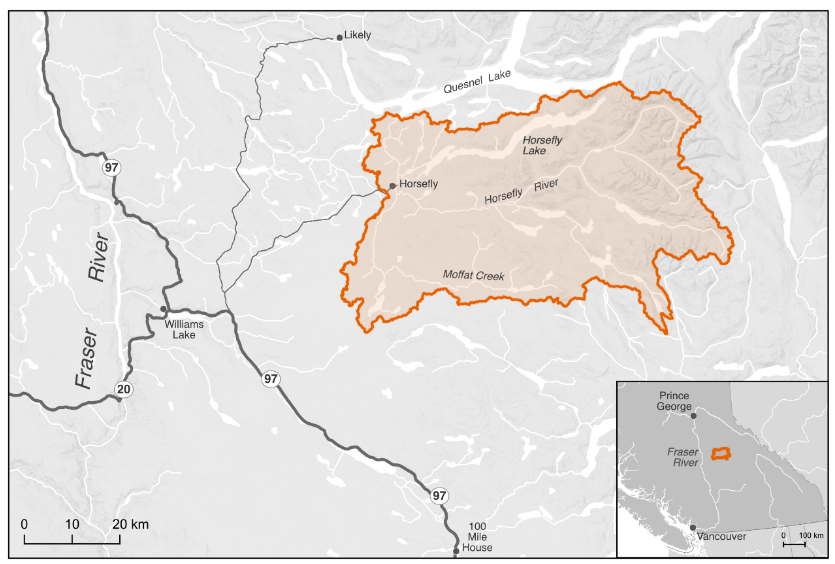
\includegraphics{images/figure1.png}

}

\caption{\label{fig-geoscope}The primary geographic scope --- the
Horsefly River watershed --- located in the Fraser River system.}

\end{figure}

The primary geographic scope of this WCRP is the Horsefly River
watershed, located in the upper Fraser River drainage basin in central
British Columbia (Figure~\ref{fig-geoscope}). The scope constitutes the
Horsefly River ``watershed group'' as defined by the
\href{https://catalogue.data.gov.bc.ca/dataset/freshwater-atlas-watershed-groups}{British
Columbia Freshwater Atlas} (FWA). A consistent spatial framework was
necessary to undertake a watershed selection process at the provincial
scale to identify target watersheds to improve connectivity for salmon.
The Horsefly River watershed was identified by the BC Fish Passage
Restoration Initiative as one of four target watersheds for WCRP
development Mazany-Wright, Norris, et al. (2021b). The Horsefly River
watershed has a drainage area of 276,603 ha, spanning from the Quesnel
Highlands in the southeast to the confluence with Quesnel Lake in the
northwest. Culturally and economically important populations of Chinook
Salmon, Coho Salmon, and Sockeye Salmon are all found in the watershed,
which historically supported Indigenous sustenance and trading economies
(Table~\ref{tbl-targspec}, W. L. F. Nation. (2021), X. F. Nation.
(2021)).

\hypertarget{tbl-targspec}{}
\global\setlength{\Oldarrayrulewidth}{\arrayrulewidth}

\global\setlength{\Oldtabcolsep}{\tabcolsep}

\setlength{\tabcolsep}{0pt}

\renewcommand*{\arraystretch}{1.5}



\providecommand{\ascline}[3]{\noalign{\global\arrayrulewidth #1}\arrayrulecolor[HTML]{#2}\cline{#3}}

\begin{longtable}[c]{|p{1.36in}|p{1.43in}|p{2.15in}}

\caption{\label{tbl-targspec}Target fish species in the Horsefly River watershed. The Secwepemctsín
and Western common and scientific species names are provided. } \\ 


\hhline{>{\arrayrulecolor[HTML]{666666}\global\arrayrulewidth=1.5pt}->{\arrayrulecolor[HTML]{666666}\global\arrayrulewidth=1.5pt}->{\arrayrulecolor[HTML]{666666}\global\arrayrulewidth=1.5pt}-}

\multicolumn{1}{>{\cellcolor[HTML]{008270}\raggedright}m{\dimexpr 1.36in+0\tabcolsep}}{\textcolor[HTML]{FFFFFF}{\fontsize{11}{11}\selectfont{Secwepemctsín}}} & \multicolumn{1}{>{\cellcolor[HTML]{008270}\raggedright}m{\dimexpr 1.43in+0\tabcolsep}}{\textcolor[HTML]{FFFFFF}{\fontsize{11}{11}\selectfont{Common\ Name}}} & \multicolumn{1}{>{\cellcolor[HTML]{008270}\raggedright}m{\dimexpr 2.15in+0\tabcolsep}}{\textcolor[HTML]{FFFFFF}{\fontsize{11}{11}\selectfont{Scientific\ Name}}} \\

\noalign{\global\arrayrulewidth 0pt}\arrayrulecolor[HTML]{000000}

\hhline{>{\arrayrulecolor[HTML]{666666}\global\arrayrulewidth=1.5pt}->{\arrayrulecolor[HTML]{666666}\global\arrayrulewidth=1.5pt}->{\arrayrulecolor[HTML]{666666}\global\arrayrulewidth=1.5pt}-}\endhead



\multicolumn{1}{>{\raggedright}m{\dimexpr 1.36in+0\tabcolsep}}{\textcolor[HTML]{000000}{\fontsize{11}{11}\selectfont{Kekèsu}}} & \multicolumn{1}{>{\raggedright}m{\dimexpr 1.43in+0\tabcolsep}}{\textcolor[HTML]{000000}{\fontsize{11}{11}\selectfont{Chinook\ Salmon}}} & \multicolumn{1}{>{\raggedright}m{\dimexpr 2.15in+0\tabcolsep}}{\textcolor[HTML]{000000}{\fontsize{11}{11}\selectfont{Oncorhynchus\ tshawytscha}}} \\

\noalign{\global\arrayrulewidth 0pt}\arrayrulecolor[HTML]{000000}





\multicolumn{1}{>{\raggedright}m{\dimexpr 1.36in+0\tabcolsep}}{\textcolor[HTML]{000000}{\fontsize{11}{11}\selectfont{Sxeyqs}}} & \multicolumn{1}{>{\raggedright}m{\dimexpr 1.43in+0\tabcolsep}}{\textcolor[HTML]{000000}{\fontsize{11}{11}\selectfont{Coho\ Salmon}}} & \multicolumn{1}{>{\raggedright}m{\dimexpr 2.15in+0\tabcolsep}}{\textcolor[HTML]{000000}{\fontsize{11}{11}\selectfont{Oncorhynchus\ kisutch}}} \\

\noalign{\global\arrayrulewidth 0pt}\arrayrulecolor[HTML]{000000}





\multicolumn{1}{>{\raggedright}m{\dimexpr 1.36in+0\tabcolsep}}{\textcolor[HTML]{000000}{\fontsize{11}{11}\selectfont{Sqlelten7ùwi}}} & \multicolumn{1}{>{\raggedright}m{\dimexpr 1.43in+0\tabcolsep}}{\textcolor[HTML]{000000}{\fontsize{11}{11}\selectfont{Sockeye\ Salmon}}} & \multicolumn{1}{>{\raggedright}m{\dimexpr 2.15in+0\tabcolsep}}{\textcolor[HTML]{000000}{\fontsize{11}{11}\selectfont{Oncorhynchus\ nerka}}} \\

\noalign{\global\arrayrulewidth 0pt}\arrayrulecolor[HTML]{000000}

\hhline{>{\arrayrulecolor[HTML]{666666}\global\arrayrulewidth=1.5pt}->{\arrayrulecolor[HTML]{666666}\global\arrayrulewidth=1.5pt}->{\arrayrulecolor[HTML]{666666}\global\arrayrulewidth=1.5pt}-}



\end{longtable}



\arrayrulecolor[HTML]{000000}

\global\setlength{\arrayrulewidth}{\Oldarrayrulewidth}

\global\setlength{\tabcolsep}{\Oldtabcolsep}

\renewcommand*{\arraystretch}{1}

The Horsefly River watershed comprises parts of Secwepemcúl'ecw, the
traditional territory of the Northern Secwepemc te Qelmucw (NStQ),
represented by the Northern Shuswap Tribal Council and four member
communities or autonomous nations:

\begin{itemize}
\item
  Xatśūll Cmetem' (Soda Creek First Nations)
\item
  Stswēceḿc Xgāt'tem (Canoe Creek/Dog Creek First Nations)
\item
  T'ēxelc (Williams Lake First Nation)
\item
  Tsq'ēsceń (Canim Lake First Nation)
\end{itemize}

The geographic scope of this WCRP was further refined by identifying
``potentially accessible'' stream segments, which are defined as streams
that target species should be able to access in the absence of
anthropogenic barriers (Figure~\ref{fig-strseg}). Potentially accessible
stream segments were spatially delineated using fish species observation
and distribution data, as well as data on ``exclusionary points''. These
include waterfalls greater than 5 m in height, gradient barriers based
on species-specific swimming abilities, and watershed exclusion areas,
which are portions of the watershed where barrier remediation efforts
should not occur. These maps were explored by the planning team to
incorporate additional local knowledge, ensure accuracy, and finalize
the constraints on potentially accessible stream segments. The planning
team identified certain tributaries to the mainstem Horsefly River as
``watershed exclusion areas'', which were excluded from further
consideration under this plan, due to intermittent or insufficient flows
to support restoring connectivity for the target species. The geographic
scope was further refined based on several confirmed impassable
waterfalls and modelled gradient barriers. Specifically, there are two
impassable waterfalls that severely limit potentially accessible
habitat: one on the mainstem Horsefly River approximately 4 km upstream
of the confluence with McKinley Creek, and the second on Moffat Creek
approximately 5 km upstream from where it flows into the Horsefly River.
All stream segments not identified as potentially accessible were
removed from the scope for further consideration. The ``constrained
geographic scope'' formed the foundation for all subsequent analyses and
planning steps, including mapping and modelling useable habitat types,
quantifying the current connectivity status, goal setting, and action
planning Mazany-Wright, Norris, et al. (2021a).

\begin{figure}

{\centering 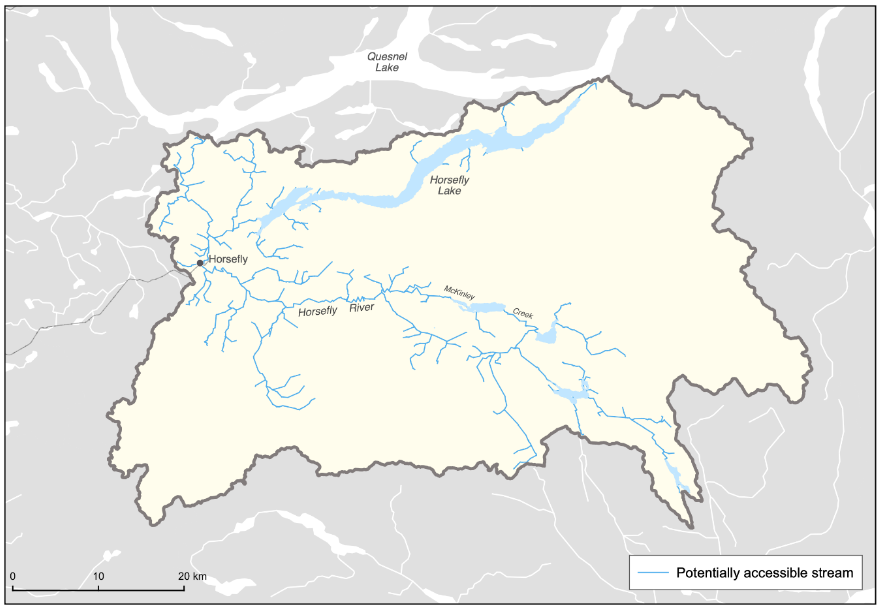
\includegraphics{images/figure2.png}

}

\caption{\label{fig-strseg}Potentially accessible stream segments within
the Horsefly River watershed. These do not represent useable habitat
types, but rather identifies the stream segments within which habitat
modelling and barrier mapping and prioritization was undertaken.}

\end{figure}

\hypertarget{target-species}{%
\section*{Target species}\label{target-species}}
\addcontentsline{toc}{section}{Target species}

\markright{Target species}

Target species represent the ecologically and culturally important
species for which habitat connectivity is being conserved and/or
restored in the watershed. In the Horsefly River watershed, the planning
team selected Anadromous Salmon as the target species group, which
comprises Chinook Salmon, Coho Salmon, and Sockeye Salmon. The selection
of these target species was driven primarily by the targets species of
the primary fund supporting this planning work.

\hypertarget{anadromous-salmonids}{%
\subsection*{Anadromous Salmonids}\label{anadromous-salmonids}}
\addcontentsline{toc}{subsection}{Anadromous Salmonids}

Anadromous salmon are cultural and ecological keystone species that
contribute to productive ecosystems by contributing marine-derived
nutrients to the watershed and forming an important food source for
other species. Salmon species are sacred to the NStQ, having sustained
life, trading economies, and culture since time immemorial (W. L. F.
Nation. (2021), X. F. Nation. (2021), N. Singi pers. comm.). The
stewardship of the resources and fisheries in their traditional
territories are imbued in the spirit of the NStQ through a symbiotic
relationship based on respect -- the NStQ never take more salmon than is
needed and there is no waste. The entirety of the salmon is used -
smoked and dried to sustain the NStQ through the winter months, the roe
harvested for consumption, salmon oil rendered to be stored and traded,
and the skin used to store the oil (Wilson, Twohig, and Dahlstrom
(1998), X. F. Nation. (2021), N. Singi pers. comm.). The salmon runs
begin to return to the Horsefly River watershed in early August, and the
NStQ traditionally celebrate and feast at this time. The harvest of the
salmon strengthens the cultural connection to the land and the waters,
providing an important food source for communities and the opportunity
to pass knowledge and ceremony to future generations through fishing and
fish processing (W. L. F. Nation. (2021)`, X. F. Nation. (2021)).

Anadromous salmon populations in the Horsefly River watershed have
declined significantly in the past few decades, with the populations of
all three focal species being listed as Threatened or Endangered by the
Committee On the Status of Endangered Wildlife In Canada (COSEWIC). This
has been exacerbated by the Big Bar landslide on the Fraser River in
2019, leading the four NStQ communities to voluntarily close the salmon
fishery from 2019-2022. The stewardship of their waters continues
through the work of the NStQ member communities and the Northern Shuswap
Tribal Council. See Appendix A for maps of modelled anadromous salmon
habitat in the Horsefly River Watershed.

\hypertarget{chinook-salmon-kekuxe8su-oncorhynchus-tshawytscha}{%
\subsection*{Chinook Salmon \textbar{} Kekèsu \textbar{} Oncorhynchus
tshawytscha}\label{chinook-salmon-kekuxe8su-oncorhynchus-tshawytscha}}
\addcontentsline{toc}{subsection}{Chinook Salmon \textbar{} Kekèsu
\textbar{} Oncorhynchus tshawytscha}

\hypertarget{tbl-chinook}{}
\global\setlength{\Oldarrayrulewidth}{\arrayrulewidth}

\global\setlength{\Oldtabcolsep}{\tabcolsep}

\setlength{\tabcolsep}{0pt}

\renewcommand*{\arraystretch}{1.5}



\providecommand{\ascline}[3]{\noalign{\global\arrayrulewidth #1}\arrayrulecolor[HTML]{#2}\cline{#3}}

\begin{longtable}[c]{|p{2.76in}|p{1.61in}|p{1.24in}|p{3.55in}|p{3.61in}}

\caption{\label{tbl-chinook}Chinook Salmon population assessments in the Horsefly River watershed.
Conservation Unit assessments were undertaken by the
\href{https://www.salmonexplorer.ca/\#!/fraser/chinook/middle-fraser-river-spring-5-2}{Pacific
Salmon Foundation}
(\href{https://salmonwatersheds.ca/libraryfiles/lib_459.pdf}{2020}).
Designated Unit assessments were undertaken by
\href{https://www.canada.ca/en/environment-climate-change/services/species-risk-public-registry/cosewic-assessments-status-reports/chinook-salmon-2018.html}{COSEWIC}
(2018). } \\ 


\hhline{>{\arrayrulecolor[HTML]{666666}\global\arrayrulewidth=1.5pt}->{\arrayrulecolor[HTML]{666666}\global\arrayrulewidth=1.5pt}->{\arrayrulecolor[HTML]{666666}\global\arrayrulewidth=1.5pt}->{\arrayrulecolor[HTML]{666666}\global\arrayrulewidth=1.5pt}->{\arrayrulecolor[HTML]{666666}\global\arrayrulewidth=1.5pt}-}

\multicolumn{1}{>{\cellcolor[HTML]{008270}\raggedright}m{\dimexpr 2.76in+0\tabcolsep}}{\textcolor[HTML]{FFFFFF}{\fontsize{11}{11}\selectfont{Conservation\ Unit}}} & \multicolumn{1}{>{\cellcolor[HTML]{008270}\raggedright}m{\dimexpr 1.61in+0\tabcolsep}}{\textcolor[HTML]{FFFFFF}{\fontsize{11}{11}\selectfont{Biological\ Status}}} & \multicolumn{1}{>{\cellcolor[HTML]{008270}\raggedright}m{\dimexpr 1.24in+0\tabcolsep}}{\textcolor[HTML]{FFFFFF}{\fontsize{11}{11}\selectfont{Run\ timing}}} & \multicolumn{1}{>{\cellcolor[HTML]{008270}\raggedright}m{\dimexpr 3.55in+0\tabcolsep}}{\textcolor[HTML]{FFFFFF}{\fontsize{11}{11}\selectfont{Trend\ in\ spawner\ abundance\ (all\ available\ data)}}} & \multicolumn{1}{>{\cellcolor[HTML]{008270}\raggedright}m{\dimexpr 3.61in+0\tabcolsep}}{\textcolor[HTML]{FFFFFF}{\fontsize{11}{11}\selectfont{Trend\ in\ spawner\ abundance\ (last\ 3\ generations)}}} \\

\noalign{\global\arrayrulewidth 0pt}\arrayrulecolor[HTML]{000000}

\hhline{>{\arrayrulecolor[HTML]{666666}\global\arrayrulewidth=1.5pt}->{\arrayrulecolor[HTML]{666666}\global\arrayrulewidth=1.5pt}->{\arrayrulecolor[HTML]{666666}\global\arrayrulewidth=1.5pt}->{\arrayrulecolor[HTML]{666666}\global\arrayrulewidth=1.5pt}->{\arrayrulecolor[HTML]{666666}\global\arrayrulewidth=1.5pt}-}\endhead



\multicolumn{1}{>{\raggedright}m{\dimexpr 2.76in+0\tabcolsep}}{\textcolor[HTML]{000000}{\fontsize{11}{11}\selectfont{Middle\ Fraser\ River\ (Spring\ 5-2,\ 1.3)}}} & \multicolumn{1}{>{\raggedright}m{\dimexpr 1.61in+0\tabcolsep}}{\textcolor[HTML]{000000}{\fontsize{11}{11}\selectfont{Data\ Deficient/Poor}}} & \multicolumn{1}{>{\raggedright}m{\dimexpr 1.24in+0\tabcolsep}}{\textcolor[HTML]{000000}{\fontsize{11}{11}\selectfont{Data\ Deficient}}} & \multicolumn{1}{>{\raggedright}m{\dimexpr 3.55in+0\tabcolsep}}{\textcolor[HTML]{000000}{\fontsize{11}{11}\selectfont{Data\ Deficient}}} & \multicolumn{1}{>{\raggedright}m{\dimexpr 3.61in+0\tabcolsep}}{\textcolor[HTML]{000000}{\fontsize{11}{11}\selectfont{Data\ Deficient}}} \\

\noalign{\global\arrayrulewidth 0pt}\arrayrulecolor[HTML]{000000}

\hhline{>{\arrayrulecolor[HTML]{666666}\global\arrayrulewidth=1.5pt}->{\arrayrulecolor[HTML]{666666}\global\arrayrulewidth=1.5pt}->{\arrayrulecolor[HTML]{666666}\global\arrayrulewidth=1.5pt}->{\arrayrulecolor[HTML]{666666}\global\arrayrulewidth=1.5pt}->{\arrayrulecolor[HTML]{666666}\global\arrayrulewidth=1.5pt}-}



\end{longtable}



\arrayrulecolor[HTML]{000000}

\global\setlength{\arrayrulewidth}{\Oldarrayrulewidth}

\global\setlength{\tabcolsep}{\Oldtabcolsep}

\renewcommand*{\arraystretch}{1}

\global\setlength{\Oldarrayrulewidth}{\arrayrulewidth}

\global\setlength{\Oldtabcolsep}{\tabcolsep}

\setlength{\tabcolsep}{0pt}

\renewcommand*{\arraystretch}{1.5}



\providecommand{\ascline}[3]{\noalign{\global\arrayrulewidth #1}\arrayrulecolor[HTML]{#2}\cline{#3}}

\begin{longtable*}[c]{|p{4.13in}|p{1.07in}|p{0.91in}|p{3.23in}|p{2.51in}|p{1.50in}}



\hhline{>{\arrayrulecolor[HTML]{666666}\global\arrayrulewidth=1.5pt}->{\arrayrulecolor[HTML]{666666}\global\arrayrulewidth=1.5pt}->{\arrayrulecolor[HTML]{666666}\global\arrayrulewidth=1.5pt}->{\arrayrulecolor[HTML]{666666}\global\arrayrulewidth=1.5pt}->{\arrayrulecolor[HTML]{666666}\global\arrayrulewidth=1.5pt}->{\arrayrulecolor[HTML]{666666}\global\arrayrulewidth=1.5pt}-}

\multicolumn{1}{>{\cellcolor[HTML]{008270}\raggedright}m{\dimexpr 4.13in+0\tabcolsep}}{\textcolor[HTML]{FFFFFF}{\fontsize{11}{11}\selectfont{COSEWIC\ Designated\ Unit}}} & \multicolumn{1}{>{\cellcolor[HTML]{008270}\raggedright}m{\dimexpr 1.07in+0\tabcolsep}}{\textcolor[HTML]{FFFFFF}{\fontsize{11}{11}\selectfont{Status}}} & \multicolumn{1}{>{\cellcolor[HTML]{008270}\raggedright}m{\dimexpr 0.91in+0\tabcolsep}}{\textcolor[HTML]{FFFFFF}{\fontsize{11}{11}\selectfont{Trend}}} & \multicolumn{1}{>{\cellcolor[HTML]{008270}\raggedright}m{\dimexpr 3.23in+0\tabcolsep}}{\textcolor[HTML]{FFFFFF}{\fontsize{11}{11}\selectfont{Median\ percent\ change\ (last\ 3\ generations)}}} & \multicolumn{1}{>{\cellcolor[HTML]{008270}\raggedright}m{\dimexpr 2.51in+0\tabcolsep}}{\textcolor[HTML]{FFFFFF}{\fontsize{11}{11}\selectfont{Median\ percent\ change\ (historic)}}} & \multicolumn{1}{>{\cellcolor[HTML]{008270}\raggedright}m{\dimexpr 1.5in+0\tabcolsep}}{\textcolor[HTML]{FFFFFF}{\fontsize{11}{11}\selectfont{Generation\ length}}} \\

\noalign{\global\arrayrulewidth 0pt}\arrayrulecolor[HTML]{000000}

\hhline{>{\arrayrulecolor[HTML]{666666}\global\arrayrulewidth=1.5pt}->{\arrayrulecolor[HTML]{666666}\global\arrayrulewidth=1.5pt}->{\arrayrulecolor[HTML]{666666}\global\arrayrulewidth=1.5pt}->{\arrayrulecolor[HTML]{666666}\global\arrayrulewidth=1.5pt}->{\arrayrulecolor[HTML]{666666}\global\arrayrulewidth=1.5pt}->{\arrayrulecolor[HTML]{666666}\global\arrayrulewidth=1.5pt}-}\endhead



\multicolumn{1}{>{\raggedright}m{\dimexpr 4.13in+0\tabcolsep}}{\textcolor[HTML]{000000}{\fontsize{11}{11}\selectfont{9-\ Middle\ Fraser,\ Stream,\ Spring\ (MFR+GStr)\ population}}} & \multicolumn{1}{>{\raggedright}m{\dimexpr 1.07in+0\tabcolsep}}{\textcolor[HTML]{000000}{\fontsize{11}{11}\selectfont{Threatened}}} & \multicolumn{1}{>{\raggedright}m{\dimexpr 0.91in+0\tabcolsep}}{\textcolor[HTML]{000000}{\fontsize{11}{11}\selectfont{Declining}}} & \multicolumn{1}{>{\raggedright}m{\dimexpr 3.23in+0\tabcolsep}}{\textcolor[HTML]{000000}{\fontsize{11}{11}\selectfont{-28\%}}} & \multicolumn{1}{>{\raggedright}m{\dimexpr 2.51in+0\tabcolsep}}{\textcolor[HTML]{000000}{\fontsize{11}{11}\selectfont{-49\%}}} & \multicolumn{1}{>{\raggedright}m{\dimexpr 1.5in+0\tabcolsep}}{\textcolor[HTML]{000000}{\fontsize{11}{11}\selectfont{4.5\ years}}} \\

\noalign{\global\arrayrulewidth 0pt}\arrayrulecolor[HTML]{000000}

\hhline{>{\arrayrulecolor[HTML]{666666}\global\arrayrulewidth=1.5pt}->{\arrayrulecolor[HTML]{666666}\global\arrayrulewidth=1.5pt}->{\arrayrulecolor[HTML]{666666}\global\arrayrulewidth=1.5pt}->{\arrayrulecolor[HTML]{666666}\global\arrayrulewidth=1.5pt}->{\arrayrulecolor[HTML]{666666}\global\arrayrulewidth=1.5pt}->{\arrayrulecolor[HTML]{666666}\global\arrayrulewidth=1.5pt}-}



\end{longtable*}



\arrayrulecolor[HTML]{000000}

\global\setlength{\arrayrulewidth}{\Oldarrayrulewidth}

\global\setlength{\tabcolsep}{\Oldtabcolsep}

\renewcommand*{\arraystretch}{1}

Chinook Salmon are the first to return each year, usually in early
August DFO (1991), and have the most limited distribution within the
watershed. Known spawning occurs in parts of the Horsefly River mainstem
above the confluence with the Little Horsefly River and throughout
McKinley Creek as far as Elbow Lake (DFO (1991), S. Hocquard, pers.
comm.). Important rearing systems include Patenaude Creek, Kroener
Creek, Black Creek, Woodjam Creek, Deerhorn Creek, and Wilmot Creek (S.
Hocquard, pers. comm.).

\hypertarget{coho-salmon-sxeyqs-oncorhynchus-kisutch}{%
\subsection*{Coho Salmon \textbar{} Sxeyqs \textbar{} Oncorhynchus
kisutch}\label{coho-salmon-sxeyqs-oncorhynchus-kisutch}}
\addcontentsline{toc}{subsection}{Coho Salmon \textbar{} Sxeyqs
\textbar{} Oncorhynchus kisutch}

\hypertarget{tbl-coho}{}
\global\setlength{\Oldarrayrulewidth}{\arrayrulewidth}

\global\setlength{\Oldtabcolsep}{\tabcolsep}

\setlength{\tabcolsep}{0pt}

\renewcommand*{\arraystretch}{1.5}



\providecommand{\ascline}[3]{\noalign{\global\arrayrulewidth #1}\arrayrulecolor[HTML]{#2}\cline{#3}}

\begin{longtable}[c]{|p{1.50in}|p{1.55in}|p{1.24in}|p{3.55in}|p{3.61in}}

\caption{\label{tbl-coho}Coho Salmon population assessments in the Horsefly River watershed.
Conservation Unit assessments were undertaken by the
\href{https://www.salmonexplorer.ca/\#!/fraser/chinook/middle-fraser-river-spring-5-2}{Pacific
Salmon Foundation}
(\href{https://salmonwatersheds.ca/libraryfiles/lib_459.pdf}{2020}).
Designated Unit assessments were undertaken by
\href{https://www.canada.ca/en/environment-climate-change/services/species-risk-public-registry/cosewic-assessments-status-reports/chinook-salmon-2018.html}{COSEWIC}
(2018). } \\ 


\hhline{>{\arrayrulecolor[HTML]{666666}\global\arrayrulewidth=1.5pt}->{\arrayrulecolor[HTML]{666666}\global\arrayrulewidth=1.5pt}->{\arrayrulecolor[HTML]{666666}\global\arrayrulewidth=1.5pt}->{\arrayrulecolor[HTML]{666666}\global\arrayrulewidth=1.5pt}->{\arrayrulecolor[HTML]{666666}\global\arrayrulewidth=1.5pt}-}

\multicolumn{1}{>{\cellcolor[HTML]{008270}\raggedright}m{\dimexpr 1.5in+0\tabcolsep}}{\textcolor[HTML]{FFFFFF}{\fontsize{11}{11}\selectfont{Conservation\ Unit}}} & \multicolumn{1}{>{\cellcolor[HTML]{008270}\raggedright}m{\dimexpr 1.55in+0\tabcolsep}}{\textcolor[HTML]{FFFFFF}{\fontsize{11}{11}\selectfont{Biological\ Status}}} & \multicolumn{1}{>{\cellcolor[HTML]{008270}\raggedright}m{\dimexpr 1.24in+0\tabcolsep}}{\textcolor[HTML]{FFFFFF}{\fontsize{11}{11}\selectfont{Run\ timing}}} & \multicolumn{1}{>{\cellcolor[HTML]{008270}\raggedright}m{\dimexpr 3.55in+0\tabcolsep}}{\textcolor[HTML]{FFFFFF}{\fontsize{11}{11}\selectfont{Trend\ in\ spawner\ abundance\ (all\ available\ data)}}} & \multicolumn{1}{>{\cellcolor[HTML]{008270}\raggedright}m{\dimexpr 3.61in+0\tabcolsep}}{\textcolor[HTML]{FFFFFF}{\fontsize{11}{11}\selectfont{Trend\ in\ spawner\ abundance\ (last\ 3\ generations)}}} \\

\noalign{\global\arrayrulewidth 0pt}\arrayrulecolor[HTML]{000000}

\hhline{>{\arrayrulecolor[HTML]{666666}\global\arrayrulewidth=1.5pt}->{\arrayrulecolor[HTML]{666666}\global\arrayrulewidth=1.5pt}->{\arrayrulecolor[HTML]{666666}\global\arrayrulewidth=1.5pt}->{\arrayrulecolor[HTML]{666666}\global\arrayrulewidth=1.5pt}->{\arrayrulecolor[HTML]{666666}\global\arrayrulewidth=1.5pt}-}\endhead



\multicolumn{1}{>{\raggedright}m{\dimexpr 1.5in+0\tabcolsep}}{\textcolor[HTML]{000000}{\fontsize{11}{11}\selectfont{Interior\ Fraser}}} & \multicolumn{1}{>{\raggedright}m{\dimexpr 1.55in+0\tabcolsep}}{\textcolor[HTML]{000000}{\fontsize{11}{11}\selectfont{Data\ Deficient/Fair}}} & \multicolumn{1}{>{\raggedright}m{\dimexpr 1.24in+0\tabcolsep}}{\textcolor[HTML]{000000}{\fontsize{11}{11}\selectfont{Data\ Deficient}}} & \multicolumn{1}{>{\raggedright}m{\dimexpr 3.55in+0\tabcolsep}}{\textcolor[HTML]{000000}{\fontsize{11}{11}\selectfont{Data\ Deficient}}} & \multicolumn{1}{>{\raggedright}m{\dimexpr 3.61in+0\tabcolsep}}{\textcolor[HTML]{000000}{\fontsize{11}{11}\selectfont{Data\ Deficient}}} \\

\noalign{\global\arrayrulewidth 0pt}\arrayrulecolor[HTML]{000000}

\hhline{>{\arrayrulecolor[HTML]{666666}\global\arrayrulewidth=1.5pt}->{\arrayrulecolor[HTML]{666666}\global\arrayrulewidth=1.5pt}->{\arrayrulecolor[HTML]{666666}\global\arrayrulewidth=1.5pt}->{\arrayrulecolor[HTML]{666666}\global\arrayrulewidth=1.5pt}->{\arrayrulecolor[HTML]{666666}\global\arrayrulewidth=1.5pt}-}



\end{longtable}



\arrayrulecolor[HTML]{000000}

\global\setlength{\arrayrulewidth}{\Oldarrayrulewidth}

\global\setlength{\tabcolsep}{\Oldtabcolsep}

\renewcommand*{\arraystretch}{1}

\global\setlength{\Oldarrayrulewidth}{\arrayrulewidth}

\global\setlength{\Oldtabcolsep}{\tabcolsep}

\setlength{\tabcolsep}{0pt}

\renewcommand*{\arraystretch}{1.5}



\providecommand{\ascline}[3]{\noalign{\global\arrayrulewidth #1}\arrayrulecolor[HTML]{#2}\cline{#3}}

\begin{longtable*}[c]{|p{3.35in}|p{1.07in}|p{0.91in}|p{3.23in}|p{8.25in}|p{1.50in}}



\hhline{>{\arrayrulecolor[HTML]{666666}\global\arrayrulewidth=1.5pt}->{\arrayrulecolor[HTML]{666666}\global\arrayrulewidth=1.5pt}->{\arrayrulecolor[HTML]{666666}\global\arrayrulewidth=1.5pt}->{\arrayrulecolor[HTML]{666666}\global\arrayrulewidth=1.5pt}->{\arrayrulecolor[HTML]{666666}\global\arrayrulewidth=1.5pt}->{\arrayrulecolor[HTML]{666666}\global\arrayrulewidth=1.5pt}-}

\multicolumn{1}{>{\cellcolor[HTML]{008270}\raggedright}m{\dimexpr 3.35in+0\tabcolsep}}{\textcolor[HTML]{FFFFFF}{\fontsize{11}{11}\selectfont{COSEWIC\ Designated\ Unit}}} & \multicolumn{1}{>{\cellcolor[HTML]{008270}\raggedright}m{\dimexpr 1.07in+0\tabcolsep}}{\textcolor[HTML]{FFFFFF}{\fontsize{11}{11}\selectfont{Status}}} & \multicolumn{1}{>{\cellcolor[HTML]{008270}\raggedright}m{\dimexpr 0.91in+0\tabcolsep}}{\textcolor[HTML]{FFFFFF}{\fontsize{11}{11}\selectfont{Trend}}} & \multicolumn{1}{>{\cellcolor[HTML]{008270}\raggedright}m{\dimexpr 3.23in+0\tabcolsep}}{\textcolor[HTML]{FFFFFF}{\fontsize{11}{11}\selectfont{Median\ percent\ change\ (last\ 3\ generations)}}} & \multicolumn{1}{>{\cellcolor[HTML]{008270}\raggedright}m{\dimexpr 8.25in+0\tabcolsep}}{\textcolor[HTML]{FFFFFF}{\fontsize{11}{11}\selectfont{Median\ percent\ change\ (historic)}}} & \multicolumn{1}{>{\cellcolor[HTML]{008270}\raggedright}m{\dimexpr 1.5in+0\tabcolsep}}{\textcolor[HTML]{FFFFFF}{\fontsize{11}{11}\selectfont{Generation\ length}}} \\

\noalign{\global\arrayrulewidth 0pt}\arrayrulecolor[HTML]{000000}

\hhline{>{\arrayrulecolor[HTML]{666666}\global\arrayrulewidth=1.5pt}->{\arrayrulecolor[HTML]{666666}\global\arrayrulewidth=1.5pt}->{\arrayrulecolor[HTML]{666666}\global\arrayrulewidth=1.5pt}->{\arrayrulecolor[HTML]{666666}\global\arrayrulewidth=1.5pt}->{\arrayrulecolor[HTML]{666666}\global\arrayrulewidth=1.5pt}->{\arrayrulecolor[HTML]{666666}\global\arrayrulewidth=1.5pt}-}\endhead



\multicolumn{1}{>{\raggedright}m{\dimexpr 3.35in+0\tabcolsep}}{\textcolor[HTML]{000000}{\fontsize{11}{11}\selectfont{Interior\ Fraser\ –\ Mid/Upper\ Fraser\ population}}} & \multicolumn{1}{>{\raggedright}m{\dimexpr 1.07in+0\tabcolsep}}{\textcolor[HTML]{000000}{\fontsize{11}{11}\selectfont{Threatened}}} & \multicolumn{1}{>{\raggedright}m{\dimexpr 0.91in+0\tabcolsep}}{\textcolor[HTML]{000000}{\fontsize{11}{11}\selectfont{Declining}}} & \multicolumn{1}{>{\raggedright}m{\dimexpr 3.23in+0\tabcolsep}}{\textcolor[HTML]{000000}{\fontsize{11}{11}\selectfont{Not\ estimated}}} & \multicolumn{1}{>{\raggedright}m{\dimexpr 8.25in+0\tabcolsep}}{\textcolor[HTML]{000000}{\fontsize{11}{11}\selectfont{+119\%\ estimated\ based\ on\ last\ 10\ years\ of\ escapement\ data-21\%\ estimated\ based\ on\ entire\ escapement\ time\ series}}} & \multicolumn{1}{>{\raggedright}m{\dimexpr 1.5in+0\tabcolsep}}{\textcolor[HTML]{000000}{\fontsize{11}{11}\selectfont{3\ years}}} \\

\noalign{\global\arrayrulewidth 0pt}\arrayrulecolor[HTML]{000000}

\hhline{>{\arrayrulecolor[HTML]{666666}\global\arrayrulewidth=1.5pt}->{\arrayrulecolor[HTML]{666666}\global\arrayrulewidth=1.5pt}->{\arrayrulecolor[HTML]{666666}\global\arrayrulewidth=1.5pt}->{\arrayrulecolor[HTML]{666666}\global\arrayrulewidth=1.5pt}->{\arrayrulecolor[HTML]{666666}\global\arrayrulewidth=1.5pt}->{\arrayrulecolor[HTML]{666666}\global\arrayrulewidth=1.5pt}-}



\end{longtable*}



\arrayrulecolor[HTML]{000000}

\global\setlength{\arrayrulewidth}{\Oldarrayrulewidth}

\global\setlength{\tabcolsep}{\Oldtabcolsep}

\renewcommand*{\arraystretch}{1}

Coho Salmon are the most widely distributed of the three focal species
in the watershed, with the ability to migrate into smaller, upper
tributary systems DFO (1991). Spawning occurs in the Little Horsefly
River between Gruhs Lake and Horsefly Lake, McKinley Creek below
McKinley Lake, Woodjam Creek, Patenaude Creek, Tisdall Creek, and Black
Creek. Rearing fry and juveniles have been observed in the Little
Horsefly River, Patenaude Creek, and McKinley Creek up to Bosk Lake (DFO
(1991), S. Hocquard pers. comm.).

\hypertarget{sockeye-salmon-sqlelten7uxf9wi-oncorhynchus-nerka}{%
\subsection*{Sockeye Salmon \textbar{} Sqlelten7ùwi \textbar{}
Oncorhynchus
nerka}\label{sockeye-salmon-sqlelten7uxf9wi-oncorhynchus-nerka}}
\addcontentsline{toc}{subsection}{Sockeye Salmon \textbar{} Sqlelten7ùwi
\textbar{} Oncorhynchus nerka}

\hypertarget{tbl-sockeye}{}
\global\setlength{\Oldarrayrulewidth}{\arrayrulewidth}

\global\setlength{\Oldtabcolsep}{\tabcolsep}

\setlength{\tabcolsep}{0pt}

\renewcommand*{\arraystretch}{1.5}



\providecommand{\ascline}[3]{\noalign{\global\arrayrulewidth #1}\arrayrulecolor[HTML]{#2}\cline{#3}}

\begin{longtable}[c]{|p{2.00in}|p{1.92in}|p{1.36in}|p{3.40in}|p{3.61in}}

\caption{\label{tbl-sockeye}Sockeye Salmon population assessments in the Horsefly River watershed.
Conservation Unit assessments were undertaken by the
\href{https://www.salmonexplorer.ca/\#!/fraser/chinook/middle-fraser-river-spring-5-2}{Pacific
Salmon Foundation}
(\href{https://salmonwatersheds.ca/libraryfiles/lib_459.pdf}{2020}).
Designated Unit assessments were undertaken by
\href{https://www.canada.ca/en/environment-climate-change/services/species-risk-public-registry/cosewic-assessments-status-reports/chinook-salmon-2018.html}{COSEWIC}
(2018). } \\ 


\hhline{>{\arrayrulecolor[HTML]{666666}\global\arrayrulewidth=1.5pt}->{\arrayrulecolor[HTML]{666666}\global\arrayrulewidth=1.5pt}->{\arrayrulecolor[HTML]{666666}\global\arrayrulewidth=1.5pt}->{\arrayrulecolor[HTML]{666666}\global\arrayrulewidth=1.5pt}->{\arrayrulecolor[HTML]{666666}\global\arrayrulewidth=1.5pt}-}

\multicolumn{1}{>{\cellcolor[HTML]{008270}\raggedright}m{\dimexpr 2in+0\tabcolsep}}{\textcolor[HTML]{FFFFFF}{\fontsize{11}{11}\selectfont{Conservation\ Unit}}} & \multicolumn{1}{>{\cellcolor[HTML]{008270}\raggedright}m{\dimexpr 1.92in+0\tabcolsep}}{\textcolor[HTML]{FFFFFF}{\fontsize{11}{11}\selectfont{Biological\ Status}}} & \multicolumn{1}{>{\cellcolor[HTML]{008270}\raggedright}m{\dimexpr 1.36in+0\tabcolsep}}{\textcolor[HTML]{FFFFFF}{\fontsize{11}{11}\selectfont{Run\ timing}}} & \multicolumn{1}{>{\cellcolor[HTML]{008270}\raggedright}m{\dimexpr 3.4in+0\tabcolsep}}{\textcolor[HTML]{FFFFFF}{\fontsize{11}{11}\selectfont{Trend\ in\ spawner\ abundance\ (all\ generations)}}} & \multicolumn{1}{>{\cellcolor[HTML]{008270}\raggedright}m{\dimexpr 3.61in+0\tabcolsep}}{\textcolor[HTML]{FFFFFF}{\fontsize{11}{11}\selectfont{Trend\ in\ spawner\ abundance\ (last\ 3\ generations)}}} \\

\noalign{\global\arrayrulewidth 0pt}\arrayrulecolor[HTML]{000000}

\hhline{>{\arrayrulecolor[HTML]{666666}\global\arrayrulewidth=1.5pt}->{\arrayrulecolor[HTML]{666666}\global\arrayrulewidth=1.5pt}->{\arrayrulecolor[HTML]{666666}\global\arrayrulewidth=1.5pt}->{\arrayrulecolor[HTML]{666666}\global\arrayrulewidth=1.5pt}->{\arrayrulecolor[HTML]{666666}\global\arrayrulewidth=1.5pt}-}\endhead



\multicolumn{1}{>{\raggedright}m{\dimexpr 2in+0\tabcolsep}}{\textcolor[HTML]{000000}{\fontsize{11}{11}\selectfont{Quesnel-Summer\ (cyclic)}}} & \multicolumn{1}{>{\raggedright}m{\dimexpr 1.92in+0\tabcolsep}}{\textcolor[HTML]{000000}{\fontsize{11}{11}\selectfont{Data\ Deficient/Fair-Poor}}} & \multicolumn{1}{>{\raggedright}m{\dimexpr 1.36in+0\tabcolsep}}{\textcolor[HTML]{000000}{\fontsize{11}{11}\selectfont{July-September}}} & \multicolumn{1}{>{\raggedright}m{\dimexpr 3.4in+0\tabcolsep}}{\textcolor[HTML]{000000}{\fontsize{11}{11}\selectfont{Data\ Deficient}}} & \multicolumn{1}{>{\raggedright}m{\dimexpr 3.61in+0\tabcolsep}}{\textcolor[HTML]{000000}{\fontsize{11}{11}\selectfont{Data\ Deficient}}} \\

\noalign{\global\arrayrulewidth 0pt}\arrayrulecolor[HTML]{000000}

\hhline{>{\arrayrulecolor[HTML]{666666}\global\arrayrulewidth=1.5pt}->{\arrayrulecolor[HTML]{666666}\global\arrayrulewidth=1.5pt}->{\arrayrulecolor[HTML]{666666}\global\arrayrulewidth=1.5pt}->{\arrayrulecolor[HTML]{666666}\global\arrayrulewidth=1.5pt}->{\arrayrulecolor[HTML]{666666}\global\arrayrulewidth=1.5pt}-}



\end{longtable}



\arrayrulecolor[HTML]{000000}

\global\setlength{\arrayrulewidth}{\Oldarrayrulewidth}

\global\setlength{\tabcolsep}{\Oldtabcolsep}

\renewcommand*{\arraystretch}{1}

\global\setlength{\Oldarrayrulewidth}{\arrayrulewidth}

\global\setlength{\Oldtabcolsep}{\tabcolsep}

\setlength{\tabcolsep}{0pt}

\renewcommand*{\arraystretch}{1.5}



\providecommand{\ascline}[3]{\noalign{\global\arrayrulewidth #1}\arrayrulecolor[HTML]{#2}\cline{#3}}

\begin{longtable*}[c]{|p{2.14in}|p{1.12in}|p{0.91in}|p{3.23in}|p{2.51in}|p{1.50in}}



\hhline{>{\arrayrulecolor[HTML]{666666}\global\arrayrulewidth=1.5pt}->{\arrayrulecolor[HTML]{666666}\global\arrayrulewidth=1.5pt}->{\arrayrulecolor[HTML]{666666}\global\arrayrulewidth=1.5pt}->{\arrayrulecolor[HTML]{666666}\global\arrayrulewidth=1.5pt}->{\arrayrulecolor[HTML]{666666}\global\arrayrulewidth=1.5pt}->{\arrayrulecolor[HTML]{666666}\global\arrayrulewidth=1.5pt}-}

\multicolumn{1}{>{\cellcolor[HTML]{008270}\raggedright}m{\dimexpr 2.14in+0\tabcolsep}}{\textcolor[HTML]{FFFFFF}{\fontsize{11}{11}\selectfont{COSEWIC\ Designated\ Unit}}} & \multicolumn{1}{>{\cellcolor[HTML]{008270}\raggedright}m{\dimexpr 1.12in+0\tabcolsep}}{\textcolor[HTML]{FFFFFF}{\fontsize{11}{11}\selectfont{Status}}} & \multicolumn{1}{>{\cellcolor[HTML]{008270}\raggedright}m{\dimexpr 0.91in+0\tabcolsep}}{\textcolor[HTML]{FFFFFF}{\fontsize{11}{11}\selectfont{Trend}}} & \multicolumn{1}{>{\cellcolor[HTML]{008270}\raggedright}m{\dimexpr 3.23in+0\tabcolsep}}{\textcolor[HTML]{FFFFFF}{\fontsize{11}{11}\selectfont{Median\ percent\ change\ (last\ 3\ generations)}}} & \multicolumn{1}{>{\cellcolor[HTML]{008270}\raggedright}m{\dimexpr 2.51in+0\tabcolsep}}{\textcolor[HTML]{FFFFFF}{\fontsize{11}{11}\selectfont{Median\ percent\ change\ (historic)}}} & \multicolumn{1}{>{\cellcolor[HTML]{008270}\raggedright}m{\dimexpr 1.5in+0\tabcolsep}}{\textcolor[HTML]{FFFFFF}{\fontsize{11}{11}\selectfont{Generation\ length}}} \\

\noalign{\global\arrayrulewidth 0pt}\arrayrulecolor[HTML]{000000}

\hhline{>{\arrayrulecolor[HTML]{666666}\global\arrayrulewidth=1.5pt}->{\arrayrulecolor[HTML]{666666}\global\arrayrulewidth=1.5pt}->{\arrayrulecolor[HTML]{666666}\global\arrayrulewidth=1.5pt}->{\arrayrulecolor[HTML]{666666}\global\arrayrulewidth=1.5pt}->{\arrayrulecolor[HTML]{666666}\global\arrayrulewidth=1.5pt}->{\arrayrulecolor[HTML]{666666}\global\arrayrulewidth=1.5pt}-}\endhead



\multicolumn{1}{>{\raggedright}m{\dimexpr 2.14in+0\tabcolsep}}{\textcolor[HTML]{000000}{\fontsize{11}{11}\selectfont{16\ -Quesnel-S\ population}}} & \multicolumn{1}{>{\raggedright}m{\dimexpr 1.12in+0\tabcolsep}}{\textcolor[HTML]{000000}{\fontsize{11}{11}\selectfont{Endangered}}} & \multicolumn{1}{>{\raggedright}m{\dimexpr 0.91in+0\tabcolsep}}{\textcolor[HTML]{000000}{\fontsize{11}{11}\selectfont{Declining}}} & \multicolumn{1}{>{\raggedright}m{\dimexpr 3.23in+0\tabcolsep}}{\textcolor[HTML]{000000}{\fontsize{11}{11}\selectfont{260,974}}} & \multicolumn{1}{>{\raggedright}m{\dimexpr 2.51in+0\tabcolsep}}{\textcolor[HTML]{000000}{\fontsize{11}{11}\selectfont{-97\%}}} & \multicolumn{1}{>{\raggedright}m{\dimexpr 1.5in+0\tabcolsep}}{\textcolor[HTML]{000000}{\fontsize{11}{11}\selectfont{272\%}}} \\

\noalign{\global\arrayrulewidth 0pt}\arrayrulecolor[HTML]{000000}

\hhline{>{\arrayrulecolor[HTML]{666666}\global\arrayrulewidth=1.5pt}->{\arrayrulecolor[HTML]{666666}\global\arrayrulewidth=1.5pt}->{\arrayrulecolor[HTML]{666666}\global\arrayrulewidth=1.5pt}->{\arrayrulecolor[HTML]{666666}\global\arrayrulewidth=1.5pt}->{\arrayrulecolor[HTML]{666666}\global\arrayrulewidth=1.5pt}->{\arrayrulecolor[HTML]{666666}\global\arrayrulewidth=1.5pt}-}



\end{longtable*}



\arrayrulecolor[HTML]{000000}

\global\setlength{\arrayrulewidth}{\Oldarrayrulewidth}

\global\setlength{\tabcolsep}{\Oldtabcolsep}

\renewcommand*{\arraystretch}{1}

Sockeye Salmon have historically been the most abundant of the three
focal species in the watershed, though the population has seen
significant declines in recent years (DFO (1991), S. Hocquard pers.
comm.). Sockeye Salmon spawning is known to occur throughout the
Horsefly River (up to the impassable falls), in the Little Horsefly
River between Gruhs Lake and Horsefly Lake, Moffat Creek (up to the
impassible falls), and McKinley Creek up to Elbow Lake
(Pacific-Salmon-Foundation (2020), DFO (1991), S. Hocquard pers. comm.).
Additionally, a spawning channel aimed at enhancing the Sockeye Salmon
population was constructed by Fisheries and Oceans Canada in 1989 DFO
(1991). Currently, there are no Sockeye Salmon rearing in the Horsefly
River watershed -- all emergent fry migrate down to Quesnel Lake.

\bookmarksetup{startatroot}

\hypertarget{connectivity-status-assessment-and-action-plan}{%
\chapter*{Connectivity Status Assessment and Action
Plan}\label{connectivity-status-assessment-and-action-plan}}
\addcontentsline{toc}{chapter}{Connectivity Status Assessment and Action
Plan}

\markboth{Connectivity Status Assessment and Action Plan}{Connectivity
Status Assessment and Action Plan}

The planning team devised two Key Ecological Attributes (KEAs) and
associated indicators to assess the current connectivity status of the
watershed -- Accessible Habitat and Accessible Overwintering Habitat
(Table~\ref{tbl-connectivity}). KEAs are the key aspects of anadromous
salmon ecology that are being targeted by this WCRP. The connectivity
status of Anadromous Salmon was used to establish goals to improve
habitat connectivity in the watershed and will be the baseline against
which progress is tracked over time.

The current connectivity status assessment relies on GIS analyses to map
known and modelled barriers to fish passage, identify stream reaches
that have potential spawning and rearing habitat, estimate the
proportion of habitat that is currently accessible to target species,
and prioritize barriers for field assessment that would provide the
greatest gains in connectivity. To support a flexible prioritization
framework to identify priority barriers in the watershed, two
assumptions are made: 1,any modelled (i.e., passability status is
unknown) or partial barriers are treated as complete barriers to passage
and 2, the habitat modelling is binary, it does not assign any habitat
quality values. As such, the current connectivity status will be refined
over time as more data on habitat and barriers are collected. For more
detail on how the connectivity status assessments were conducted, see
Appendix B.

\hypertarget{tbl-connectivity}{}
\begin{longtable}[]{@{}lllllll@{}}
\caption{\label{tbl-connectivity}Connectivity status assessment for (a)
linear habitat (spawning and rearing) and (b) overwintering habitat in
the Horsefly River watershed. The Available Habitat KEA is evaluated by
dividing the length of linear habitat that is currently accessible to
target species by the total length of all linear habitat in the
watershed. The Available Overwintering Habitat KEA is evaluated as the
sum of all areal overwintering habitat that is accessible to target
species.}\label{T_2ba00_}\tabularnewline
\toprule\noalign{}
Target Species & KEA & Indicator & Poor & Fair & Good & Very Good \\
\midrule\noalign{}
\endfirsthead
\toprule\noalign{}
Target Species & KEA & Indicator & Poor & Fair & Good & Very Good \\
\midrule\noalign{}
\endhead
\bottomrule\noalign{}
\endlastfoot
Andromous Salmon & Available Habitat & \% of total linear habitat &
\textless80\% & & 81-90\% & \textgreater90\% \\
& & Current Status: & & & & 91 \\
\end{longtable}

\textbf{Comments:} Indicator rating definitions are based on the
consensus decisions of the planning team, including the decision not to
define Fair. The current status is based on the CWF Barrier
Prioritization Model output, which is current as of March 2022.

\begin{longtable}[]{@{}lllllll@{}}
\caption{}\label{T_00546_}\tabularnewline
\toprule\noalign{}
Target Species & KEA & Indicator & Poor & Fair & Good & Very Good \\
\midrule\noalign{}
\endfirsthead
\toprule\noalign{}
Target Species & KEA & Indicator & Poor & Fair & Good & Very Good \\
\midrule\noalign{}
\endhead
\bottomrule\noalign{}
\endlastfoot
Andromous Salmon & Available Overwintering Habitat & Total Area (m2) of
overwintering habitat accessible & ? & ? & ? & ? \\
& & Current Status: & & & & \\
\end{longtable}

\textbf{Comments:} No baseline data exists on the extent of
overwintering habitat in the watershed. A priority action is included in
the Operational Plan (strategy 2.3) to develop a habitat layer, and this
will be used to inform this connectivity status assessment in the
future.

\hypertarget{barrier-types}{%
\section*{Barrier Types}\label{barrier-types}}
\addcontentsline{toc}{section}{Barrier Types}

\markright{Barrier Types}

The following table highlights which barrier types pose the greatest
threat to anadromous salmon in the watershed. The results of this
assessment were used to inform the subsequent planning steps, as well as
to identify knowledge gaps where there is little spatial data to inform
the assessment for a specific barrier type.

\hypertarget{tbl-barriertype}{}
\begin{longtable}[]{@{}lllll@{}}
\caption{\label{tbl-barriertype}Connectivity status assessment for (a)
linear habitat (spawning and rearing) and (b) overwintering habitat in
the Horsefly River watershed. The Available Habitat KEA is evaluated by
dividing the length of linear habitat that is currently accessible to
target species by the total length of all linear habitat in the
watershed. The Available Overwintering Habitat KEA is evaluated as the
sum of all areal overwintering habitat that is accessible to target
species.}\label{T_6be6e_}\tabularnewline
\toprule\noalign{}
Barrier Types & Extent & Severity & Irreversibility & Overall Threat
Rating: \\
\midrule\noalign{}
\endfirsthead
\toprule\noalign{}
Barrier Types & Extent & Severity & Irreversibility & Overall Threat
Rating: \\
\midrule\noalign{}
\endhead
\bottomrule\noalign{}
\endlastfoot
Road-Stream Crossings & Low & Very High & Medium & Very High \\
Lateral Barriers & High & Very High & High & High \\
Small Dams(\textless3m height) & Low & High & High & Medium \\
Trail-stream Crossings & Low & Low & Medium & Low \\
Natural Barriers & Medium & High & Low & Low \\
\end{longtable}

\hypertarget{small-dams-3-m-height}{%
\subsection*{Small Dams (\textless3 m
height)}\label{small-dams-3-m-height}}
\addcontentsline{toc}{subsection}{Small Dams (\textless3 m height)}

There are 8 mapped small dams on ``potentially accessible'' stream
segments in the watershed, blocking a total of 8.09 km
(\textasciitilde2.43\% of the total habitat) of modelled spawning and
rearing habitat for anadromous salmon, resulting in a medium extent. The
extent rating of these structures was confirmed by the planning team.
There are two known fish-passage structures in the watershed, including
on the dam at the outlet of McKinley Lake. The remaining dams likely
block passage for anadromous salmon and would require significant
resources to remediate. However, due to the limited extent of dams in
the watershed, a final pressure rating of Medium was assigned. Four
small dams were identified on the priority barrier list (see Appendix
B). Three of the dams require further assessment and confirmation of
upstream habitat quality, and the dam observed at the outlet of Kwun
Lake does not exist.

\hypertarget{road-stream-crossings}{%
\subsection*{Road-stream Crossings}\label{road-stream-crossings}}
\addcontentsline{toc}{subsection}{Road-stream Crossings}

Road-stream crossings are the most abundant barrier type in the
watershed, with 242 assessed and modelled crossings located on stream
segments with modelled habitat. Demographic road crossings (highways,
municipal, and paved roads) block 7.89 km of habitat (\textasciitilde2\%
of the total blocked habitat), with 72\% of assessed crossings having
been identified as barriers to fish passage. Resource roads block 12.18
km of habitat (\textasciitilde4\%), with 58\% of assessed crossings
having been identified as barriers. The planning team felt that the data
was underestimating the severity of road-stream crossing barriers in the
watershed, and therefore decided to update the rating from High to Very
High. The planning team also felt that an irreversibility rating of
Medium was appropriate due to the technical complexity and resources
required to remediate road-stream crossings.

\hypertarget{trail-stream-crossings}{%
\subsection*{Trail-stream crossings}\label{trail-stream-crossings}}
\addcontentsline{toc}{subsection}{Trail-stream crossings}

There is very little spatial data available on trail-stream crossings in
the watershed, so the planning team was unable to quantify the true
Extent and Severity of this barrier type. However, the planning team
felt that trail-stream crossings are not prevalent within the watershed
and that, where they do exist, they do not significantly impact passage
for anadromous salmon. As most crossings will be fords or similar
structures, remediation may not be required, or remediation costs
associated with these barriers would be quite low. Overall, the planning
team felt that the pressure rating for trail-stream crossings was likely
Low; however, the lack of ground-truthed evidence to support this rating
was identified as a knowledge gap within this plan.

\hypertarget{lateral-barriers}{%
\subsection*{Lateral Barriers}\label{lateral-barriers}}
\addcontentsline{toc}{subsection}{Lateral Barriers}

There are numerous types of lateral barriers that potentially occur in
the watershed, including dykes, berms, and linear development (i.e.,
road and rail lines), all of which can restrict the ability of
anadromous salmon to move into floodplains, riparian wetlands, and other
off-channel habitats. No comprehensive lateral barrier data exists
within the watershed, so pressure ratings were based on qualitative
local knowledge. Lateral barriers are not thought to be as prevalent as
road- or rail-stream crossings but are likely very severe where they do
exist. Significant lateral barriers are known to occur along the
mainstem of the Horsefly River, which disconnect the mainstem river from
historic floodplain and off-channel habitat. Overall, the planning team
decided that a High pressure rating adequately captured the effect that
lateral barriers are having on connectivity in the watershed. Work to
begin quantifying and mapping lateral habitat will begin in 2022-23, as
described in the Operational Plan under Strategy 2: Lateral barrier
remediation.

\hypertarget{natural-barriers}{%
\subsection*{Natural Barriers}\label{natural-barriers}}
\addcontentsline{toc}{subsection}{Natural Barriers}

Natural barriers to fish passage can include debris flows, log jams,
sediment deposits, etc., but natural features that have always
restricted fish passage (e.g., waterfalls) are not considered under this
barrier type. Natural barriers are difficult to include in a spatial
prioritization framework due to their transient nature. The planning
team identified known natural barriers that occur throughout the
watershed, such as beaver dams and log jams. Generally, these natural
barriers are only severe impediments to fish passage during low-flow
years, but reduced baseflows have become more common in recent years.
Based on this, the planning team felt that natural barriers will be
severe most years where they exist, but are mostly reversible, resulting
in an overall pressure rating of Low.

\hypertarget{situation-analysis}{%
\section*{Situation Analysis}\label{situation-analysis}}
\addcontentsline{toc}{section}{Situation Analysis}

\markright{Situation Analysis}

The following situation model was developed by the WCRP planning team to
``map'' the project context and brainstorm potential actions for
implementation. Green text is used to identify actions that were
selected for implementation (see Strategies \& Actions), and red text is
used to identify actions that the project team has decided to exclude
from the current iteration of the plan, as they were either outside of
the project scope, or were deemed to be ineffective by the planning
team.

\begin{figure}

{\centering 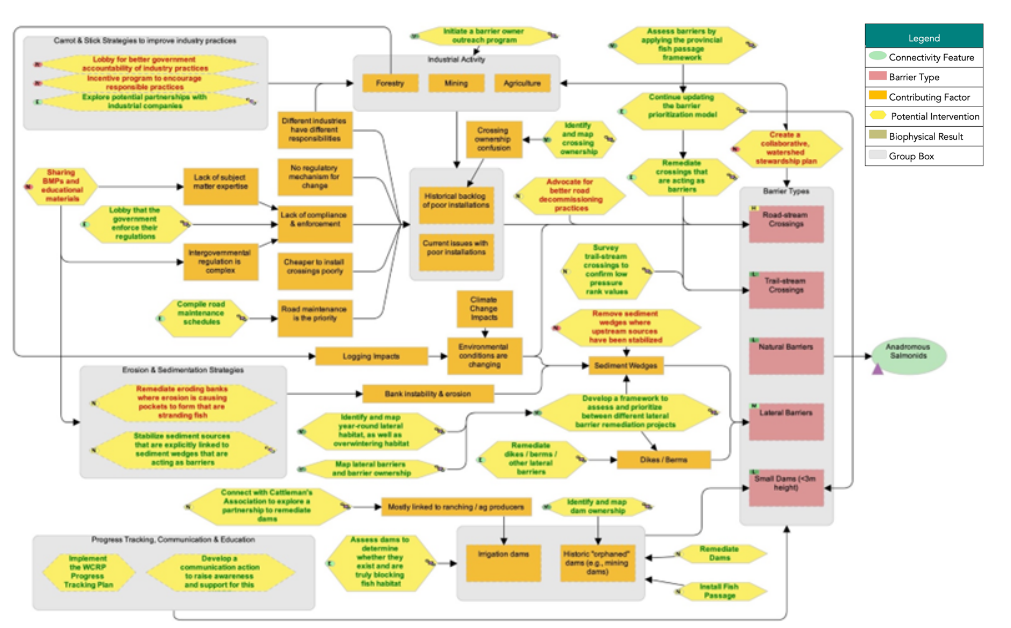
\includegraphics{images/figure3.png}

}

\caption{\label{fig-sitan}Situation analysis developed by the planning
team to identify factors that contribute to fragmentation (orange
boxes), biophysical results (brown boxes), and potential
strategies/actions to improve connectivity (yellow hexagons) for target
species in the Horsefly River watershed.}

\end{figure}

\hypertarget{goals}{%
\section*{Goals}\label{goals}}
\addcontentsline{toc}{section}{Goals}

\markright{Goals}

\hypertarget{tbl-goals}{}
\begin{longtable}[]{@{}ll@{}}
\caption{\label{tbl-goals}Goals to improve (1) spawning and rearing and
(2) overwintering habitat connectivity for target species in the
Horsefly River watershed over the lifespan of the WCRP (2021-2040). The
goals were established through discussions with the planning team and
represent the resulting desired state of connectivity in the watershed.
The goals are subject to change as more information and data are
collected over the course of the plan timeline (e.g., the current
connectivity status is updated based on barrier field
assessments).}\label{T_d4dd6_}\tabularnewline
\toprule\noalign{}
Goal \# & Goal \\
\midrule\noalign{}
\endfirsthead
\toprule\noalign{}
Goal \# & Goal \\
\midrule\noalign{}
\endhead
\bottomrule\noalign{}
\endlastfoot
1 & By 2040, the percent (\%) of total linear habitat accessible to
anadromous salmon will increase from 94\% to 96\% within the Horsefly
River watershed (i.e., reconnect at least 11.7 km of habitat). \\
2 & By 2024, the total area of overwintering habitat accessible to
Anadromous Salmon will increase by 1,500 m2 within the Horsefly River
watershed. \\
\end{longtable}

\hypertarget{strategies-actions}{%
\section*{Strategies \& Actions}\label{strategies-actions}}
\addcontentsline{toc}{section}{Strategies \& Actions}

\markright{Strategies \& Actions}

Effectiveness evaluation of identified conservation strategies and
associated actions to improve connectivity for target species in the
Horsefly River watershed. The planning team identified five broad
strategies to implement through this WCRP, 1) crossing remediation, 2)
lateral barrier remediation, 3) dam remediation, 4) barrier prevention,
and 5) communication and education. Individual actions were
qualitatively evaluated based on the anticipated effect each action will
have on realizing on-the-ground gains in connectivity. Effectiveness
ratings are based on a combination of ``Feasibility and''Impact'',
Feasibility is defined as the degree to which the project team can
implement the action within realistic constraints (financial, time,
ethical, etc.) and Impact is the degree to which the action is likely to
contribute to achieving one or more of the goals established in this
plan.

\hypertarget{strategy-1-crossing-remediation}{%
\section*{Strategy 1: Crossing
Remediation}\label{strategy-1-crossing-remediation}}
\addcontentsline{toc}{section}{Strategy 1: Crossing Remediation}

\markright{Strategy 1: Crossing Remediation}

\begin{table}

\end{table}

\hypertarget{strategy-2-lateral-barrier-remediation}{%
\section*{Strategy 2: Lateral Barrier
Remediation}\label{strategy-2-lateral-barrier-remediation}}
\addcontentsline{toc}{section}{Strategy 2: Lateral Barrier Remediation}

\markright{Strategy 2: Lateral Barrier Remediation}

\hypertarget{tbl-S2}{}
\begin{longtable}[]{@{}llllll@{}}
\caption{\label{tbl-S2}Strategy 2}\label{T_7e97d_}\tabularnewline
\toprule\noalign{}
ID & Actions & Details & Feasibility & Impact & Effectiveness \\
\midrule\noalign{}
\endfirsthead
\toprule\noalign{}
ID & Actions & Details & Feasibility & Impact & Effectiveness \\
\midrule\noalign{}
\endhead
\bottomrule\noalign{}
\endlastfoot
2.1 & Remediate dikes / berms / other lateral barriers & & High & Very
high & Effective \\
2.2 & Initiate a barrier owner outreach program & & Very high & Very
high & Very effective \\
2.3 & Knowledge Gap: Identify and map year-round lateral habitat, as
well as overwintering habitat & Explore the use of a drone to identify
lateral habitat. - Volunteers from the HRR will conduct field habitat
assessments following modules in the Pacific Streamkeepers Handbook to
assess disconnected lateral and overwintering salmon habitats in the
Horsefly watershed CNFASAR proposal: -Funding for equipment in
2022-2023, and for field transportation in 2022-2023, 2023-2024 & Very
high & Very high & Very effective \\
2.4 & Knowledge Gap: Map lateral barriers and barrier ownership & Focus
on identifying ownership of priority lateral barriers that we want to
remediate in the short-term. & Very high & Very high & Very effective \\
2.5 & Knowledge Gap: Develop a framework to assess and prioritize
between different lateral barrier remediation projects & CWF is leading
a provincial-scale analysis of the effect of rail lines on connectivity
for Anadromous Salmonids, as part of this project lateral habitat and
barrier assessments and prioritization methods will be developed. & Very
high & Very high & Very effective \\
\end{longtable}

\hypertarget{strategy-3-dam-remediation}{%
\section*{Strategy 3: Dam
Remediation}\label{strategy-3-dam-remediation}}
\addcontentsline{toc}{section}{Strategy 3: Dam Remediation}

\markright{Strategy 3: Dam Remediation}

\hypertarget{tbl-S3}{}
\begin{longtable}[]{@{}llllll@{}}
\caption{\label{tbl-S3}Strategy 3}\label{T_9252e_}\tabularnewline
\toprule\noalign{}
ID & Actions & Details & Feasibility & Impact & Effectiveness \\
\midrule\noalign{}
\endfirsthead
\toprule\noalign{}
ID & Actions & Details & Feasibility & Impact & Effectiveness \\
\midrule\noalign{}
\endhead
\bottomrule\noalign{}
\endlastfoot
3.1 & Remediate Dams & & Medium & Very high & Need more information \\
3.2 & Install Fish Passage & & Medium & High & Need more information \\
3.3 & Connect with Cattleman\textquotesingle s Association to explore a
partnership to remediate dams & This may involve exploring alternative
water management actions that would allow for the remediation of
irrigation dams. & High & Medium & Need more information \\
3.4 & Knowledge Gap: Continue updating the barrier prioritization model
& The model has been updated to reflect 2021 field assessments and
intermediate barrier review. & Very high & High & Effective \\
3.5 & Knowledge Gap: Assess dams to determine whether they exist and are
truly blocking fish habitat & Four dams were assessed during 2021 field
season; additional field assessment needed. & Very high & High &
Effective \\
3.6 & Knowledge Gap: Identify and map dam ownership & & Very high & Very
high & Very effective \\
\end{longtable}

\hypertarget{strategy-4-barrier-prevention}{%
\section*{Strategy 4: Barrier
Prevention}\label{strategy-4-barrier-prevention}}
\addcontentsline{toc}{section}{Strategy 4: Barrier Prevention}

\markright{Strategy 4: Barrier Prevention}

\hypertarget{tbl-S4}{}
\begin{longtable}[]{@{}llllll@{}}
\caption{\label{tbl-S4}Strategy 4}\label{T_8b536_}\tabularnewline
\toprule\noalign{}
ID & Actions & Details & Feasibility & Impact & Effectiveness \\
\midrule\noalign{}
\endfirsthead
\toprule\noalign{}
ID & Actions & Details & Feasibility & Impact & Effectiveness \\
\midrule\noalign{}
\endhead
\bottomrule\noalign{}
\endlastfoot
4.1 & Explore potential partnerships with industrial companies & Invite
industrial players to a workshop on how to apply crossing / lateral
barrier BMPs. BMPs could include those that minimize the need for
road-stream crossings. & Very high & High & Effective \\
4.2 & Stabilize sediment sources that are explicitly linked to sediment
wedges or erosion that are acting as barriers & This could include
numerous bank stabilization techniques, including restoring riparian
vegetation. This applies to some tributaries that have altered
confluence areas - the link needs to be made between confluence
alterations and timing of movement for juvenile fish. Local ranchers and
Cattleman\textquotesingle s association could be engaged, as well as
forestry licensees. & Very high & Medium & Need more information \\
\end{longtable}

\hypertarget{strategy-5-communication-and-education}{%
\section*{Strategy 5: Communication and
Education}\label{strategy-5-communication-and-education}}
\addcontentsline{toc}{section}{Strategy 5: Communication and Education}

\markright{Strategy 5: Communication and Education}

\hypertarget{tbl-S5}{}
\begin{longtable}[]{@{}lll@{}}
\caption{\label{tbl-S5}Strategy 5}\label{T_5e338_}\tabularnewline
\toprule\noalign{}
ID & Actions & Details \\
\midrule\noalign{}
\endfirsthead
\toprule\noalign{}
ID & Actions & Details \\
\midrule\noalign{}
\endhead
\bottomrule\noalign{}
\endlastfoot
5.1 & Implement the WCRP Progress Tracking Plan & The WCRP Progress
Tracking Plan will help the team determine if we are achieving our goals
and objectives. \\
5.2 & Develop a communication strategy to raise awareness and support
for this WCRP & This intervention includes communicating both the WCRP
and the collaborative process in developing it, as well as communicating
outcomes (e.g., barrier remediations). CNFASAR proposal: - HRR will work
with CWF to develop outreach and communications materials, including
press releases, social media content, a video, and content for their
website - With HRR, CWF will present on fish passage issues and
solutions at the annual Horsefly River Salmon Festival \\
\end{longtable}

\hypertarget{theories-of-change-objectives}{%
\section*{Theories of Change \&
Objectives}\label{theories-of-change-objectives}}
\addcontentsline{toc}{section}{Theories of Change \& Objectives}

\markright{Theories of Change \& Objectives}

Theories of Change are explicit assumptions around how the identified
actions will achieve gains in connectivity and contribute towards
reaching the goals of the plan. To develop Theories of Change, the
planning team developed explicit assumptions for each strategy which
helped to clarify the rationale used for undertaking actions and
provided an opportunity for feedback on invalid assumptions or missing
opportunities. The Theories of Change are results oriented and clearly
define the expected outcome. The following theory of change models were
developed by the WCRP planning team to ``map'' the causal (``if-then'')
progression of assumptions of how the actions within a strategy work
together to achieve project goals.

\begin{figure}

{\centering 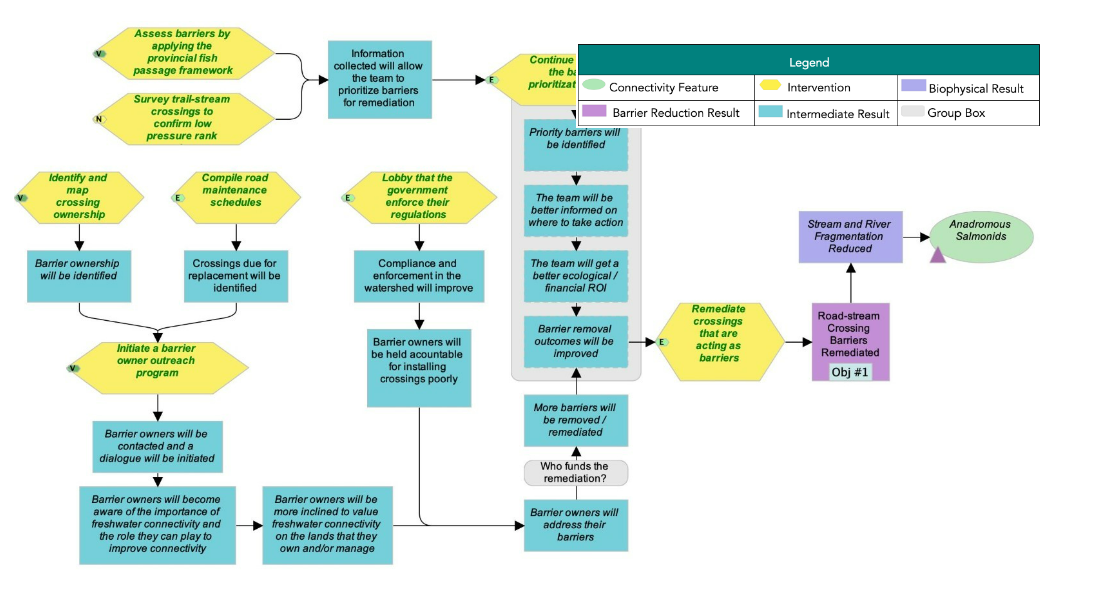
\includegraphics{images/figure4.png}

}

\caption{\label{fig-stra1}Theory of change developed by the planning
team for the actions identified under Strategy 1: Crossing Remediation
in the Horsefly River watershed.}

\end{figure}

\begin{figure}

{\centering 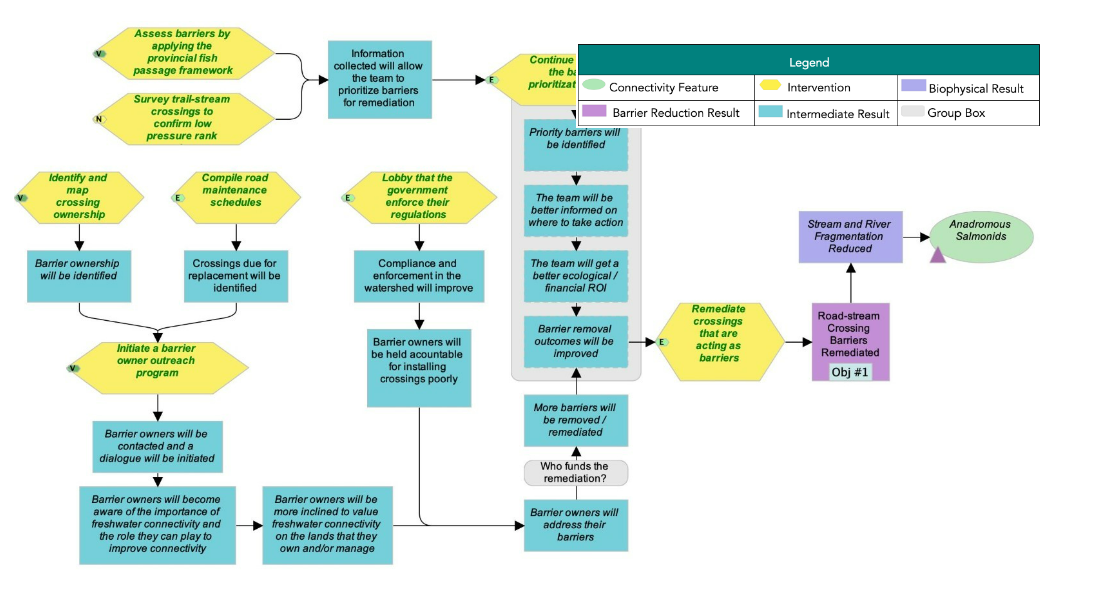
\includegraphics{images/figure4.png}

}

\caption{\label{fig-stra2}Theory of change developed by the planning
team for the actions identified under Strategy 2: Lateral Barrier
Remediation in the Horsefly River watershed.}

\end{figure}

\begin{figure}

{\centering 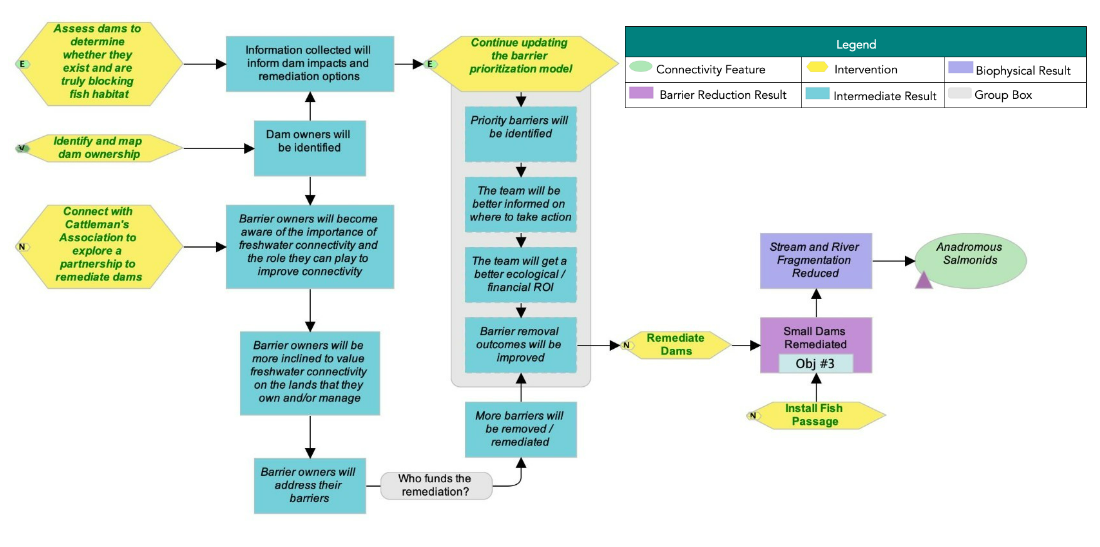
\includegraphics{images/figure6.png}

}

\caption{\label{fig-stra3}Theory of change developed by the planning
team for the actions identified under Strategy 3: Dam Remediation in the
Horsefly River watershed.}

\end{figure}

\begin{figure}

{\centering 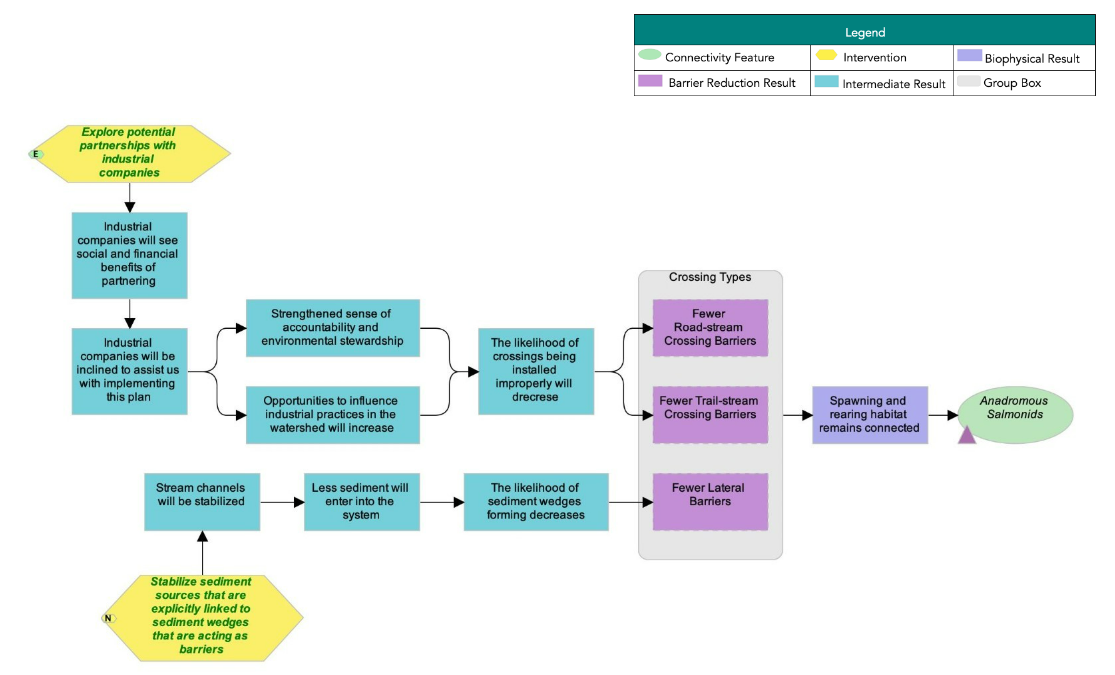
\includegraphics{images/figure7.png}

}

\caption{\label{fig-stra4}Theory of change developed by the planning
team for the actions identified under Strategy 4: Barrier Prevention in
the Horsefly River watershed.}

\end{figure}

\hypertarget{operational-plan}{%
\section*{Operational Plan}\label{operational-plan}}
\addcontentsline{toc}{section}{Operational Plan}

\markright{Operational Plan}

The operational plan represents a preliminary exercise undertaken by the
planning team to identify the potential leads, potential participants,
and estimated cost for the implementation of each action in the Horsefly
River watershed. The table below summarizes individuals, groups, or
organizations that the planning team felt could lead or participate in
the implementation of the plan and should be interpreted as the first
step in on-going planning and engagement to develop more detailed and
sophisticated action plans for each entry in the table. The individuals,
groups, and organizations listed under the ``Lead(s)'' or ``Potential
Participants'' columns are those that provisionally expressed interest
in participating in one of those roles or were suggested by the planning
team for further engagement (denoted in bold), for those that are not
members of the planning team. The leads, participants, and estimated
costs in the operational plan are not binding nor an official commitment
of resources, but rather provide a roadmap for future coordination and
engagement to work towards implementation of the WCRP.

\hypertarget{tbl-opplan}{}
\begin{longtable}[]{@{}llll@{}}
\caption{\label{tbl-opplan}Operational plan to support the
implementation of strategies and actions to improve connectivity for
target species in the Horsefly River
watershed.}\label{T_2047d_}\tabularnewline
\toprule\noalign{}
Strategy / Actions & Lead(s) {[}1{]} & Participants3 & Total Budget \\
\midrule\noalign{}
\endfirsthead
\toprule\noalign{}
Strategy / Actions & Lead(s) {[}1{]} & Participants3 & Total Budget \\
\midrule\noalign{}
\endhead
\bottomrule\noalign{}
\endlastfoot
Strategy 1: Crossing Remediation & & & \$3,666,300.00 \\
1.1 -- Remediate crossings that are acting as barriers & CWF & Horsefly
River Roundtable, Fisheries and Oceans Canada (DFO) & \$3,500,000.00 \\
1.2 -- Lobby that the government enforce their regulations & TBD & CWF,
Horsefly River Roundtable, Williams Lake First Nation (WLFN) &
\$10,000.00 \\
1.3 -- Initiate a barrier owner outreach program for locations on the
barrier remediation shortlist & HRR, CWF, DFO & & TBD \\
1.4 -- Knowledge Gap: Continue updating the barrier prioritization model
& CWF & TBD & \$100,000.00 \\
1.5 -- Knowledge Gap: conduct field assessments on updated preliminary
barrier list using the provincial fish passage framework and update
connectivity goal if additional barriers are added to the barrier
remediation shortlist & CWF & Horsefly River Roundtable, DFO &
\$50,300.00 \\
1.6 - Update longitudinal connectivity goal if additional barriers are
added to the barrier remediation shortlist & & & \\
1.7 -- Knowledge Gap: Identify and map crossing ownership for barriers
on the barrier remediation shortlist & TBD & CWF, DFO (Anthonie) &
\$1,500.00 \\
1.8 -- Knowledge Gap: Compile road maintenance schedules & DFO & CWF,
WLFN, DFO, FLNRORD & \$2,000.00 \\
1.9 -- Knowledge Gap: Survey trail-stream crossings to confirm low
pressure rating values & WLFN & CWF, DFO & \$2,500.00 \\
Strategy 2: Lateral Barrier Remediation & & & \$80,000.00 \\
2.1 -- Remediate dikes / berms / other structures that are acting as
barriers & CWF & DFO, Horsefly River Roundtable & TBD \\
2.2 -- Initiate a barrier owner outreach program & TBD & CWF, DFO &
TBD \\
2.3 -- Knowledge Gap: Identify and map year-round lateral habitat, as
well as overwintering habitat & Horsefly River Roundtable, DFO & CWF,
Northern Shuswap Tribal Council (NSTC), WLFN & \$65,000.00 \\
2.4 -- Knowledge Gap: Map lateral barriers and barrier ownership & CWF &
DFO, Horsefly River Roundtable & \$5,000.00 \\
2.5 -- Knowledge Gap: Develop a framework to assess and prioritize
between different lateral barrier remediation projects & CWF & DFO &
\$10,000.00 \\
Strategy 3: Dam Remediation & & & \$1,305,000.00 \\
3.1 - Remediate Dams & TBD & TBD & \$1,305,000.00 \\
3.2 - Install Fish Passage & TBD & TBD & TBD \\
3.3 - Connect with Cattleman\textquotesingle s Association to explore a
partnership to remediate dams & TBD & TBD & TBD \\
3.4 - Knowledge Gap: Continue updating the barrier prioritization model
& CWF & TBD & \$0.00 \\
3.5 - Knowledge Gap: Assess dams to determine whether they exist and are
truly blocking salmon habitat & HRR(?) DFO(?) CWF(?) & TBD & TBD \\
3.6 - Knowledge Gap: Identify and map dam ownership & TBD & TBD & TBD \\
Strategy 4: Barrier Prevention & & & \$110,000.00 \\
4.1 -- Explore potential partnerships with industrial companies & TBD &
CWF, DFO, Horsefly River Roundtable, WLFN & \$10,000.00 \\
4.2 -- Stabilize sediment sources that are explicitly linked to sediment
wedges or erosion that are acting as barriers & TBD & DFO &
\$100,000.00 \\
Strategy 5: Progress Tracking Plan & & & TBD \\
5.1 - Implement the WCRP Progress Tracking Plan & CWF & & TBD \\
5.2 - Develop a communication action to raise awareness and support for
this WCRP & CWF, HRR & TBD & TBD \\
Total: & & & \$5,161,300.00 \\
Fundraising total: & & & \$2,508,800 \\
Proponent/government contribution total: & & & \$2,652,500 \\
& & & \\
& & & \\
& & & \\
\end{longtable}

\hypertarget{funding-sources}{%
\section*{Funding Sources}\label{funding-sources}}
\addcontentsline{toc}{section}{Funding Sources}

\markright{Funding Sources}

\hypertarget{tbl-fund}{}
\global\setlength{\Oldarrayrulewidth}{\arrayrulewidth}

\global\setlength{\Oldtabcolsep}{\tabcolsep}

\setlength{\tabcolsep}{0pt}

\renewcommand*{\arraystretch}{1.5}



\providecommand{\ascline}[3]{\noalign{\global\arrayrulewidth #1}\arrayrulecolor[HTML]{#2}\cline{#3}}

\begin{longtable}[c]{|p{5.52in}|p{60.28in}}

\caption{\label{tbl-fund}Potential funding sources for plan implementation in the Horsefly River
watershed. The Canadian Wildlife Federation and the planning team can
coordinate proposal submission through these sources. } \\ 


\hhline{>{\arrayrulecolor[HTML]{666666}\global\arrayrulewidth=1.5pt}->{\arrayrulecolor[HTML]{666666}\global\arrayrulewidth=1.5pt}-}

\multicolumn{1}{>{\cellcolor[HTML]{008270}\raggedright}m{\dimexpr 5.52in+0\tabcolsep}}{\textcolor[HTML]{FFFFFF}{\fontsize{11}{11}\selectfont{Funding\ Source}}} & \multicolumn{1}{>{\cellcolor[HTML]{008270}\raggedright}m{\dimexpr 60.28in+0\tabcolsep}}{\textcolor[HTML]{FFFFFF}{\fontsize{11}{11}\selectfont{Spending\ Restrictions\ and\ Other\ Consideration}}} \\

\noalign{\global\arrayrulewidth 0pt}\arrayrulecolor[HTML]{000000}

\hhline{>{\arrayrulecolor[HTML]{666666}\global\arrayrulewidth=1.5pt}->{\arrayrulecolor[HTML]{666666}\global\arrayrulewidth=1.5pt}-}\endhead



\multicolumn{1}{>{\raggedright}m{\dimexpr 5.52in+0\tabcolsep}}{\textcolor[HTML]{000000}{\fontsize{11}{11}\selectfont{Land\ Based\ Investment\ Strategy}}} & \multicolumn{1}{>{\raggedright}m{\dimexpr 60.28in+0\tabcolsep}}{\textcolor[HTML]{000000}{\fontsize{11}{11}\selectfont{Assessment\ and\ remediation\ of\ fish\ passage\ using\ provincial\ strategic\ approach.\ Primarily\ for\ remediation\ of\ Ministry-owned/orphaned\ barriers\ on\ forest\ service\ roads.}}} \\

\noalign{\global\arrayrulewidth 0pt}\arrayrulecolor[HTML]{000000}





\multicolumn{1}{>{\raggedright}m{\dimexpr 5.52in+0\tabcolsep}}{\textcolor[HTML]{000000}{\fontsize{11}{11}\selectfont{Environmental\ Enhancement\ Fund}}} & \multicolumn{1}{>{\raggedright}m{\dimexpr 60.28in+0\tabcolsep}}{\textcolor[HTML]{000000}{\fontsize{11}{11}\selectfont{Fish\ and\ wildlife\ passage\ improvements\ and\ restoration\ at\ stream\ and\ animal\ crossings\ at\ MOTI\ roads\ including\ culvert\ retrofits\ and\ replacement\ to\ restore\ Pacific\ salmon\ and\ trout\ access,\ and\ wildlife\ tunnels.\ Primarily\ for\ crossings\ linked\ to\ highway\ infrastructure.}}} \\

\noalign{\global\arrayrulewidth 0pt}\arrayrulecolor[HTML]{000000}





\multicolumn{1}{>{\raggedright}m{\dimexpr 5.52in+0\tabcolsep}}{\textcolor[HTML]{000000}{\fontsize{11}{11}\selectfont{Community\ Salmon\ Program}}} & \multicolumn{1}{>{\raggedright}m{\dimexpr 60.28in+0\tabcolsep}}{\textcolor[HTML]{000000}{\fontsize{11}{11}\selectfont{For\ projects\ supporting\ the\ protection,\ conservation\ and\ enhancement\ or\ rehabilitation\ of\ Pacific\ salmonids\ and\ their\ habitat.\ Funding\ for\ volunteer\ and\ not-for-profit\ community-based\ groups.\ Applicant\ must\ have\ a\ significant\ volunteer\ component\ to\ their\ group\ and\ to\ the\ project.\ Requires\ 50\%\ match\ for\ funding\ (volunteer,\ in-kind,\ donation\ or\ other\ grants).\ }}} \\

\noalign{\global\arrayrulewidth 0pt}\arrayrulecolor[HTML]{000000}





\multicolumn{1}{>{\raggedright}m{\dimexpr 5.52in+0\tabcolsep}}{\textcolor[HTML]{000000}{\fontsize{11}{11}\selectfont{Southern\ Boundary\ Restoration\ and\ Enhancement\ Fund}}} & \multicolumn{1}{>{\raggedright}m{\dimexpr 60.28in+0\tabcolsep}}{\textcolor[HTML]{000000}{\fontsize{11}{11}\selectfont{Supports\ 3\ activities:\ (1)\ develop\ improved\ information\ for\ resource\ management;\ (2)\ Rehabilitate\ and\ restore\ marine\ and\ freshwater\ habitat;\ and\ (3)\ enhance\ wild\ stock\ production\ through\ low\ technology\ techniques.\ Emphasis\ for\ funding\ is\ on\ stocks\ of\ conservation\ concern,\ particularly\ those\ contributing\ to\ a\ fishery\ and\ stocks\ of\ bilateral\ fishery\ relevance.}}} \\

\noalign{\global\arrayrulewidth 0pt}\arrayrulecolor[HTML]{000000}





\multicolumn{1}{>{\raggedright}m{\dimexpr 5.52in+0\tabcolsep}}{\textcolor[HTML]{000000}{\fontsize{11}{11}\selectfont{Habitat\ Conservation\ Trust\ Foundation\ Enhancement\ and\ Restoration\ Grants}}} & \multicolumn{1}{>{\raggedright}m{\dimexpr 60.28in+0\tabcolsep}}{\textcolor[HTML]{000000}{\fontsize{11}{11}\selectfont{Projects\ that\ focus\ on\ freshwater\ wild\ fish,\ native\ wildlife\ species\ and\ their\ habitats,\ have\ the\ potential\ to\ achieve\ a\ significant\ conservation\ outcome,\ while\ maintaining\ or\ enhancing\ opportunities\ for\ fishing,\ hunting,\ trapping,\ wildlife\ viewing\ and\ associated\ outdoor\ recreational\ activities.\ Primary\ focus\ is\ on\ provincially\ managed\ fisheries\ such\ as\ Steelhead\ and\ Westslope\ Cutthroat\ Trout.\ Requires\ 50\%\ funding\ match.}}} \\

\noalign{\global\arrayrulewidth 0pt}\arrayrulecolor[HTML]{000000}





\multicolumn{1}{>{\raggedright}m{\dimexpr 5.52in+0\tabcolsep}}{\textcolor[HTML]{000000}{\fontsize{11}{11}\selectfont{Environmental\ Damages\ Fund}}} & \multicolumn{1}{>{\raggedright}m{\dimexpr 60.28in+0\tabcolsep}}{\textcolor[HTML]{000000}{\fontsize{11}{11}\selectfont{Direct\ funds\ received\ from\ fines,\ court\ orders\ and\ voluntary\ payments\ to\ priority\ projects\ that\ will\ benefit\ Canada’s\ natural\ environment,\ under\ 4\ categories\ of\ improvement\ (in\ order\ of\ preference):\ (1)\ restoration,\ (2)\ environmental\ quality\ improvement,\ (3)\ research\ and\ development,\ and\ (4)\ education\ and\ awareness.}}} \\

\noalign{\global\arrayrulewidth 0pt}\arrayrulecolor[HTML]{000000}





\multicolumn{1}{>{\raggedright}m{\dimexpr 5.52in+0\tabcolsep}}{\textcolor[HTML]{000000}{\fontsize{11}{11}\selectfont{Habitat\ Stewardship\ Program\ for\ Aquatic\ Species\ at\ Risk}}} & \multicolumn{1}{>{\raggedright}m{\dimexpr 60.28in+0\tabcolsep}}{\textcolor[HTML]{000000}{\fontsize{11}{11}\selectfont{Program\ for\ non-profits,\ Indigenous\ governments,\ academic\ institutions\ for\ activities\ that\ align\ with\ recovery\ actions\ identified\ in\ SARA\ recovery\ documents\ and/or\ COSEWIC\ assessment\ documents.\ Project\ must\ address\ one\ or\ more\ of\ 3\ broad\ categories:\ (1)\ Important\ habitat\ for\ aquatic\ species\ at\ risk\ is\ improved\ and/or\ managed\ to\ meet\ their\ recovery\ needs;\ (2)\ Threats\ to\ aquatic\ species\ at\ risk\ and/or\ their\ habitat\ are\ stopped,\ removed,\ and/or\ mitigated;\ (3)\ Collaboration\ and\ partnerships\ support\ the\ conservation\ and\ recovery\ of\ aquatic\ species\ at\ risk.\ Limited\ to\ at-risk\ species\ listed\ under\ COSEWIC\ and/or\ SARA\ as\ threatened,\ endangered\ or\ special\ concern.\ }}} \\

\noalign{\global\arrayrulewidth 0pt}\arrayrulecolor[HTML]{000000}





\multicolumn{1}{>{\raggedright}m{\dimexpr 5.52in+0\tabcolsep}}{\textcolor[HTML]{000000}{\fontsize{11}{11}\selectfont{Canada\ Nature\ Fund\ for\ Aquatic\ Species\ at\ Risk}}} & \multicolumn{1}{>{\raggedright}m{\dimexpr 60.28in+0\tabcolsep}}{\textcolor[HTML]{000000}{\fontsize{11}{11}\selectfont{Funding\ program\ aimed\ at\ addressing\ priority\ threats\ for\ aquatic\ species\ at\ risk\ listed\ as\ endangered,\ threatened\ or\ Special\ Concern\ by\ COSEWIC,\ as\ they\ align\ with\ existing\ federal,\ provincial\ or\ other\ local\ recovery\ plans.\ Limited\ to\ species\ in\ the\ Columbia\ and\ Fraser\ basins\ in\ BC,\ among\ other\ priority\ areas\ across\ Canada.\ Focus\ on\ multi-year,\ multi-partner\ initiatives\ that\ apply\ an\ ecosystem\ or\ multi-species\ approach\ and\ create\ a\ legacy\ by\ enabling\ recovery\ actions\ that\ carry\ beyond\ the\ life\ of\ the\ funding\ program.\ Amounts\ from\ \$100K-\$1M\ available\ per\ year.}}} \\

\noalign{\global\arrayrulewidth 0pt}\arrayrulecolor[HTML]{000000}





\multicolumn{1}{>{\raggedright}m{\dimexpr 5.52in+0\tabcolsep}}{\textcolor[HTML]{000000}{\fontsize{11}{11}\selectfont{BC\ Salmon\ Restoration\ and\ Innovation\ Fund}}} & \multicolumn{1}{>{\raggedright}m{\dimexpr 60.28in+0\tabcolsep}}{\textcolor[HTML]{000000}{\fontsize{11}{11}\selectfont{Funding\ for\ Indigenous\ enterprises,\ academia,\ industry\ associations,\ stewardship\ groups\ and\ commercial\ groups\ to\ support\ initiatives\ that\ support\ the\ protection\ and\ restoration\ of\ wild\ Pacific\ salmon\ and\ other\ BC\ fish\ stocks\ or\ ensure\ fish\ and\ seafood\ sector\ in\ BC\ is\ environmentally\ and\ economically\ sustainable.\ Five\ main\ priorities\ including\ species\ of\ concern\ rebuilding\ through\ habitat\ restoration\ with\ priority\ for\ projects\ that\ are\ part\ of\ a\ watershed-scale\ restoration\ plan/prioritization\ effort;\ build\ on\ successful\ previous\ restoration\ efforts;\ focus\ on\ critical\ habitat\ and/or\ the\ rehabilitation\ of\ natural\ ecosystem\ processes.}}} \\

\noalign{\global\arrayrulewidth 0pt}\arrayrulecolor[HTML]{000000}





\multicolumn{1}{>{\raggedright}m{\dimexpr 5.52in+0\tabcolsep}}{\textcolor[HTML]{000000}{\fontsize{11}{11}\selectfont{Aboriginal\ Fund\ for\ Species\ at\ Risk}}} & \multicolumn{1}{>{\raggedright}m{\dimexpr 60.28in+0\tabcolsep}}{\textcolor[HTML]{000000}{\fontsize{11}{11}\selectfont{Program\ for\ Indigenous\ groups\ for\ activities\ that\ align\ with\ recovery\ actions\ identified\ in\ SARA\ recovery\ documents\ and/or\ COSEWIC\ assessment\ documents\ for\ species\ listed\ as\ Endangered,\ Threatened,\ or\ Special\ Concern\ by\ SARA\ or\ COSEWIC.\ Project\ must\ address\ one\ or\ more\ of\ 4\ broad\ categories:\ (1)\ Habitat\ for\ species\ at\ risk\ is\ improved\ and/or\ managed\ to\ meet\ their\ recovery\ needs;\ (2)\ Threats\ to\ species\ at\ risk\ and/or\ their\ habitat\ are\ stopped,\ removed\ and/or\ mitigated;\ (3)\ Collaboration,\ information\ sharing\ and\ partnership\ between\ Indigenous\ communities,\ governments\ and\ organizations\ and\ other\ interested\ parties\ (e.g.\ federal/provincial/territorial\ governments,\ academia,\ industry,\ private\ sector)\ is\ enhanced;\ and\ (4)\ Capacity\ within\ Indigenous\ communities,\ to\ lead\ in\ the\ stewardship\ of\ species\ at\ risk\ and\ contribute\ to\ broader\ SARA\ implementation,\ is\ strengthened.\ }}} \\

\noalign{\global\arrayrulewidth 0pt}\arrayrulecolor[HTML]{000000}





\multicolumn{1}{>{\raggedright}m{\dimexpr 5.52in+0\tabcolsep}}{\textcolor[HTML]{000000}{\fontsize{11}{11}\selectfont{Federal\ Gas\ Tax\ Fund\ -\ Community\ Works\ Fund}}} & \multicolumn{1}{>{\raggedright}m{\dimexpr 60.28in+0\tabcolsep}}{\textcolor[HTML]{000000}{\fontsize{11}{11}\selectfont{Funding\ available\ to\ local\ governments\ from\ federal\ gas\ tax,\ with\ funds\ to\ be\ allocated\ for\ a\ variety\ of\ municipal\ projects/initiatives,\ including\ local\ roads/bridges\ and\ disaster\ mitigation.}}} \\

\noalign{\global\arrayrulewidth 0pt}\arrayrulecolor[HTML]{000000}





\multicolumn{1}{>{\raggedright}m{\dimexpr 5.52in+0\tabcolsep}}{\textcolor[HTML]{000000}{\fontsize{11}{11}\selectfont{Disaster\ Mitigation\ and\ Adaptation\ Fund}}} & \multicolumn{1}{>{\raggedright}m{\dimexpr 60.28in+0\tabcolsep}}{\textcolor[HTML]{000000}{\fontsize{11}{11}\selectfont{For\ those\ projects\ where\ flood\ risk\ is\ high:\ Funding\ available\ to\ local,\ regional\ and\ provincial\ governments,\ private\ sector,\ non-profit\ organizations,\ and\ Indigenous\ groups\ for\ projects\ aimed\ at\ reducing\ the\ socio-economic,\ environmental\ and\ cultural\ impacts\ triggered\ by\ natural\ hazards\ and\ extreme\ weather\ events\ and\ taking\ into\ consideration\ current\ and\ future\ impacts\ of\ climate\ change\ in\ communities\ and\ infrastructure\ at\ high\ risk.\ Includes\ both\ new\ construction\ of\ public\ infrastructure\ and\ modification/reinforcement\ of\ existing\ infrastructure.\ Projects\ must\ have\ a\ minimum\ of\ \$20\ M\ in\ eligible\ expenditures\ and\ can\ be\ bundled\ together.}}} \\

\noalign{\global\arrayrulewidth 0pt}\arrayrulecolor[HTML]{000000}





\multicolumn{1}{>{\raggedright}m{\dimexpr 5.52in+0\tabcolsep}}{\textcolor[HTML]{000000}{\fontsize{11}{11}\selectfont{Community\ Gaming\ Grants}}} & \multicolumn{1}{>{\raggedright}m{\dimexpr 60.28in+0\tabcolsep}}{\textcolor[HTML]{000000}{\fontsize{11}{11}\selectfont{Funding\ for\ non-profit\ organizations\ (check\ funding\ program\ guidelines\ for\ specific\ eligibility\ requirements)\ for\ programs\ that\ help\ to\ protect\ and\ improve\ the\ environment\ by:\ (1)\ Conserving\ or\ revitalizing\ local\ ecosystems,\ (2)\ Reducing\ greenhouse\ gas\ emissions,\ (3)\ Providing\ community\ education\ or\ engagement\ opportunities\ related\ to\ the\ environment\ and\ agriculture\ or\ (4)\ Supporting\ the\ welfare\ of\ domestic\ animals\ and/or\ wildlife.\ Grants\ range\ from\ \$100K-250K\ per\ year.}}} \\

\noalign{\global\arrayrulewidth 0pt}\arrayrulecolor[HTML]{000000}





\multicolumn{1}{>{\raggedright}m{\dimexpr 5.52in+0\tabcolsep}}{\textcolor[HTML]{000000}{\fontsize{11}{11}\selectfont{Sitka\ Foundation}}} & \multicolumn{1}{>{\raggedright}m{\dimexpr 60.28in+0\tabcolsep}}{\textcolor[HTML]{000000}{\fontsize{11}{11}\selectfont{Funding\ for\ registered\ charities,\ universities,\ and\ government\ agencies\ (qualified\ Canadian\ organizations)\ for\ projects\ related\ to\ coastline\ and\ watershed\ conservation\ and\ climate\ change\ in\ 4\ key\ areas:\ (1)\ land,\ water,\ and\ ocean\ conservation,\ (2)\ scientific\ research\ for\ nature\ and\ the\ environment,\ (3)\ \ public\ engagement\ around\ the\ importance\ of\ a\ healthy\ environment,\ (4)\ innovative\ conservation\ efforts\ in\ Canadian\ communities,\ at\ the\ local,\ provincial,\ and\ federal\ levels}}} \\

\noalign{\global\arrayrulewidth 0pt}\arrayrulecolor[HTML]{000000}





\multicolumn{1}{>{\raggedright}m{\dimexpr 5.52in+0\tabcolsep}}{\textcolor[HTML]{000000}{\fontsize{11}{11}\selectfont{TULA\ Foundation}}} & \multicolumn{1}{>{\raggedright}m{\dimexpr 60.28in+0\tabcolsep}}{\textcolor[HTML]{000000}{\fontsize{11}{11}\selectfont{Supports\ various\ environmental\ programs\ of\ interest\ to\ the\ Foundation\ on\ a\ case-by-case\ basis.}}} \\

\noalign{\global\arrayrulewidth 0pt}\arrayrulecolor[HTML]{000000}





\multicolumn{1}{>{\raggedright}m{\dimexpr 5.52in+0\tabcolsep}}{\textcolor[HTML]{000000}{\fontsize{11}{11}\selectfont{Vancouver\ Foundation}}} & \multicolumn{1}{>{\raggedright}m{\dimexpr 60.28in+0\tabcolsep}}{\textcolor[HTML]{000000}{\fontsize{11}{11}\selectfont{Granting\ agency\ for\ community,\ social\ and\ environmental\ initiatives\ for\ qualified\ Canadian\ organizations\ (charitable\ organizations,\ universities,\ government\ agencies).\ Granting\ programs\ change\ on\ an\ annual\ basis.}}} \\

\noalign{\global\arrayrulewidth 0pt}\arrayrulecolor[HTML]{000000}





\multicolumn{1}{>{\raggedright}m{\dimexpr 5.52in+0\tabcolsep}}{\textcolor[HTML]{000000}{\fontsize{11}{11}\selectfont{BC\ Conservation\ Foundation\ Small\ Project\ Fund}}} & \multicolumn{1}{>{\raggedright}m{\dimexpr 60.28in+0\tabcolsep}}{\textcolor[HTML]{000000}{\fontsize{11}{11}\selectfont{Funding\ available\ to\ Non-profits,\ fish\ and\ wildlife\ clubs\ (sportsmen’s\ associations),\ businesses,\ local/regional\ governments,\ public\ organizations\ and\ First\ Nations\ for\ projects\ with\ demonstrated\ positive\ impact\ for\ fish,\ wildlife\ and\ habitat,\ including\ outreach\ programs.\ Preference\ given\ to\ projects\ where\ BCCF\ is\ not\ the\ sole\ funder.}}} \\

\noalign{\global\arrayrulewidth 0pt}\arrayrulecolor[HTML]{000000}





\multicolumn{1}{>{\raggedright}m{\dimexpr 5.52in+0\tabcolsep}}{\textcolor[HTML]{000000}{\fontsize{11}{11}\selectfont{Real\ Estate\ Foundation\ of\ BC\ General\ Grants}}} & \multicolumn{1}{>{\raggedright}m{\dimexpr 60.28in+0\tabcolsep}}{\textcolor[HTML]{000000}{\fontsize{11}{11}\selectfont{Funding\ for\ First\ Nations,\ charities\ and\ societies,\ non-governmental\ organizations,\ universities\ and\ colleges,\ trade\ associations,\ local\ and\ regional\ governments,\ and\ social\ enterprises\ registered\ as\ C3s\ for\ sustainable\ land\ use\ and\ real\ estate\ practices\ in\ BC.\ Funds\ up\ to\ 50\%\ of\ cash\ portion\ of\ a\ project.}}} \\

\noalign{\global\arrayrulewidth 0pt}\arrayrulecolor[HTML]{000000}

\hhline{>{\arrayrulecolor[HTML]{666666}\global\arrayrulewidth=1.5pt}->{\arrayrulecolor[HTML]{666666}\global\arrayrulewidth=1.5pt}-}



\end{longtable}



\arrayrulecolor[HTML]{000000}

\global\setlength{\arrayrulewidth}{\Oldarrayrulewidth}

\global\setlength{\tabcolsep}{\Oldtabcolsep}

\renewcommand*{\arraystretch}{1}

\bookmarksetup{startatroot}

\hypertarget{references}{%
\chapter*{References}\label{references}}
\addcontentsline{toc}{chapter}{References}

\markboth{References}{References}

\hypertarget{refs}{}
\begin{CSLReferences}{1}{0}
\leavevmode\vadjust pre{\hypertarget{ref-DFO1991-tl}{}}%
DFO. 1991. \emph{Fish Habitat Inventory and Information Program - Stream
Summary Information.} DFO.

\leavevmode\vadjust pre{\hypertarget{ref-MEC2018-tl}{}}%
Ltd., Masse Environmental Consultants. 2018. \emph{Fish Habitat
Confirmation Assessments Horsefly River Watershed. Prepared for Ministry
of Environment \& Climate Change Strategy.} Masse Environmental
Consultants Ltd.

\leavevmode\vadjust pre{\hypertarget{ref-Mazany-Wright2021-rz}{}}%
Mazany-Wright, N, S M Norris, N W R Lapointe, and B Rebellato. 2021a.
{``A Freshwater Connectivity Modelling Framework to Support Barrier
Prioritization and Remediation in British Columbia.''} \emph{Canadian
Wildlife Federation}.

\leavevmode\vadjust pre{\hypertarget{ref-Mazany-Wright2021-do}{}}%
---------. 2021b. {``Fish Passage Restoration Initiative Target
Watershed Selection Process: Technical Documentation.''} \emph{Canadian
Wildlife Federation}.

\leavevmode\vadjust pre{\hypertarget{ref-Mazany-Wright2021-hs}{}}%
Mazany-Wright, N, J Noseworthy, S Sra, S M Norris, and N W Lapointe.
2021. {``Breaking down Barriers: A Practitioners' Guide to Watershed
Connectivity Remediation Planning.''} \emph{Canadian Wildlife
Federation}.

\leavevmode\vadjust pre{\hypertarget{ref-WLFN2021Patterns}{}}%
Nation., Williams Lake First. 2021. \emph{Secwepemc Land Use Patterns.}
https://www.wlfn.ca/about-wlfn/history/.

\leavevmode\vadjust pre{\hypertarget{ref-XFN2021History}{}}%
Nation., Xatśūll First. 2021. {``Traditional History.''} \emph{XFN}.

\leavevmode\vadjust pre{\hypertarget{ref-PSF2020-tl}{}}%
Pacific-Salmon-Foundation. 2020. \emph{Methods for Assessing Status and
Trends in Pacific Salmon Conservation Units and Their Freshwater
Habitats. The Pacific Salmon Foundation, Vancouver, British Columbia.}
PSF.

\leavevmode\vadjust pre{\hypertarget{ref-Seliger2018-be}{}}%
Seliger, Carina, and Bernhard Zeiringer. 2018. {``River Connectivity,
Habitat Fragmentation and Related Restoration Measures,''} 171--86.

\leavevmode\vadjust pre{\hypertarget{ref-Wilson1998-kb}{}}%
Wilson, I. R., K. Twohig, and B. Dahlstrom. 1998. \emph{Archaeological
Overview Assessment Northern Secwepemc Traditional Territory.}
https://www2.gov.bc.ca/assets/gov/farming-natural-resources-and-industry/natural-resource-use/archaeology/forms-publications/aoa\_-\_williams\_lake\_-\_northern\_secwepemc\_traditional\_territory\_-\_1998\_report.pdf.

\end{CSLReferences}

\cleardoublepage
\phantomsection
\addcontentsline{toc}{part}{Appendices}
\appendix

\hypertarget{appendix-a}{%
\chapter*{Appendix A}\label{appendix-a}}
\addcontentsline{toc}{chapter}{Appendix A}

\markboth{Appendix A}{Appendix A}

\hypertarget{modelled-anadromous-salmon-habitat-maps}{%
\section*{Modelled Anadromous Salmon Habitat
Maps}\label{modelled-anadromous-salmon-habitat-maps}}
\addcontentsline{toc}{section}{Modelled Anadromous Salmon Habitat Maps}

\markright{Modelled Anadromous Salmon Habitat Maps}

High-resolution PDF maps of the Horsefly River watershed and model
results can be accessed
\href{https://github.com/smnorris/bcfishpass/tree/main/wcrp/pdfs}{here}.
The watershed is divided into multiple maps sheets to allow for detailed
examination of modelled spawning and rearing habitat, multiple barrier
types, and priority barriers identified through this planning process.
The locations of WCRP priority barriers and associated map sheet numbers
are shown below. In each individual map sheet, priority barriers are
symbolized using the following notation:

\begin{figure}

{\centering 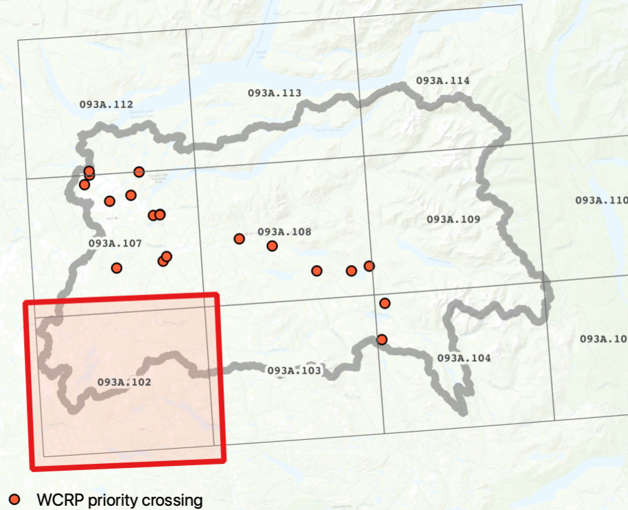
\includegraphics{images/figure8.png}

}

\caption{\label{fig-over}Horsefly River watershed overview map
identifying the portions of the watershed covered by each map sheet
(grey squares) and the prioritized barriers on the intermediate barrier
list (orange points; see Appendix B).}

\end{figure}

\hypertarget{connectivity-status-assessment-methods}{%
\section*{Connectivity Status Assessment
Methods}\label{connectivity-status-assessment-methods}}
\addcontentsline{toc}{section}{Connectivity Status Assessment Methods}

\markright{Connectivity Status Assessment Methods}

The connectivity status assessment for anadromous salmonids in the
Horsefly River watershed builds on existing connectivity modelling work
undertaken by the BC Fish Passage Technical Working Group, resulting in
a flexible, customizable open-source spatial model called
``bcfishpass''. The model spatially locates known and modelled barriers
to fish passage, identifies potential spawning and rearing habitat for
target species, and estimates the amount of habitat that is currently
accessible to target species. The model uses an adapted version of the
Intrinsic Potential (IP) fish habitat modelling framework (see Sheer et
al.~2009 for an overview of the IP framework). The habitat model uses
two geomorphic characteristics of the stream network --- channel
gradient and mean annual discharge --- to identify potential spawning
habitat and rearing habitat for each target species. The habitat model
does not attempt to definitively map each habitat type nor estimate
habitat quality, but rather identifies stream segments that have high
potential to support spawning or rearing habitat for each species based
on the geomorphic characteristics of the segment. For more details on
the connectivity and habitat model structure and parameters, please see
Mazany-Wright, Norris, et al. (2021a). The variables and thresholds used
to model potential spawning and rearing habitat for each target species
are summarized in Table 15. The quantity of modelled habitat for each
species was aggregated for each habitat type and represents a linear
measure of potential habitat. To recognize the rearing value provided by
features represented by polygons for certain species (e.g., wetlands for
Coho Salmon and lakes for Sockeye Salmon) a multiplier of 1.5x the
length of the stream segments flowing through the polygons was applied.

\hypertarget{tbl-param}{}
\global\setlength{\Oldarrayrulewidth}{\arrayrulewidth}

\global\setlength{\Oldtabcolsep}{\tabcolsep}

\setlength{\tabcolsep}{0pt}

\renewcommand*{\arraystretch}{1.5}



\providecommand{\ascline}[3]{\noalign{\global\arrayrulewidth #1}\arrayrulecolor[HTML]{#2}\cline{#3}}

\begin{longtable}[c]{|p{1.43in}|p{3.34in}|p{8.40in}|p{3.09in}|p{3.03in}|p{1.94in}|p{1.33in}}

\caption{\label{tbl-param}Additional Key Actors in the Horsefly River watershed. Key Actors are
the individuals, groups, and/or organizations, outside of the planning
team, with influence and relevant experience in the watershed, whose
engagement will be critical for the successful implementation of this
WCRP. } \\ 


\hhline{>{\arrayrulecolor[HTML]{666666}\global\arrayrulewidth=1.5pt}->{\arrayrulecolor[HTML]{666666}\global\arrayrulewidth=1.5pt}->{\arrayrulecolor[HTML]{666666}\global\arrayrulewidth=1.5pt}->{\arrayrulecolor[HTML]{666666}\global\arrayrulewidth=1.5pt}->{\arrayrulecolor[HTML]{666666}\global\arrayrulewidth=1.5pt}->{\arrayrulecolor[HTML]{666666}\global\arrayrulewidth=1.5pt}->{\arrayrulecolor[HTML]{666666}\global\arrayrulewidth=1.5pt}-}

\multicolumn{1}{>{\cellcolor[HTML]{008270}\raggedright}m{\dimexpr 1.43in+0\tabcolsep}}{\textcolor[HTML]{FFFFFF}{\fontsize{11}{11}\selectfont{Species}}} & \multicolumn{1}{>{\cellcolor[HTML]{008270}\raggedright}m{\dimexpr 3.34in+0\tabcolsep}}{\textcolor[HTML]{FFFFFF}{\fontsize{11}{11}\selectfont{Channel\ Gradient\ (\%)}}} & \multicolumn{1}{>{\cellcolor[HTML]{008270}\raggedright}m{\dimexpr 8.4in+0\tabcolsep}}{\textcolor[HTML]{FFFFFF}{\fontsize{11}{11}\selectfont{Mean\ annual\ discharge\ (m3/s)}}} & \multicolumn{1}{>{\cellcolor[HTML]{008270}\raggedright}m{\dimexpr 3.09in+0\tabcolsep}}{\textcolor[HTML]{FFFFFF}{\fontsize{11}{11}\selectfont{Channel\ gradient\ (\%)}}} & \multicolumn{1}{>{\cellcolor[HTML]{008270}\raggedright}m{\dimexpr 3.03in+0\tabcolsep}}{\textcolor[HTML]{FFFFFF}{\fontsize{11}{11}\selectfont{Mean\ Annual\ discharge\ (m3/s)}}} & \multicolumn{1}{>{\cellcolor[HTML]{008270}\raggedright}m{\dimexpr 1.94in+0\tabcolsep}}{\textcolor[HTML]{FFFFFF}{\fontsize{11}{11}\selectfont{Minimum\ Lake\ area\ (ha)}}} & \multicolumn{1}{>{\cellcolor[HTML]{008270}\raggedright}m{\dimexpr 1.33in+0\tabcolsep}}{\textcolor[HTML]{FFFFFF}{\fontsize{11}{11}\selectfont{Multiplier\ (1.5x)}}} \\

\noalign{\global\arrayrulewidth 0pt}\arrayrulecolor[HTML]{000000}

\hhline{>{\arrayrulecolor[HTML]{666666}\global\arrayrulewidth=1.5pt}->{\arrayrulecolor[HTML]{666666}\global\arrayrulewidth=1.5pt}->{\arrayrulecolor[HTML]{666666}\global\arrayrulewidth=1.5pt}->{\arrayrulecolor[HTML]{666666}\global\arrayrulewidth=1.5pt}->{\arrayrulecolor[HTML]{666666}\global\arrayrulewidth=1.5pt}->{\arrayrulecolor[HTML]{666666}\global\arrayrulewidth=1.5pt}->{\arrayrulecolor[HTML]{666666}\global\arrayrulewidth=1.5pt}-}\endhead



\multicolumn{1}{>{\raggedright}m{\dimexpr 1.43in+0\tabcolsep}}{\textcolor[HTML]{000000}{\fontsize{11}{11}\selectfont{Chinook\ Salmon}}} & \multicolumn{1}{>{\raggedright}m{\dimexpr 3.34in+0\tabcolsep}}{\textcolor[HTML]{000000}{\fontsize{11}{11}\selectfont{0-3}}} & \multicolumn{1}{>{\raggedright}m{\dimexpr 8.4in+0\tabcolsep}}{\textcolor[HTML]{000000}{\fontsize{11}{11}\selectfont{0.46-322.5}}} & \multicolumn{1}{>{\raggedright}m{\dimexpr 3.09in+0\tabcolsep}}{\textcolor[HTML]{000000}{\fontsize{11}{11}\selectfont{0-5}}} & \multicolumn{1}{>{\raggedright}m{\dimexpr 3.03in+0\tabcolsep}}{\textcolor[HTML]{000000}{\fontsize{11}{11}\selectfont{0.28-100}}} & \multicolumn{1}{>{\raggedright}m{\dimexpr 1.94in+0\tabcolsep}}{\textcolor[HTML]{000000}{\fontsize{11}{11}\selectfont{}}} & \multicolumn{1}{>{\raggedright}m{\dimexpr 1.33in+0\tabcolsep}}{\textcolor[HTML]{000000}{\fontsize{11}{11}\selectfont{}}} \\

\noalign{\global\arrayrulewidth 0pt}\arrayrulecolor[HTML]{000000}





\multicolumn{1}{>{\raggedright}m{\dimexpr 1.43in+0\tabcolsep}}{\textcolor[HTML]{000000}{\fontsize{11}{11}\selectfont{}}} & \multicolumn{1}{>{\raggedright}m{\dimexpr 3.34in+0\tabcolsep}}{\textcolor[HTML]{000000}{\fontsize{11}{11}\selectfont{(Busch\ et\ al.\ 2011,\ Cooney\ and\ Holzer\ 2006)}}} & \multicolumn{1}{>{\raggedright}m{\dimexpr 8.4in+0\tabcolsep}}{\textcolor[HTML]{000000}{\fontsize{11}{11}\selectfont{(Bjornn\ and\ Reiser\ 1991,\ Neuman\ and\ Newcombe\ 1977,\ Woll\ et\ al.\ 2017,\ Roberge\ et\ al.\ 2002,\ Raleigh\ and\ Miller\ 1986)}}} & \multicolumn{1}{>{\raggedright}m{\dimexpr 3.09in+0\tabcolsep}}{\textcolor[HTML]{000000}{\fontsize{11}{11}\selectfont{(Woll\ et\ al.\ 2017,\ Porter\ et\ al.\ 2008)}}} & \multicolumn{1}{>{\raggedright}m{\dimexpr 3.03in+0\tabcolsep}}{\textcolor[HTML]{000000}{\fontsize{11}{11}\selectfont{(Agrawal\ et\ al.\ 2005)}}} & \multicolumn{1}{>{\raggedright}m{\dimexpr 1.94in+0\tabcolsep}}{\textcolor[HTML]{000000}{\fontsize{11}{11}\selectfont{}}} & \multicolumn{1}{>{\raggedright}m{\dimexpr 1.33in+0\tabcolsep}}{\textcolor[HTML]{000000}{\fontsize{11}{11}\selectfont{}}} \\

\noalign{\global\arrayrulewidth 0pt}\arrayrulecolor[HTML]{000000}





\multicolumn{1}{>{\raggedright}m{\dimexpr 1.43in+0\tabcolsep}}{\textcolor[HTML]{000000}{\fontsize{11}{11}\selectfont{Coho\ Salmon}}} & \multicolumn{1}{>{\raggedright}m{\dimexpr 3.34in+0\tabcolsep}}{\textcolor[HTML]{000000}{\fontsize{11}{11}\selectfont{0-5}}} & \multicolumn{1}{>{\raggedright}m{\dimexpr 8.4in+0\tabcolsep}}{\textcolor[HTML]{000000}{\fontsize{11}{11}\selectfont{0.164-59.15}}} & \multicolumn{1}{>{\raggedright}m{\dimexpr 3.09in+0\tabcolsep}}{\textcolor[HTML]{000000}{\fontsize{11}{11}\selectfont{0-5}}} & \multicolumn{1}{>{\raggedright}m{\dimexpr 3.03in+0\tabcolsep}}{\textcolor[HTML]{000000}{\fontsize{11}{11}\selectfont{0.03-40}}} & \multicolumn{1}{>{\raggedright}m{\dimexpr 1.94in+0\tabcolsep}}{\textcolor[HTML]{000000}{\fontsize{11}{11}\selectfont{}}} & \multicolumn{1}{>{\raggedright}m{\dimexpr 1.33in+0\tabcolsep}}{\textcolor[HTML]{000000}{\fontsize{11}{11}\selectfont{Wetland}}} \\

\noalign{\global\arrayrulewidth 0pt}\arrayrulecolor[HTML]{000000}





\multicolumn{1}{>{\raggedright}m{\dimexpr 1.43in+0\tabcolsep}}{\textcolor[HTML]{000000}{\fontsize{11}{11}\selectfont{}}} & \multicolumn{1}{>{\raggedright}m{\dimexpr 3.34in+0\tabcolsep}}{\textcolor[HTML]{000000}{\fontsize{11}{11}\selectfont{(Roberge\ et\ al.\ 2002,\ Sloat\ et\ al.\ 2017)}}} & \multicolumn{1}{>{\raggedright}m{\dimexpr 8.4in+0\tabcolsep}}{\textcolor[HTML]{000000}{\fontsize{11}{11}\selectfont{(Bjornn\ and\ Reiser\ 1991,\ Sloat\ et\ al.\ 2017,\ Neuman\ and\ Newcombe\ 1977,\ Woll\ et\ al.\ 2017,\ McMahon\ 1983)}}} & \multicolumn{1}{>{\raggedright}m{\dimexpr 3.09in+0\tabcolsep}}{\textcolor[HTML]{000000}{\fontsize{11}{11}\selectfont{(Porter\ et\ al.\ 2008,\ Rosenfeld\ et\ al.\ 2000)}}} & \multicolumn{1}{>{\raggedright}m{\dimexpr 3.03in+0\tabcolsep}}{\textcolor[HTML]{000000}{\fontsize{11}{11}\selectfont{(Agrawal\ et\ al.\ 2005,\ Burnett\ et\ al.\ 2007)}}} & \multicolumn{1}{>{\raggedright}m{\dimexpr 1.94in+0\tabcolsep}}{\textcolor[HTML]{000000}{\fontsize{11}{11}\selectfont{}}} & \multicolumn{1}{>{\raggedright}m{\dimexpr 1.33in+0\tabcolsep}}{\textcolor[HTML]{000000}{\fontsize{11}{11}\selectfont{}}} \\

\noalign{\global\arrayrulewidth 0pt}\arrayrulecolor[HTML]{000000}





\multicolumn{1}{>{\raggedright}m{\dimexpr 1.43in+0\tabcolsep}}{\textcolor[HTML]{000000}{\fontsize{11}{11}\selectfont{Sockeye\ Salmon}}} & \multicolumn{1}{>{\raggedright}m{\dimexpr 3.34in+0\tabcolsep}}{\textcolor[HTML]{000000}{\fontsize{11}{11}\selectfont{0-2}}} & \multicolumn{1}{>{\raggedright}m{\dimexpr 8.4in+0\tabcolsep}}{\textcolor[HTML]{000000}{\fontsize{11}{11}\selectfont{0.175-65}}} & \multicolumn{1}{>{\raggedright}m{\dimexpr 3.09in+0\tabcolsep}}{\textcolor[HTML]{000000}{\fontsize{11}{11}\selectfont{}}} & \multicolumn{1}{>{\raggedright}m{\dimexpr 3.03in+0\tabcolsep}}{\textcolor[HTML]{000000}{\fontsize{11}{11}\selectfont{}}} & \multicolumn{1}{>{\raggedright}m{\dimexpr 1.94in+0\tabcolsep}}{\textcolor[HTML]{000000}{\fontsize{11}{11}\selectfont{200}}} & \multicolumn{1}{>{\raggedright}m{\dimexpr 1.33in+0\tabcolsep}}{\textcolor[HTML]{000000}{\fontsize{11}{11}\selectfont{Lake}}} \\

\noalign{\global\arrayrulewidth 0pt}\arrayrulecolor[HTML]{000000}





\multicolumn{1}{>{\raggedright}m{\dimexpr 1.43in+0\tabcolsep}}{\textcolor[HTML]{000000}{\fontsize{11}{11}\selectfont{}}} & \multicolumn{1}{>{\raggedright}m{\dimexpr 3.34in+0\tabcolsep}}{\textcolor[HTML]{000000}{\fontsize{11}{11}\selectfont{(Lake\ 1999,\ Hoopes\ 1972)}}} & \multicolumn{1}{>{\raggedright}m{\dimexpr 8.4in+0\tabcolsep}}{\textcolor[HTML]{000000}{\fontsize{11}{11}\selectfont{(Bjornn\ and\ Reiser\ 1991,\ Woll\ et\ al.\ 2017,\ Neuman\ and\ Newcombe\ 1977,\ Roberge\ et\ al.\ 2002)}}} & \multicolumn{1}{>{\raggedright}m{\dimexpr 3.09in+0\tabcolsep}}{\textcolor[HTML]{000000}{\fontsize{11}{11}\selectfont{}}} & \multicolumn{1}{>{\raggedright}m{\dimexpr 3.03in+0\tabcolsep}}{\textcolor[HTML]{000000}{\fontsize{11}{11}\selectfont{}}} & \multicolumn{1}{>{\raggedright}m{\dimexpr 1.94in+0\tabcolsep}}{\textcolor[HTML]{000000}{\fontsize{11}{11}\selectfont{(Woll\ et\ al.\ 2017)}}} & \multicolumn{1}{>{\raggedright}m{\dimexpr 1.33in+0\tabcolsep}}{\textcolor[HTML]{000000}{\fontsize{11}{11}\selectfont{}}} \\

\noalign{\global\arrayrulewidth 0pt}\arrayrulecolor[HTML]{000000}

\hhline{>{\arrayrulecolor[HTML]{666666}\global\arrayrulewidth=1.5pt}->{\arrayrulecolor[HTML]{666666}\global\arrayrulewidth=1.5pt}->{\arrayrulecolor[HTML]{666666}\global\arrayrulewidth=1.5pt}->{\arrayrulecolor[HTML]{666666}\global\arrayrulewidth=1.5pt}->{\arrayrulecolor[HTML]{666666}\global\arrayrulewidth=1.5pt}->{\arrayrulecolor[HTML]{666666}\global\arrayrulewidth=1.5pt}->{\arrayrulecolor[HTML]{666666}\global\arrayrulewidth=1.5pt}-}



\end{longtable}



\arrayrulecolor[HTML]{000000}

\global\setlength{\arrayrulewidth}{\Oldarrayrulewidth}

\global\setlength{\tabcolsep}{\Oldtabcolsep}

\renewcommand*{\arraystretch}{1}

\hypertarget{appendix-b}{%
\chapter*{Appendix B}\label{appendix-b}}
\addcontentsline{toc}{chapter}{Appendix B}

\markboth{Appendix B}{Appendix B}

\hypertarget{horsefly-river-watershed-barrier-prioritization-summary}{%
\section*{Horsefly River Watershed Barrier Prioritization
Summary}\label{horsefly-river-watershed-barrier-prioritization-summary}}
\addcontentsline{toc}{section}{Horsefly River Watershed Barrier
Prioritization Summary}

\markright{Horsefly River Watershed Barrier Prioritization Summary}

The primary conservation outcome of the WCRP will be the remediation of
barriers to connectivity in the Horsefly River watershed. To achieve
Goal 1 in this plan, it is necessary to prioritize and identify a suite
of barriers that, if remediated, will provide access to a minimum of
26.35 km of spawning or rearing habitat (Table~\ref{tbl-table16}):

\hypertarget{tbl-table16}{}
\begin{longtable}[]{@{}llllll@{}}
\caption{\label{tbl-table16}Spawning and rearing habitat connectivity
gain requirements to meet WCRP goals in the Horsefly River watershed.
The measures of currently accessible and total habitat values are
derived from the Intrinsic Potential habitat model described in Appendix
B.}\label{T_48405_}\tabularnewline
\toprule\noalign{}
Habitat Type & Currently accessible (km) & Total & Current Connectivity
Status & Goal & Gain required (km) \\
\midrule\noalign{}
\endfirsthead
\toprule\noalign{}
Habitat Type & Currently accessible (km) & Total & Current Connectivity
Status & Goal & Gain required (km) \\
\midrule\noalign{}
\endhead
\bottomrule\noalign{}
\endlastfoot
Spawning and Rearing & 479.52 & 526.95 & 91\% & 96\% & 26.35 \\
\end{longtable}

The barrier prioritization analysis ranked barriers by the amount of
habitat blocked to produce an ``intermediate barrier list'' comprising
more barriers than are needed to achieve the goals. A longer list of
barriers is needed due to the inherent assumptions in the connectivity
model, habitat model, and gaps in available data. Barriers that have
been modelled (i.e., points where streams and road/rail networks
intersect) are assumed to be barriers until field verification is
undertaken and structures that have been assessed as ``potential''
barriers (e.g., may be passable at certain flow levels or for certain
life history stages) require further investigation before a definitive
remediation decision is made. Additionally, the habitat model identifies
stream segments that have the potential to support spawning or rearing
habitat for target species but does not attempt to quantify habitat
quality or suitability (see Appendix B), which will require additional
field verification once barrier assessments have completed. As such, the
intermediate list of barriers below (Table~\ref{tbl-intermediate})
should be considered as a starting point in the prioritization process
and represents structures that are a priority to evaluate further
through barrier assessment and habitat confirmations because some
structures will likely be passable, others will not be associated with
usable habitat, and others may not be feasible to remediate because of
logistic considerations. The intermediate barrier list was updated
following the barrier assessments and habitat confirmations that were
undertaken during the 2021 field season - some barriers were moved
forward to the ``priority barrier list'' (see Table~\ref{tbl-priority})
and others were eliminated from consideration due to one or more of the
considerations discussed above (see Table~\ref{tbl-remove}). The
priority barrier list represents structures that were confirmed to be
partial or full barriers to fish passage and that block access to
confirmed habitat. Barriers on the priority list were reviewed by
planning team members and selected for inclusion for proactive pursual
of remediation. For more details on the barrier prioritization model,
please see Mazany-Wright, Norris, et al. (2021a).

\hypertarget{tbl-remove}{}
\global\setlength{\Oldarrayrulewidth}{\arrayrulewidth}

\global\setlength{\Oldtabcolsep}{\tabcolsep}

\setlength{\tabcolsep}{0pt}

\renewcommand*{\arraystretch}{1.5}



\providecommand{\ascline}[3]{\noalign{\global\arrayrulewidth #1}\arrayrulecolor[HTML]{#2}\cline{#3}}

\begin{longtable}[c]{|p{1.26in}|p{1.83in}|p{2.93in}|p{9.14in}}

\caption{\label{tbl-remove}List of barriers that were prioritized as part of the first iteration of
the intermediate barrier list (field assessments occurred during the
2021 field season) but were removed from consideration for pursual of
proactive remediation following discussion with the planning team due to
these structures not existing, being passable, not be associated with
usable habitat, or deemed not feasible to remediate because of logistic
considerations. } \\ 


\hhline{>{\arrayrulecolor[HTML]{666666}\global\arrayrulewidth=1.5pt}->{\arrayrulecolor[HTML]{666666}\global\arrayrulewidth=1.5pt}->{\arrayrulecolor[HTML]{666666}\global\arrayrulewidth=1.5pt}->{\arrayrulecolor[HTML]{666666}\global\arrayrulewidth=1.5pt}-}

\multicolumn{1}{>{\cellcolor[HTML]{008270}\raggedleft}m{\dimexpr 1.26in+0\tabcolsep}}{\textcolor[HTML]{FFFFFF}{\fontsize{11}{11}\selectfont{ID}}} & \multicolumn{1}{>{\cellcolor[HTML]{008270}\raggedright}m{\dimexpr 1.83in+0\tabcolsep}}{\textcolor[HTML]{FFFFFF}{\fontsize{11}{11}\selectfont{Stream\ name}}} & \multicolumn{1}{>{\cellcolor[HTML]{008270}\raggedright}m{\dimexpr 2.93in+0\tabcolsep}}{\textcolor[HTML]{FFFFFF}{\fontsize{11}{11}\selectfont{Reason\ for\ removal\ from\ prioritization}}} & \multicolumn{1}{>{\cellcolor[HTML]{008270}\raggedright}m{\dimexpr 9.14in+0\tabcolsep}}{\textcolor[HTML]{FFFFFF}{\fontsize{11}{11}\selectfont{Comments}}} \\

\noalign{\global\arrayrulewidth 0pt}\arrayrulecolor[HTML]{000000}

\hhline{>{\arrayrulecolor[HTML]{666666}\global\arrayrulewidth=1.5pt}->{\arrayrulecolor[HTML]{666666}\global\arrayrulewidth=1.5pt}->{\arrayrulecolor[HTML]{666666}\global\arrayrulewidth=1.5pt}->{\arrayrulecolor[HTML]{666666}\global\arrayrulewidth=1.5pt}-}\endhead



\multicolumn{1}{>{\raggedleft}m{\dimexpr 1.26in+0\tabcolsep}}{\textcolor[HTML]{000000}{\fontsize{11}{11}\selectfont{1,006,800,520}}} & \multicolumn{1}{>{\raggedright}m{\dimexpr 1.83in+0\tabcolsep}}{\textcolor[HTML]{000000}{\fontsize{11}{11}\selectfont{Woodjam\ Creek}}} & \multicolumn{1}{>{\raggedright}m{\dimexpr 2.93in+0\tabcolsep}}{\textcolor[HTML]{000000}{\fontsize{11}{11}\selectfont{Structure\ doesn't\ exist}}} & \multicolumn{1}{>{\raggedright}m{\dimexpr 9.14in+0\tabcolsep}}{\textcolor[HTML]{000000}{\fontsize{11}{11}\selectfont{Access\ permission\ not\ granted.\ Landowners\ confirmed\ bridge\ /\ barrier}}} \\

\noalign{\global\arrayrulewidth 0pt}\arrayrulecolor[HTML]{000000}





\multicolumn{1}{>{\raggedleft}m{\dimexpr 1.26in+0\tabcolsep}}{\textcolor[HTML]{000000}{\fontsize{11}{11}\selectfont{57,596}}} & \multicolumn{1}{>{\raggedright}m{\dimexpr 1.83in+0\tabcolsep}}{\textcolor[HTML]{000000}{\fontsize{11}{11}\selectfont{Bassett\ Creek}}} & \multicolumn{1}{>{\raggedright}m{\dimexpr 2.93in+0\tabcolsep}}{\textcolor[HTML]{000000}{\fontsize{11}{11}\selectfont{Passable}}} & \multicolumn{1}{>{\raggedright}m{\dimexpr 9.14in+0\tabcolsep}}{\textcolor[HTML]{000000}{\fontsize{11}{11}\selectfont{No\ stream\ crossing\ identified\ but\ large\ woody\ debris\ dam\ exists\ and\ was\ deemed\ passable\ to\ fish}}} \\

\noalign{\global\arrayrulewidth 0pt}\arrayrulecolor[HTML]{000000}





\multicolumn{1}{>{\raggedleft}m{\dimexpr 1.26in+0\tabcolsep}}{\textcolor[HTML]{000000}{\fontsize{11}{11}\selectfont{1,006,800,319}}} & \multicolumn{1}{>{\raggedright}m{\dimexpr 1.83in+0\tabcolsep}}{\textcolor[HTML]{000000}{\fontsize{11}{11}\selectfont{Niquidet\ Creek}}} & \multicolumn{1}{>{\raggedright}m{\dimexpr 2.93in+0\tabcolsep}}{\textcolor[HTML]{000000}{\fontsize{11}{11}\selectfont{Passable}}} & \multicolumn{1}{>{\raggedright}m{\dimexpr 9.14in+0\tabcolsep}}{\textcolor[HTML]{000000}{\fontsize{11}{11}\selectfont{Pedestrian\ bridge\ across\ creek\ not\ a\ barrier\ to\ fish\ passage}}} \\

\noalign{\global\arrayrulewidth 0pt}\arrayrulecolor[HTML]{000000}





\multicolumn{1}{>{\raggedleft}m{\dimexpr 1.26in+0\tabcolsep}}{\textcolor[HTML]{000000}{\fontsize{11}{11}\selectfont{1,006,800,657}}} & \multicolumn{1}{>{\raggedright}m{\dimexpr 1.83in+0\tabcolsep}}{\textcolor[HTML]{000000}{\fontsize{11}{11}\selectfont{Niquidet\ Creek}}} & \multicolumn{1}{>{\raggedright}m{\dimexpr 2.93in+0\tabcolsep}}{\textcolor[HTML]{000000}{\fontsize{11}{11}\selectfont{Structure\ doesn't\ exist/Passable}}} & \multicolumn{1}{>{\raggedright}m{\dimexpr 9.14in+0\tabcolsep}}{\textcolor[HTML]{000000}{\fontsize{11}{11}\selectfont{Location\ is\ a\ cattle\ trail/ford\ with\ no\ crossing\ structure;\ not\ a\ barrier\ to\ fish}}} \\

\noalign{\global\arrayrulewidth 0pt}\arrayrulecolor[HTML]{000000}





\multicolumn{1}{>{\raggedleft}m{\dimexpr 1.26in+0\tabcolsep}}{\textcolor[HTML]{000000}{\fontsize{11}{11}\selectfont{1,006,800,240}}} & \multicolumn{1}{>{\raggedright}m{\dimexpr 1.83in+0\tabcolsep}}{\textcolor[HTML]{000000}{\fontsize{11}{11}\selectfont{Trib\ to\ Horsefly\ River}}} & \multicolumn{1}{>{\raggedright}m{\dimexpr 2.93in+0\tabcolsep}}{\textcolor[HTML]{000000}{\fontsize{11}{11}\selectfont{Structure\ doesn't\ exist/Passable}}} & \multicolumn{1}{>{\raggedright}m{\dimexpr 9.14in+0\tabcolsep}}{\textcolor[HTML]{000000}{\fontsize{11}{11}\selectfont{Cattle\ trail/ford\ crossing\ location\ likely\ refers\ to\ historic\ crossing\ that\ has\ been\ decommissioned\ and\ abandoned\ at\ edge\ of\ channel}}} \\

\noalign{\global\arrayrulewidth 0pt}\arrayrulecolor[HTML]{000000}





\multicolumn{1}{>{\raggedleft}m{\dimexpr 1.26in+0\tabcolsep}}{\textcolor[HTML]{000000}{\fontsize{11}{11}\selectfont{57,292}}} & \multicolumn{1}{>{\raggedright}m{\dimexpr 1.83in+0\tabcolsep}}{\textcolor[HTML]{000000}{\fontsize{11}{11}\selectfont{Bassett\ Creek}}} & \multicolumn{1}{>{\raggedright}m{\dimexpr 2.93in+0\tabcolsep}}{\textcolor[HTML]{000000}{\fontsize{11}{11}\selectfont{Impassable\ natural\ barrier\ downstream}}} & \multicolumn{1}{>{\raggedright}m{\dimexpr 9.14in+0\tabcolsep}}{\textcolor[HTML]{000000}{\fontsize{11}{11}\selectfont{}}} \\

\noalign{\global\arrayrulewidth 0pt}\arrayrulecolor[HTML]{000000}





\multicolumn{1}{>{\raggedleft}m{\dimexpr 1.26in+0\tabcolsep}}{\textcolor[HTML]{000000}{\fontsize{11}{11}\selectfont{197,701}}} & \multicolumn{1}{>{\raggedright}m{\dimexpr 1.83in+0\tabcolsep}}{\textcolor[HTML]{000000}{\fontsize{11}{11}\selectfont{Trib\ to\ McKinley\ Creek}}} & \multicolumn{1}{>{\raggedright}m{\dimexpr 2.93in+0\tabcolsep}}{\textcolor[HTML]{000000}{\fontsize{11}{11}\selectfont{Not\ suitable\ habitat}}} & \multicolumn{1}{>{\raggedright}m{\dimexpr 9.14in+0\tabcolsep}}{\textcolor[HTML]{000000}{\fontsize{11}{11}\selectfont{No\ connectivity\ to\ stream\ poor\ spawning\ and\ overwintering\ habitat\ moderate\ rearing\ potential}}} \\

\noalign{\global\arrayrulewidth 0pt}\arrayrulecolor[HTML]{000000}





\multicolumn{1}{>{\raggedleft}m{\dimexpr 1.26in+0\tabcolsep}}{\textcolor[HTML]{000000}{\fontsize{11}{11}\selectfont{57,317}}} & \multicolumn{1}{>{\raggedright}m{\dimexpr 1.83in+0\tabcolsep}}{\textcolor[HTML]{000000}{\fontsize{11}{11}\selectfont{Trib\ to\ McKinley\ Creek}}} & \multicolumn{1}{>{\raggedright}m{\dimexpr 2.93in+0\tabcolsep}}{\textcolor[HTML]{000000}{\fontsize{11}{11}\selectfont{Not\ suitable\ habitat}}} & \multicolumn{1}{>{\raggedright}m{\dimexpr 9.14in+0\tabcolsep}}{\textcolor[HTML]{000000}{\fontsize{11}{11}\selectfont{Small\ defined\ channel\ but\ no\ water\ =\ poor\ spawning\ rearing\ overwintering\ potential}}} \\

\noalign{\global\arrayrulewidth 0pt}\arrayrulecolor[HTML]{000000}





\multicolumn{1}{>{\raggedleft}m{\dimexpr 1.26in+0\tabcolsep}}{\textcolor[HTML]{000000}{\fontsize{11}{11}\selectfont{1,006,800,648}}} & \multicolumn{1}{>{\raggedright}m{\dimexpr 1.83in+0\tabcolsep}}{\textcolor[HTML]{000000}{\fontsize{11}{11}\selectfont{Gibbons\ Creek}}} & \multicolumn{1}{>{\raggedright}m{\dimexpr 2.93in+0\tabcolsep}}{\textcolor[HTML]{000000}{\fontsize{11}{11}\selectfont{Passable}}} & \multicolumn{1}{>{\raggedright}m{\dimexpr 9.14in+0\tabcolsep}}{\textcolor[HTML]{000000}{\fontsize{11}{11}\selectfont{Road\ carried\ by\ a\ 2200\ mm\ diameter\ arch\ culvert\ that\ is\ 12\ m\ long\ does\ not\ represent\ a\ barrier\ to\ fish\ passag}}} \\

\noalign{\global\arrayrulewidth 0pt}\arrayrulecolor[HTML]{000000}

\hhline{>{\arrayrulecolor[HTML]{666666}\global\arrayrulewidth=1.5pt}->{\arrayrulecolor[HTML]{666666}\global\arrayrulewidth=1.5pt}->{\arrayrulecolor[HTML]{666666}\global\arrayrulewidth=1.5pt}->{\arrayrulecolor[HTML]{666666}\global\arrayrulewidth=1.5pt}-}



\end{longtable}



\arrayrulecolor[HTML]{000000}

\global\setlength{\arrayrulewidth}{\Oldarrayrulewidth}

\global\setlength{\tabcolsep}{\Oldtabcolsep}

\renewcommand*{\arraystretch}{1}

\hypertarget{tbl-intermediate}{}
\global\setlength{\Oldarrayrulewidth}{\arrayrulewidth}

\global\setlength{\Oldtabcolsep}{\tabcolsep}

\setlength{\tabcolsep}{0pt}

\renewcommand*{\arraystretch}{1.5}



\providecommand{\ascline}[3]{\noalign{\global\arrayrulewidth #1}\arrayrulecolor[HTML]{#2}\cline{#3}}

\begin{longtable}[c]{|p{1.26in}|p{1.72in}|p{1.11in}|p{1.68in}|p{1.22in}|p{3.32in}|p{2.70in}|p{7.25in}}

\caption{\label{tbl-intermediate}Updated intermediate barrier list resulting from the second barrier
prioritization analysis in the Horsefly River watershed. After assessing
the potential barriers on the first iteration of the intermediate list
(2021 field season) and either identifying them as remediation
priorities or eliminating them from consideration (e.g., because they
passed fish or did hot have suitable habitat upstream), the remaining
potential barriers in the watershed were re-prioritized. The barriers on
this list were prioritized to exceed the connectivity goals of the plan.
Barriers highlighted in the same colour represent sets of barriers that
have been prioritized as a group. In the Barrier Status column, P =
potential barrier and B = confirmed barrier. All barrier assessment data
is compiled from the BC Provincial Stream Crossing Inventory System. } \\ 


\hhline{>{\arrayrulecolor[HTML]{666666}\global\arrayrulewidth=1.5pt}->{\arrayrulecolor[HTML]{666666}\global\arrayrulewidth=1.5pt}->{\arrayrulecolor[HTML]{666666}\global\arrayrulewidth=1.5pt}->{\arrayrulecolor[HTML]{666666}\global\arrayrulewidth=1.5pt}->{\arrayrulecolor[HTML]{666666}\global\arrayrulewidth=1.5pt}->{\arrayrulecolor[HTML]{666666}\global\arrayrulewidth=1.5pt}->{\arrayrulecolor[HTML]{666666}\global\arrayrulewidth=1.5pt}->{\arrayrulecolor[HTML]{666666}\global\arrayrulewidth=1.5pt}-}

\multicolumn{1}{>{\cellcolor[HTML]{008270}\raggedleft}m{\dimexpr 1.26in+0\tabcolsep}}{\textcolor[HTML]{FFFFFF}{\fontsize{11}{11}\selectfont{ID}}} & \multicolumn{1}{>{\cellcolor[HTML]{008270}\raggedright}m{\dimexpr 1.72in+0\tabcolsep}}{\textcolor[HTML]{FFFFFF}{\fontsize{11}{11}\selectfont{Stream\ name}}} & \multicolumn{1}{>{\cellcolor[HTML]{008270}\raggedright}m{\dimexpr 1.11in+0\tabcolsep}}{\textcolor[HTML]{FFFFFF}{\fontsize{11}{11}\selectfont{Data\ source}}} & \multicolumn{1}{>{\cellcolor[HTML]{008270}\raggedright}m{\dimexpr 1.68in+0\tabcolsep}}{\textcolor[HTML]{FFFFFF}{\fontsize{11}{11}\selectfont{Assessment\ Status}}} & \multicolumn{1}{>{\cellcolor[HTML]{008270}\raggedright}m{\dimexpr 1.22in+0\tabcolsep}}{\textcolor[HTML]{FFFFFF}{\fontsize{11}{11}\selectfont{Barrier\ Status}}} & \multicolumn{1}{>{\cellcolor[HTML]{008270}\raggedleft}m{\dimexpr 3.32in+0\tabcolsep}}{\textcolor[HTML]{FFFFFF}{\fontsize{11}{11}\selectfont{Spawning\ and\ Rearing\ Habitat\ Blocked\ (KM)}}} & \multicolumn{1}{>{\cellcolor[HTML]{008270}\raggedright}m{\dimexpr 2.7in+0\tabcolsep}}{\textcolor[HTML]{FFFFFF}{\fontsize{11}{11}\selectfont{Next\ Steps}}} & \multicolumn{1}{>{\cellcolor[HTML]{008270}\raggedright}m{\dimexpr 7.25in+0\tabcolsep}}{\textcolor[HTML]{FFFFFF}{\fontsize{11}{11}\selectfont{Comments}}} \\

\noalign{\global\arrayrulewidth 0pt}\arrayrulecolor[HTML]{000000}

\hhline{>{\arrayrulecolor[HTML]{666666}\global\arrayrulewidth=1.5pt}->{\arrayrulecolor[HTML]{666666}\global\arrayrulewidth=1.5pt}->{\arrayrulecolor[HTML]{666666}\global\arrayrulewidth=1.5pt}->{\arrayrulecolor[HTML]{666666}\global\arrayrulewidth=1.5pt}->{\arrayrulecolor[HTML]{666666}\global\arrayrulewidth=1.5pt}->{\arrayrulecolor[HTML]{666666}\global\arrayrulewidth=1.5pt}->{\arrayrulecolor[HTML]{666666}\global\arrayrulewidth=1.5pt}->{\arrayrulecolor[HTML]{666666}\global\arrayrulewidth=1.5pt}-}\endhead



\multicolumn{1}{>{\raggedleft}m{\dimexpr 1.26in+0\tabcolsep}}{\textcolor[HTML]{000000}{\fontsize{11}{11}\selectfont{57,556}}} & \multicolumn{1}{>{\raggedright}m{\dimexpr 1.72in+0\tabcolsep}}{\textcolor[HTML]{000000}{\fontsize{11}{11}\selectfont{Sucker\ Creek}}} & \multicolumn{1}{>{\raggedright}m{\dimexpr 1.11in+0\tabcolsep}}{\textcolor[HTML]{000000}{\fontsize{11}{11}\selectfont{PSCIS}}} & \multicolumn{1}{>{\raggedright}m{\dimexpr 1.68in+0\tabcolsep}}{\textcolor[HTML]{000000}{\fontsize{11}{11}\selectfont{Habitat\ Confirmation}}} & \multicolumn{1}{>{\raggedright}m{\dimexpr 1.22in+0\tabcolsep}}{\textcolor[HTML]{000000}{\fontsize{11}{11}\selectfont{B}}} & \multicolumn{1}{>{\raggedleft}m{\dimexpr 3.32in+0\tabcolsep}}{\textcolor[HTML]{000000}{\fontsize{11}{11}\selectfont{3.38}}} & \multicolumn{1}{>{\raggedright}m{\dimexpr 2.7in+0\tabcolsep}}{\textcolor[HTML]{000000}{\fontsize{11}{11}\selectfont{Barrier\ assessment\ (reassessment)}}} & \multicolumn{1}{>{\raggedright}m{\dimexpr 7.25in+0\tabcolsep}}{\textcolor[HTML]{000000}{\fontsize{11}{11}\selectfont{Assess\ culvert\ retrofit\ to\ ensure\ it\ is\ functioning\ as\ intended.}}} \\

\noalign{\global\arrayrulewidth 0pt}\arrayrulecolor[HTML]{000000}





\multicolumn{1}{>{\raggedleft}m{\dimexpr 1.26in+0\tabcolsep}}{\textcolor[HTML]{000000}{\fontsize{11}{11}\selectfont{1,006,801,130}}} & \multicolumn{1}{>{\raggedright}m{\dimexpr 1.72in+0\tabcolsep}}{\textcolor[HTML]{000000}{\fontsize{11}{11}\selectfont{Wilmot\ Creek}}} & \multicolumn{1}{>{\raggedright}m{\dimexpr 1.11in+0\tabcolsep}}{\textcolor[HTML]{000000}{\fontsize{11}{11}\selectfont{Modelled}}} & \multicolumn{1}{>{\raggedright}m{\dimexpr 1.68in+0\tabcolsep}}{\textcolor[HTML]{000000}{\fontsize{11}{11}\selectfont{Modelled}}} & \multicolumn{1}{>{\raggedright}m{\dimexpr 1.22in+0\tabcolsep}}{\textcolor[HTML]{000000}{\fontsize{11}{11}\selectfont{P\ }}} & \multicolumn{1}{>{\raggedleft}m{\dimexpr 3.32in+0\tabcolsep}}{\textcolor[HTML]{000000}{\fontsize{11}{11}\selectfont{1.47}}} & \multicolumn{1}{>{\raggedright}m{\dimexpr 2.7in+0\tabcolsep}}{\textcolor[HTML]{000000}{\fontsize{11}{11}\selectfont{Barrier\ assessment\ \ \ }}} & \multicolumn{1}{>{\raggedright}m{\dimexpr 7.25in+0\tabcolsep}}{\textcolor[HTML]{000000}{\fontsize{11}{11}\selectfont{}}} \\

\noalign{\global\arrayrulewidth 0pt}\arrayrulecolor[HTML]{000000}





\multicolumn{1}{>{\raggedleft}m{\dimexpr 1.26in+0\tabcolsep}}{\textcolor[HTML]{000000}{\fontsize{11}{11}\selectfont{57,470}}} & \multicolumn{1}{>{\raggedright}m{\dimexpr 1.72in+0\tabcolsep}}{\textcolor[HTML]{000000}{\fontsize{11}{11}\selectfont{Black\ Creek}}} & \multicolumn{1}{>{\raggedright}m{\dimexpr 1.11in+0\tabcolsep}}{\textcolor[HTML]{000000}{\fontsize{11}{11}\selectfont{PSCIS}}} & \multicolumn{1}{>{\raggedright}m{\dimexpr 1.68in+0\tabcolsep}}{\textcolor[HTML]{000000}{\fontsize{11}{11}\selectfont{Assessed}}} & \multicolumn{1}{>{\raggedright}m{\dimexpr 1.22in+0\tabcolsep}}{\textcolor[HTML]{000000}{\fontsize{11}{11}\selectfont{P}}} & \multicolumn{1}{>{\raggedleft}m{\dimexpr 3.32in+0\tabcolsep}}{\textcolor[HTML]{000000}{\fontsize{11}{11}\selectfont{1.12}}} & \multicolumn{1}{>{\raggedright}m{\dimexpr 2.7in+0\tabcolsep}}{\textcolor[HTML]{000000}{\fontsize{11}{11}\selectfont{Fix\ crossing\ in\ model}}} & \multicolumn{1}{>{\raggedright}m{\dimexpr 7.25in+0\tabcolsep}}{\textcolor[HTML]{000000}{\fontsize{11}{11}\selectfont{Consultants\ mapped\ barrier\ in\ wrong\ location.\ This\ should\ be\ on\ Black\ Creek\ Road,\ which\ is\ passable.}}} \\

\noalign{\global\arrayrulewidth 0pt}\arrayrulecolor[HTML]{000000}





\multicolumn{1}{>{\raggedleft}m{\dimexpr 1.26in+0\tabcolsep}}{\textcolor[HTML]{000000}{\fontsize{11}{11}\selectfont{1,006,800,483}}} & \multicolumn{1}{>{\raggedright}m{\dimexpr 1.72in+0\tabcolsep}}{\textcolor[HTML]{000000}{\fontsize{11}{11}\selectfont{Molybdenite\ Creek}}} & \multicolumn{1}{>{\raggedright}m{\dimexpr 1.11in+0\tabcolsep}}{\textcolor[HTML]{000000}{\fontsize{11}{11}\selectfont{Modelled}}} & \multicolumn{1}{>{\raggedright}m{\dimexpr 1.68in+0\tabcolsep}}{\textcolor[HTML]{000000}{\fontsize{11}{11}\selectfont{Modelled}}} & \multicolumn{1}{>{\raggedright}m{\dimexpr 1.22in+0\tabcolsep}}{\textcolor[HTML]{000000}{\fontsize{11}{11}\selectfont{P}}} & \multicolumn{1}{>{\raggedleft}m{\dimexpr 3.32in+0\tabcolsep}}{\textcolor[HTML]{000000}{\fontsize{11}{11}\selectfont{0.63}}} & \multicolumn{1}{>{\raggedright}m{\dimexpr 2.7in+0\tabcolsep}}{\textcolor[HTML]{000000}{\fontsize{11}{11}\selectfont{Barrier\ assessment}}} & \multicolumn{1}{>{\raggedright}m{\dimexpr 7.25in+0\tabcolsep}}{\textcolor[HTML]{000000}{\fontsize{11}{11}\selectfont{High\ up\ in\ system\ near\ headwaters.}}} \\

\noalign{\global\arrayrulewidth 0pt}\arrayrulecolor[HTML]{000000}





\multicolumn{1}{>{\raggedleft}m{\dimexpr 1.26in+0\tabcolsep}}{\textcolor[HTML]{000000}{\fontsize{11}{11}\selectfont{126,438}}} & \multicolumn{1}{>{\raggedright}m{\dimexpr 1.72in+0\tabcolsep}}{\textcolor[HTML]{000000}{\fontsize{11}{11}\selectfont{Trib\ to\ Horsefly\ River}}} & \multicolumn{1}{>{\raggedright}m{\dimexpr 1.11in+0\tabcolsep}}{\textcolor[HTML]{000000}{\fontsize{11}{11}\selectfont{PSCIS}}} & \multicolumn{1}{>{\raggedright}m{\dimexpr 1.68in+0\tabcolsep}}{\textcolor[HTML]{000000}{\fontsize{11}{11}\selectfont{Assessed}}} & \multicolumn{1}{>{\raggedright}m{\dimexpr 1.22in+0\tabcolsep}}{\textcolor[HTML]{000000}{\fontsize{11}{11}\selectfont{P}}} & \multicolumn{1}{>{\raggedleft}m{\dimexpr 3.32in+0\tabcolsep}}{\textcolor[HTML]{000000}{\fontsize{11}{11}\selectfont{0.85}}} & \multicolumn{1}{>{\raggedright}m{\dimexpr 2.7in+0\tabcolsep}}{\textcolor[HTML]{000000}{\fontsize{11}{11}\selectfont{Barrier\ assessment\ (reassessment)}}} & \multicolumn{1}{>{\raggedright}m{\dimexpr 7.25in+0\tabcolsep}}{\textcolor[HTML]{000000}{\fontsize{11}{11}\selectfont{Medium\ quality\ habitat.\ Noted\ as\ still\ passable\ in\ 2012.\ Due\ for\ reassessment.}}} \\

\noalign{\global\arrayrulewidth 0pt}\arrayrulecolor[HTML]{000000}





\multicolumn{1}{>{\raggedleft}m{\dimexpr 1.26in+0\tabcolsep}}{\textcolor[HTML]{000000}{\fontsize{11}{11}\selectfont{1,006,800,298}}} & \multicolumn{1}{>{\raggedright}m{\dimexpr 1.72in+0\tabcolsep}}{\textcolor[HTML]{000000}{\fontsize{11}{11}\selectfont{Patenaude\ Creek}}} & \multicolumn{1}{>{\raggedright}m{\dimexpr 1.11in+0\tabcolsep}}{\textcolor[HTML]{000000}{\fontsize{11}{11}\selectfont{Modelled}}} & \multicolumn{1}{>{\raggedright}m{\dimexpr 1.68in+0\tabcolsep}}{\textcolor[HTML]{000000}{\fontsize{11}{11}\selectfont{Modelled}}} & \multicolumn{1}{>{\raggedright}m{\dimexpr 1.22in+0\tabcolsep}}{\textcolor[HTML]{000000}{\fontsize{11}{11}\selectfont{P}}} & \multicolumn{1}{>{\raggedleft}m{\dimexpr 3.32in+0\tabcolsep}}{\textcolor[HTML]{000000}{\fontsize{11}{11}\selectfont{0.80}}} & \multicolumn{1}{>{\raggedright}m{\dimexpr 2.7in+0\tabcolsep}}{\textcolor[HTML]{000000}{\fontsize{11}{11}\selectfont{Barrier\ assessment}}} & \multicolumn{1}{>{\raggedright}m{\dimexpr 7.25in+0\tabcolsep}}{\textcolor[HTML]{000000}{\fontsize{11}{11}\selectfont{CH\ and\ CO\ on\ record.}}} \\

\noalign{\global\arrayrulewidth 0pt}\arrayrulecolor[HTML]{000000}





\multicolumn{1}{>{\raggedleft}m{\dimexpr 1.26in+0\tabcolsep}}{\textcolor[HTML]{000000}{\fontsize{11}{11}\selectfont{1,006,800,581}}} & \multicolumn{1}{>{\raggedright}m{\dimexpr 1.72in+0\tabcolsep}}{\textcolor[HTML]{000000}{\fontsize{11}{11}\selectfont{Trib\ to\ Elbow\ Lake}}} & \multicolumn{1}{>{\raggedright}m{\dimexpr 1.11in+0\tabcolsep}}{\textcolor[HTML]{000000}{\fontsize{11}{11}\selectfont{Modelled}}} & \multicolumn{1}{>{\raggedright}m{\dimexpr 1.68in+0\tabcolsep}}{\textcolor[HTML]{000000}{\fontsize{11}{11}\selectfont{Modelled}}} & \multicolumn{1}{>{\raggedright}m{\dimexpr 1.22in+0\tabcolsep}}{\textcolor[HTML]{000000}{\fontsize{11}{11}\selectfont{P}}} & \multicolumn{1}{>{\raggedleft}m{\dimexpr 3.32in+0\tabcolsep}}{\textcolor[HTML]{000000}{\fontsize{11}{11}\selectfont{0.78}}} & \multicolumn{1}{>{\raggedright}m{\dimexpr 2.7in+0\tabcolsep}}{\textcolor[HTML]{000000}{\fontsize{11}{11}\selectfont{Barrier\ assessment}}} & \multicolumn{1}{>{\raggedright}m{\dimexpr 7.25in+0\tabcolsep}}{\textcolor[HTML]{000000}{\fontsize{11}{11}\selectfont{}}} \\

\noalign{\global\arrayrulewidth 0pt}\arrayrulecolor[HTML]{000000}





\multicolumn{1}{>{\raggedleft}m{\dimexpr 1.26in+0\tabcolsep}}{\textcolor[HTML]{000000}{\fontsize{11}{11}\selectfont{124,249}}} & \multicolumn{1}{>{\raggedright}m{\dimexpr 1.72in+0\tabcolsep}}{\textcolor[HTML]{000000}{\fontsize{11}{11}\selectfont{Trib\ to\ Horsefly\ Lake}}} & \multicolumn{1}{>{\raggedright}m{\dimexpr 1.11in+0\tabcolsep}}{\textcolor[HTML]{000000}{\fontsize{11}{11}\selectfont{PSCIS}}} & \multicolumn{1}{>{\raggedright}m{\dimexpr 1.68in+0\tabcolsep}}{\textcolor[HTML]{000000}{\fontsize{11}{11}\selectfont{Assessed}}} & \multicolumn{1}{>{\raggedright}m{\dimexpr 1.22in+0\tabcolsep}}{\textcolor[HTML]{000000}{\fontsize{11}{11}\selectfont{B}}} & \multicolumn{1}{>{\raggedleft}m{\dimexpr 3.32in+0\tabcolsep}}{\textcolor[HTML]{000000}{\fontsize{11}{11}\selectfont{0.71}}} & \multicolumn{1}{>{\raggedright}m{\dimexpr 2.7in+0\tabcolsep}}{\textcolor[HTML]{000000}{\fontsize{11}{11}\selectfont{Barrier\ assessment\ (reassessment)}}} & \multicolumn{1}{>{\raggedright}m{\dimexpr 7.25in+0\tabcolsep}}{\textcolor[HTML]{000000}{\fontsize{11}{11}\selectfont{Regular\ flooding\ 2013.\ Possibly\ been\ replaced\ by\ now?}}} \\

\noalign{\global\arrayrulewidth 0pt}\arrayrulecolor[HTML]{000000}





\multicolumn{1}{>{\raggedleft}m{\dimexpr 1.26in+0\tabcolsep}}{\textcolor[HTML]{000000}{\fontsize{11}{11}\selectfont{1,006,801,356}}} & \multicolumn{1}{>{\raggedright}m{\dimexpr 1.72in+0\tabcolsep}}{\textcolor[HTML]{000000}{\fontsize{11}{11}\selectfont{Trib\ to\ Horsefly\ Lake}}} & \multicolumn{1}{>{\raggedright}m{\dimexpr 1.11in+0\tabcolsep}}{\textcolor[HTML]{000000}{\fontsize{11}{11}\selectfont{Modelled}}} & \multicolumn{1}{>{\raggedright}m{\dimexpr 1.68in+0\tabcolsep}}{\textcolor[HTML]{000000}{\fontsize{11}{11}\selectfont{Modelled}}} & \multicolumn{1}{>{\raggedright}m{\dimexpr 1.22in+0\tabcolsep}}{\textcolor[HTML]{000000}{\fontsize{11}{11}\selectfont{P}}} & \multicolumn{1}{>{\raggedleft}m{\dimexpr 3.32in+0\tabcolsep}}{\textcolor[HTML]{000000}{\fontsize{11}{11}\selectfont{0.69}}} & \multicolumn{1}{>{\raggedright}m{\dimexpr 2.7in+0\tabcolsep}}{\textcolor[HTML]{000000}{\fontsize{11}{11}\selectfont{Barrier\ assessment}}} & \multicolumn{1}{>{\raggedright}m{\dimexpr 7.25in+0\tabcolsep}}{\textcolor[HTML]{000000}{\fontsize{11}{11}\selectfont{High\ up\ in\ system\ at\ far\ end\ of\ lake.}}} \\

\noalign{\global\arrayrulewidth 0pt}\arrayrulecolor[HTML]{000000}





\multicolumn{1}{>{\raggedleft}m{\dimexpr 1.26in+0\tabcolsep}}{\textcolor[HTML]{000000}{\fontsize{11}{11}\selectfont{1,006,800,220}}} & \multicolumn{1}{>{\raggedright}m{\dimexpr 1.72in+0\tabcolsep}}{\textcolor[HTML]{000000}{\fontsize{11}{11}\selectfont{Trib\ to\ Harpers\ Lake}}} & \multicolumn{1}{>{\raggedright}m{\dimexpr 1.11in+0\tabcolsep}}{\textcolor[HTML]{000000}{\fontsize{11}{11}\selectfont{Modelled}}} & \multicolumn{1}{>{\raggedright}m{\dimexpr 1.68in+0\tabcolsep}}{\textcolor[HTML]{000000}{\fontsize{11}{11}\selectfont{Modelled}}} & \multicolumn{1}{>{\raggedright}m{\dimexpr 1.22in+0\tabcolsep}}{\textcolor[HTML]{000000}{\fontsize{11}{11}\selectfont{P}}} & \multicolumn{1}{>{\raggedleft}m{\dimexpr 3.32in+0\tabcolsep}}{\textcolor[HTML]{000000}{\fontsize{11}{11}\selectfont{0.34}}} & \multicolumn{1}{>{\raggedright}m{\dimexpr 2.7in+0\tabcolsep}}{\textcolor[HTML]{000000}{\fontsize{11}{11}\selectfont{Barrier\ assessment?}}} & \multicolumn{1}{>{\raggedright}m{\dimexpr 7.25in+0\tabcolsep}}{\textcolor[HTML]{000000}{\fontsize{11}{11}\selectfont{Part\ of\ Trib\ to\ Harpers\ Lake\ set.}}} \\

\noalign{\global\arrayrulewidth 0pt}\arrayrulecolor[HTML]{000000}





\multicolumn{1}{>{\raggedleft}m{\dimexpr 1.26in+0\tabcolsep}}{\textcolor[HTML]{000000}{\fontsize{11}{11}\selectfont{126,510}}} & \multicolumn{1}{>{\raggedright}m{\dimexpr 1.72in+0\tabcolsep}}{\textcolor[HTML]{000000}{\fontsize{11}{11}\selectfont{Trib\ to\ Horsefly\ River}}} & \multicolumn{1}{>{\raggedright}m{\dimexpr 1.11in+0\tabcolsep}}{\textcolor[HTML]{000000}{\fontsize{11}{11}\selectfont{PSCIS}}} & \multicolumn{1}{>{\raggedright}m{\dimexpr 1.68in+0\tabcolsep}}{\textcolor[HTML]{000000}{\fontsize{11}{11}\selectfont{Assessed}}} & \multicolumn{1}{>{\raggedright}m{\dimexpr 1.22in+0\tabcolsep}}{\textcolor[HTML]{000000}{\fontsize{11}{11}\selectfont{B}}} & \multicolumn{1}{>{\raggedleft}m{\dimexpr 3.32in+0\tabcolsep}}{\textcolor[HTML]{000000}{\fontsize{11}{11}\selectfont{1.33}}} & \multicolumn{1}{>{\raggedright}m{\dimexpr 2.7in+0\tabcolsep}}{\textcolor[HTML]{000000}{\fontsize{11}{11}\selectfont{Barrier\ assessment}}} & \multicolumn{1}{>{\raggedright}m{\dimexpr 7.25in+0\tabcolsep}}{\textcolor[HTML]{000000}{\fontsize{11}{11}\selectfont{Medium\ habitat\ value,\ despite\ being\ low\ flows\ upstream,\ but\ high\ up\ in\ watershed.}}} \\

\noalign{\global\arrayrulewidth 0pt}\arrayrulecolor[HTML]{000000}





\multicolumn{1}{>{\raggedleft}m{\dimexpr 1.26in+0\tabcolsep}}{\textcolor[HTML]{000000}{\fontsize{11}{11}\selectfont{1,006,800,484}}} & \multicolumn{1}{>{\raggedright}m{\dimexpr 1.72in+0\tabcolsep}}{\textcolor[HTML]{000000}{\fontsize{11}{11}\selectfont{Molybdenite\ Creek}}} & \multicolumn{1}{>{\raggedright}m{\dimexpr 1.11in+0\tabcolsep}}{\textcolor[HTML]{000000}{\fontsize{11}{11}\selectfont{Modelled}}} & \multicolumn{1}{>{\raggedright}m{\dimexpr 1.68in+0\tabcolsep}}{\textcolor[HTML]{000000}{\fontsize{11}{11}\selectfont{Modelled}}} & \multicolumn{1}{>{\raggedright}m{\dimexpr 1.22in+0\tabcolsep}}{\textcolor[HTML]{000000}{\fontsize{11}{11}\selectfont{P}}} & \multicolumn{1}{>{\raggedleft}m{\dimexpr 3.32in+0\tabcolsep}}{\textcolor[HTML]{000000}{\fontsize{11}{11}\selectfont{0.37}}} & \multicolumn{1}{>{\raggedright}m{\dimexpr 2.7in+0\tabcolsep}}{\textcolor[HTML]{000000}{\fontsize{11}{11}\selectfont{Barrier\ assessment}}} & \multicolumn{1}{>{\raggedright}m{\dimexpr 7.25in+0\tabcolsep}}{\textcolor[HTML]{000000}{\fontsize{11}{11}\selectfont{Downstream\ of\ 1006800483.}}} \\

\noalign{\global\arrayrulewidth 0pt}\arrayrulecolor[HTML]{000000}





\multicolumn{1}{>{\raggedleft}m{\dimexpr 1.26in+0\tabcolsep}}{\textcolor[HTML]{000000}{\fontsize{11}{11}\selectfont{124,256}}} & \multicolumn{1}{>{\raggedright}m{\dimexpr 1.72in+0\tabcolsep}}{\textcolor[HTML]{000000}{\fontsize{11}{11}\selectfont{Trib\ to\ Horsefly\ River}}} & \multicolumn{1}{>{\raggedright}m{\dimexpr 1.11in+0\tabcolsep}}{\textcolor[HTML]{000000}{\fontsize{11}{11}\selectfont{PSCIS}}} & \multicolumn{1}{>{\raggedright}m{\dimexpr 1.68in+0\tabcolsep}}{\textcolor[HTML]{000000}{\fontsize{11}{11}\selectfont{Habitat\ Confirmation}}} & \multicolumn{1}{>{\raggedright}m{\dimexpr 1.22in+0\tabcolsep}}{\textcolor[HTML]{000000}{\fontsize{11}{11}\selectfont{B}}} & \multicolumn{1}{>{\raggedleft}m{\dimexpr 3.32in+0\tabcolsep}}{\textcolor[HTML]{000000}{\fontsize{11}{11}\selectfont{0.00}}} & \multicolumn{1}{>{\raggedright}m{\dimexpr 2.7in+0\tabcolsep}}{\textcolor[HTML]{000000}{\fontsize{11}{11}\selectfont{Reassessment}}} & \multicolumn{1}{>{\raggedright}m{\dimexpr 7.25in+0\tabcolsep}}{\textcolor[HTML]{000000}{\fontsize{11}{11}\selectfont{Medium\ quality\ habitat\ would\ provide\ access\ to\ Harpers\ Lake.}}} \\

\noalign{\global\arrayrulewidth 0pt}\arrayrulecolor[HTML]{000000}

\hhline{>{\arrayrulecolor[HTML]{666666}\global\arrayrulewidth=1.5pt}->{\arrayrulecolor[HTML]{666666}\global\arrayrulewidth=1.5pt}->{\arrayrulecolor[HTML]{666666}\global\arrayrulewidth=1.5pt}->{\arrayrulecolor[HTML]{666666}\global\arrayrulewidth=1.5pt}->{\arrayrulecolor[HTML]{666666}\global\arrayrulewidth=1.5pt}->{\arrayrulecolor[HTML]{666666}\global\arrayrulewidth=1.5pt}->{\arrayrulecolor[HTML]{666666}\global\arrayrulewidth=1.5pt}->{\arrayrulecolor[HTML]{666666}\global\arrayrulewidth=1.5pt}-}



\end{longtable}



\arrayrulecolor[HTML]{000000}

\global\setlength{\arrayrulewidth}{\Oldarrayrulewidth}

\global\setlength{\tabcolsep}{\Oldtabcolsep}

\renewcommand*{\arraystretch}{1}

\hypertarget{tbl-priority}{}
\global\setlength{\Oldarrayrulewidth}{\arrayrulewidth}

\global\setlength{\Oldtabcolsep}{\tabcolsep}

\setlength{\tabcolsep}{0pt}

\renewcommand*{\arraystretch}{1.5}



\providecommand{\ascline}[3]{\noalign{\global\arrayrulewidth #1}\arrayrulecolor[HTML]{#2}\cline{#3}}

\begin{longtable}[c]{|p{1.26in}|p{1.86in}|p{2.25in}|p{2.34in}|p{3.85in}|p{1.29in}|p{1.97in}|p{1.07in}|p{1.10in}|p{1.46in}|p{0.83in}|p{2.20in}|p{6.64in}|p{7.89in}}

\caption{\label{tbl-priority}The Horsefly River watershed priority barrier list, which includes
barriers that have undergone field assessment, been reviewed by the
planning team, and selected to pursue for proactive remediation. } \\ 


\hhline{>{\arrayrulecolor[HTML]{666666}\global\arrayrulewidth=1.5pt}->{\arrayrulecolor[HTML]{666666}\global\arrayrulewidth=1.5pt}->{\arrayrulecolor[HTML]{666666}\global\arrayrulewidth=1.5pt}->{\arrayrulecolor[HTML]{666666}\global\arrayrulewidth=1.5pt}->{\arrayrulecolor[HTML]{666666}\global\arrayrulewidth=1.5pt}->{\arrayrulecolor[HTML]{666666}\global\arrayrulewidth=1.5pt}->{\arrayrulecolor[HTML]{666666}\global\arrayrulewidth=1.5pt}->{\arrayrulecolor[HTML]{666666}\global\arrayrulewidth=1.5pt}->{\arrayrulecolor[HTML]{666666}\global\arrayrulewidth=1.5pt}->{\arrayrulecolor[HTML]{666666}\global\arrayrulewidth=1.5pt}->{\arrayrulecolor[HTML]{666666}\global\arrayrulewidth=1.5pt}->{\arrayrulecolor[HTML]{666666}\global\arrayrulewidth=1.5pt}->{\arrayrulecolor[HTML]{666666}\global\arrayrulewidth=1.5pt}->{\arrayrulecolor[HTML]{666666}\global\arrayrulewidth=1.5pt}-}

\multicolumn{1}{>{\cellcolor[HTML]{008270}\raggedleft}m{\dimexpr 1.26in+0\tabcolsep}}{\textcolor[HTML]{FFFFFF}{\fontsize{11}{11}\selectfont{ID}}} & \multicolumn{1}{>{\cellcolor[HTML]{008270}\raggedright}m{\dimexpr 1.86in+0\tabcolsep}}{\textcolor[HTML]{FFFFFF}{\fontsize{11}{11}\selectfont{Stream\ name}}} & \multicolumn{1}{>{\cellcolor[HTML]{008270}\raggedright}m{\dimexpr 2.25in+0\tabcolsep}}{\textcolor[HTML]{FFFFFF}{\fontsize{11}{11}\selectfont{Road\ name}}} & \multicolumn{1}{>{\cellcolor[HTML]{008270}\raggedright}m{\dimexpr 2.34in+0\tabcolsep}}{\textcolor[HTML]{FFFFFF}{\fontsize{11}{11}\selectfont{Owner}}} & \multicolumn{1}{>{\cellcolor[HTML]{008270}\raggedright}m{\dimexpr 3.85in+0\tabcolsep}}{\textcolor[HTML]{FFFFFF}{\fontsize{11}{11}\selectfont{Proposed\ fix}}} & \multicolumn{1}{>{\cellcolor[HTML]{008270}\raggedleft}m{\dimexpr 1.29in+0\tabcolsep}}{\textcolor[HTML]{FFFFFF}{\fontsize{11}{11}\selectfont{Estimated\ cost}}} & \multicolumn{1}{>{\cellcolor[HTML]{008270}\raggedright}m{\dimexpr 1.97in+0\tabcolsep}}{\textcolor[HTML]{FFFFFF}{\fontsize{11}{11}\selectfont{Upstream\ habitat\ Quality}}} & \multicolumn{1}{>{\cellcolor[HTML]{008270}\raggedright}m{\dimexpr 1.07in+0\tabcolsep}}{\textcolor[HTML]{FFFFFF}{\fontsize{11}{11}\selectfont{Barrier\ type}}} & \multicolumn{1}{>{\cellcolor[HTML]{008270}\raggedleft}m{\dimexpr 1.1in+0\tabcolsep}}{\textcolor[HTML]{FFFFFF}{\fontsize{11}{11}\selectfont{Habitat\ gain}}} & \multicolumn{1}{>{\cellcolor[HTML]{008270}\raggedleft}m{\dimexpr 1.46in+0\tabcolsep}}{\textcolor[HTML]{FFFFFF}{\fontsize{11}{11}\selectfont{Cost\ Benefit\ ratio}}} & \multicolumn{1}{>{\cellcolor[HTML]{008270}\raggedright}m{\dimexpr 0.83in+0\tabcolsep}}{\textcolor[HTML]{FFFFFF}{\fontsize{11}{11}\selectfont{Priority}}} & \multicolumn{1}{>{\cellcolor[HTML]{008270}\raggedright}m{\dimexpr 2.2in+0\tabcolsep}}{\textcolor[HTML]{FFFFFF}{\fontsize{11}{11}\selectfont{Next\ steps}}} & \multicolumn{1}{>{\cellcolor[HTML]{008270}\raggedright}m{\dimexpr 6.64in+0\tabcolsep}}{\textcolor[HTML]{FFFFFF}{\fontsize{11}{11}\selectfont{Reason}}} & \multicolumn{1}{>{\cellcolor[HTML]{008270}\raggedright}m{\dimexpr 7.89in+0\tabcolsep}}{\textcolor[HTML]{FFFFFF}{\fontsize{11}{11}\selectfont{Notes}}} \\

\noalign{\global\arrayrulewidth 0pt}\arrayrulecolor[HTML]{000000}

\hhline{>{\arrayrulecolor[HTML]{666666}\global\arrayrulewidth=1.5pt}->{\arrayrulecolor[HTML]{666666}\global\arrayrulewidth=1.5pt}->{\arrayrulecolor[HTML]{666666}\global\arrayrulewidth=1.5pt}->{\arrayrulecolor[HTML]{666666}\global\arrayrulewidth=1.5pt}->{\arrayrulecolor[HTML]{666666}\global\arrayrulewidth=1.5pt}->{\arrayrulecolor[HTML]{666666}\global\arrayrulewidth=1.5pt}->{\arrayrulecolor[HTML]{666666}\global\arrayrulewidth=1.5pt}->{\arrayrulecolor[HTML]{666666}\global\arrayrulewidth=1.5pt}->{\arrayrulecolor[HTML]{666666}\global\arrayrulewidth=1.5pt}->{\arrayrulecolor[HTML]{666666}\global\arrayrulewidth=1.5pt}->{\arrayrulecolor[HTML]{666666}\global\arrayrulewidth=1.5pt}->{\arrayrulecolor[HTML]{666666}\global\arrayrulewidth=1.5pt}->{\arrayrulecolor[HTML]{666666}\global\arrayrulewidth=1.5pt}->{\arrayrulecolor[HTML]{666666}\global\arrayrulewidth=1.5pt}-}\endhead



\multicolumn{1}{>{\raggedleft}m{\dimexpr 1.26in+0\tabcolsep}}{\textcolor[HTML]{000000}{\fontsize{11}{11}\selectfont{1,100,000,243}}} & \multicolumn{1}{>{\raggedright}m{\dimexpr 1.86in+0\tabcolsep}}{\textcolor[HTML]{000000}{\fontsize{11}{11}\selectfont{Gibbons\ Creek}}} & \multicolumn{1}{>{\raggedright}m{\dimexpr 2.25in+0\tabcolsep}}{\textcolor[HTML]{000000}{\fontsize{11}{11}\selectfont{}}} & \multicolumn{1}{>{\raggedright}m{\dimexpr 2.34in+0\tabcolsep}}{\textcolor[HTML]{000000}{\fontsize{11}{11}\selectfont{Private}}} & \multicolumn{1}{>{\raggedright}m{\dimexpr 3.85in+0\tabcolsep}}{\textcolor[HTML]{000000}{\fontsize{11}{11}\selectfont{Reassess\ dam\ presence}}} & \multicolumn{1}{>{\raggedleft}m{\dimexpr 1.29in+0\tabcolsep}}{\textcolor[HTML]{000000}{\fontsize{11}{11}\selectfont{5}}} & \multicolumn{1}{>{\raggedright}m{\dimexpr 1.97in+0\tabcolsep}}{\textcolor[HTML]{000000}{\fontsize{11}{11}\selectfont{Low}}} & \multicolumn{1}{>{\raggedright}m{\dimexpr 1.07in+0\tabcolsep}}{\textcolor[HTML]{000000}{\fontsize{11}{11}\selectfont{TBD}}} & \multicolumn{1}{>{\raggedleft}m{\dimexpr 1.1in+0\tabcolsep}}{\textcolor[HTML]{000000}{\fontsize{11}{11}\selectfont{2.670}}} & \multicolumn{1}{>{\raggedleft}m{\dimexpr 1.46in+0\tabcolsep}}{\textcolor[HTML]{000000}{\fontsize{11}{11}\selectfont{53.40}}} & \multicolumn{1}{>{\raggedright}m{\dimexpr 0.83in+0\tabcolsep}}{\textcolor[HTML]{000000}{\fontsize{11}{11}\selectfont{Low}}} & \multicolumn{1}{>{\raggedright}m{\dimexpr 2.2in+0\tabcolsep}}{\textcolor[HTML]{000000}{\fontsize{11}{11}\selectfont{Barrier\ assessment}}} & \multicolumn{1}{>{\raggedright}m{\dimexpr 6.64in+0\tabcolsep}}{\textcolor[HTML]{000000}{\fontsize{11}{11}\selectfont{}}} & \multicolumn{1}{>{\raggedright}m{\dimexpr 7.89in+0\tabcolsep}}{\textcolor[HTML]{000000}{\fontsize{11}{11}\selectfont{Private\ owner,\ unlikely\ to\ be\ cooperative}}} \\

\noalign{\global\arrayrulewidth 0pt}\arrayrulecolor[HTML]{000000}





\multicolumn{1}{>{\raggedleft}m{\dimexpr 1.26in+0\tabcolsep}}{\textcolor[HTML]{000000}{\fontsize{11}{11}\selectfont{1,100,000,814}}} & \multicolumn{1}{>{\raggedright}m{\dimexpr 1.86in+0\tabcolsep}}{\textcolor[HTML]{000000}{\fontsize{11}{11}\selectfont{Rat/Peter\ Creek}}} & \multicolumn{1}{>{\raggedright}m{\dimexpr 2.25in+0\tabcolsep}}{\textcolor[HTML]{000000}{\fontsize{11}{11}\selectfont{}}} & \multicolumn{1}{>{\raggedright}m{\dimexpr 2.34in+0\tabcolsep}}{\textcolor[HTML]{000000}{\fontsize{11}{11}\selectfont{Private}}} & \multicolumn{1}{>{\raggedright}m{\dimexpr 3.85in+0\tabcolsep}}{\textcolor[HTML]{000000}{\fontsize{11}{11}\selectfont{Reassess\ dam\ presence}}} & \multicolumn{1}{>{\raggedleft}m{\dimexpr 1.29in+0\tabcolsep}}{\textcolor[HTML]{000000}{\fontsize{11}{11}\selectfont{5}}} & \multicolumn{1}{>{\raggedright}m{\dimexpr 1.97in+0\tabcolsep}}{\textcolor[HTML]{000000}{\fontsize{11}{11}\selectfont{Low}}} & \multicolumn{1}{>{\raggedright}m{\dimexpr 1.07in+0\tabcolsep}}{\textcolor[HTML]{000000}{\fontsize{11}{11}\selectfont{Dam}}} & \multicolumn{1}{>{\raggedleft}m{\dimexpr 1.1in+0\tabcolsep}}{\textcolor[HTML]{000000}{\fontsize{11}{11}\selectfont{1.410}}} & \multicolumn{1}{>{\raggedleft}m{\dimexpr 1.46in+0\tabcolsep}}{\textcolor[HTML]{000000}{\fontsize{11}{11}\selectfont{28.20}}} & \multicolumn{1}{>{\raggedright}m{\dimexpr 0.83in+0\tabcolsep}}{\textcolor[HTML]{000000}{\fontsize{11}{11}\selectfont{Low}}} & \multicolumn{1}{>{\raggedright}m{\dimexpr 2.2in+0\tabcolsep}}{\textcolor[HTML]{000000}{\fontsize{11}{11}\selectfont{Barrier\ assessment}}} & \multicolumn{1}{>{\raggedright}m{\dimexpr 6.64in+0\tabcolsep}}{\textcolor[HTML]{000000}{\fontsize{11}{11}\selectfont{}}} & \multicolumn{1}{>{\raggedright}m{\dimexpr 7.89in+0\tabcolsep}}{\textcolor[HTML]{000000}{\fontsize{11}{11}\selectfont{also\ test\ water\ quality\ while\ out\ there,\ take\ a\ look\ at\ the\ bridge\ 124264\ on\ Horsefly-Quesnel\ Lk\ Rd\ \ downstream.}}} \\

\noalign{\global\arrayrulewidth 0pt}\arrayrulecolor[HTML]{000000}





\multicolumn{1}{>{\raggedleft}m{\dimexpr 1.26in+0\tabcolsep}}{\textcolor[HTML]{000000}{\fontsize{11}{11}\selectfont{124,268}}} & \multicolumn{1}{>{\raggedright}m{\dimexpr 1.86in+0\tabcolsep}}{\textcolor[HTML]{000000}{\fontsize{11}{11}\selectfont{Vedder\ Creek}}} & \multicolumn{1}{>{\raggedright}m{\dimexpr 2.25in+0\tabcolsep}}{\textcolor[HTML]{000000}{\fontsize{11}{11}\selectfont{Horsefly-Quesnel\ Lake\ Road}}} & \multicolumn{1}{>{\raggedright}m{\dimexpr 2.34in+0\tabcolsep}}{\textcolor[HTML]{000000}{\fontsize{11}{11}\selectfont{MOTI}}} & \multicolumn{1}{>{\raggedright}m{\dimexpr 3.85in+0\tabcolsep}}{\textcolor[HTML]{000000}{\fontsize{11}{11}\selectfont{Replace\ with\ 4\ m\ clearspan\ bridge}}} & \multicolumn{1}{>{\raggedleft}m{\dimexpr 1.29in+0\tabcolsep}}{\textcolor[HTML]{000000}{\fontsize{11}{11}\selectfont{400}}} & \multicolumn{1}{>{\raggedright}m{\dimexpr 1.97in+0\tabcolsep}}{\textcolor[HTML]{000000}{\fontsize{11}{11}\selectfont{High}}} & \multicolumn{1}{>{\raggedright}m{\dimexpr 1.07in+0\tabcolsep}}{\textcolor[HTML]{000000}{\fontsize{11}{11}\selectfont{Partial}}} & \multicolumn{1}{>{\raggedleft}m{\dimexpr 1.1in+0\tabcolsep}}{\textcolor[HTML]{000000}{\fontsize{11}{11}\selectfont{0.175}}} & \multicolumn{1}{>{\raggedleft}m{\dimexpr 1.46in+0\tabcolsep}}{\textcolor[HTML]{000000}{\fontsize{11}{11}\selectfont{0.04}}} & \multicolumn{1}{>{\raggedright}m{\dimexpr 0.83in+0\tabcolsep}}{\textcolor[HTML]{000000}{\fontsize{11}{11}\selectfont{Medium}}} & \multicolumn{1}{>{\raggedright}m{\dimexpr 2.2in+0\tabcolsep}}{\textcolor[HTML]{000000}{\fontsize{11}{11}\selectfont{Design}}} & \multicolumn{1}{>{\raggedright}m{\dimexpr 6.64in+0\tabcolsep}}{\textcolor[HTML]{000000}{\fontsize{11}{11}\selectfont{High\ quality\ habitat\ but\ seems\ to\ be\ accessible\ to\ most\ fish}}} & \multicolumn{1}{>{\raggedright}m{\dimexpr 7.89in+0\tabcolsep}}{\textcolor[HTML]{000000}{\fontsize{11}{11}\selectfont{}}} \\

\noalign{\global\arrayrulewidth 0pt}\arrayrulecolor[HTML]{000000}





\multicolumn{1}{>{\raggedleft}m{\dimexpr 1.26in+0\tabcolsep}}{\textcolor[HTML]{000000}{\fontsize{11}{11}\selectfont{57,507}}} & \multicolumn{1}{>{\raggedright}m{\dimexpr 1.86in+0\tabcolsep}}{\textcolor[HTML]{000000}{\fontsize{11}{11}\selectfont{Wilmot\ Creek}}} & \multicolumn{1}{>{\raggedright}m{\dimexpr 2.25in+0\tabcolsep}}{\textcolor[HTML]{000000}{\fontsize{11}{11}\selectfont{Horsefly\ 1242-01}}} & \multicolumn{1}{>{\raggedright}m{\dimexpr 2.34in+0\tabcolsep}}{\textcolor[HTML]{000000}{\fontsize{11}{11}\selectfont{MOTI}}} & \multicolumn{1}{>{\raggedright}m{\dimexpr 3.85in+0\tabcolsep}}{\textcolor[HTML]{000000}{\fontsize{11}{11}\selectfont{Replace\ with\ 7\ m\ Clearspan\ Bridge\ }}} & \multicolumn{1}{>{\raggedleft}m{\dimexpr 1.29in+0\tabcolsep}}{\textcolor[HTML]{000000}{\fontsize{11}{11}\selectfont{700}}} & \multicolumn{1}{>{\raggedright}m{\dimexpr 1.97in+0\tabcolsep}}{\textcolor[HTML]{000000}{\fontsize{11}{11}\selectfont{Medium}}} & \multicolumn{1}{>{\raggedright}m{\dimexpr 1.07in+0\tabcolsep}}{\textcolor[HTML]{000000}{\fontsize{11}{11}\selectfont{Full}}} & \multicolumn{1}{>{\raggedleft}m{\dimexpr 1.1in+0\tabcolsep}}{\textcolor[HTML]{000000}{\fontsize{11}{11}\selectfont{1.650}}} & \multicolumn{1}{>{\raggedleft}m{\dimexpr 1.46in+0\tabcolsep}}{\textcolor[HTML]{000000}{\fontsize{11}{11}\selectfont{0.24}}} & \multicolumn{1}{>{\raggedright}m{\dimexpr 0.83in+0\tabcolsep}}{\textcolor[HTML]{000000}{\fontsize{11}{11}\selectfont{High}}} & \multicolumn{1}{>{\raggedright}m{\dimexpr 2.2in+0\tabcolsep}}{\textcolor[HTML]{000000}{\fontsize{11}{11}\selectfont{Design}}} & \multicolumn{1}{>{\raggedright}m{\dimexpr 6.64in+0\tabcolsep}}{\textcolor[HTML]{000000}{\fontsize{11}{11}\selectfont{High\ potential\ for\ use\ by\ salmon,\ direct\ connection\ to\ Horsefly}}} & \multicolumn{1}{>{\raggedright}m{\dimexpr 7.89in+0\tabcolsep}}{\textcolor[HTML]{000000}{\fontsize{11}{11}\selectfont{}}} \\

\noalign{\global\arrayrulewidth 0pt}\arrayrulecolor[HTML]{000000}





\multicolumn{1}{>{\raggedleft}m{\dimexpr 1.26in+0\tabcolsep}}{\textcolor[HTML]{000000}{\fontsize{11}{11}\selectfont{124,150}}} & \multicolumn{1}{>{\raggedright}m{\dimexpr 1.86in+0\tabcolsep}}{\textcolor[HTML]{000000}{\fontsize{11}{11}\selectfont{Trib\ to\ Deerhorn}}} & \multicolumn{1}{>{\raggedright}m{\dimexpr 2.25in+0\tabcolsep}}{\textcolor[HTML]{000000}{\fontsize{11}{11}\selectfont{Unnamed}}} & \multicolumn{1}{>{\raggedright}m{\dimexpr 2.34in+0\tabcolsep}}{\textcolor[HTML]{000000}{\fontsize{11}{11}\selectfont{Private\ (Bob\ \&\ Helen\ Sullivan)}}} & \multicolumn{1}{>{\raggedright}m{\dimexpr 3.85in+0\tabcolsep}}{\textcolor[HTML]{000000}{\fontsize{11}{11}\selectfont{Replace\ with\ 5\ m\ Clearspan\ Bridge\ }}} & \multicolumn{1}{>{\raggedleft}m{\dimexpr 1.29in+0\tabcolsep}}{\textcolor[HTML]{000000}{\fontsize{11}{11}\selectfont{75}}} & \multicolumn{1}{>{\raggedright}m{\dimexpr 1.97in+0\tabcolsep}}{\textcolor[HTML]{000000}{\fontsize{11}{11}\selectfont{Medium}}} & \multicolumn{1}{>{\raggedright}m{\dimexpr 1.07in+0\tabcolsep}}{\textcolor[HTML]{000000}{\fontsize{11}{11}\selectfont{Potential}}} & \multicolumn{1}{>{\raggedleft}m{\dimexpr 1.1in+0\tabcolsep}}{\textcolor[HTML]{000000}{\fontsize{11}{11}\selectfont{1.890}}} & \multicolumn{1}{>{\raggedleft}m{\dimexpr 1.46in+0\tabcolsep}}{\textcolor[HTML]{000000}{\fontsize{11}{11}\selectfont{2.52}}} & \multicolumn{1}{>{\raggedright}m{\dimexpr 0.83in+0\tabcolsep}}{\textcolor[HTML]{000000}{\fontsize{11}{11}\selectfont{Medium}}} & \multicolumn{1}{>{\raggedright}m{\dimexpr 2.2in+0\tabcolsep}}{\textcolor[HTML]{000000}{\fontsize{11}{11}\selectfont{Design}}} & \multicolumn{1}{>{\raggedright}m{\dimexpr 6.64in+0\tabcolsep}}{\textcolor[HTML]{000000}{\fontsize{11}{11}\selectfont{Good\ rearing\ upstream,\ good\ spawning\ downstream}}} & \multicolumn{1}{>{\raggedright}m{\dimexpr 7.89in+0\tabcolsep}}{\textcolor[HTML]{000000}{\fontsize{11}{11}\selectfont{Owners\ not\ super\ receptive\ to\ work\ right\ now}}} \\

\noalign{\global\arrayrulewidth 0pt}\arrayrulecolor[HTML]{000000}





\multicolumn{1}{>{\raggedleft}m{\dimexpr 1.26in+0\tabcolsep}}{\textcolor[HTML]{000000}{\fontsize{11}{11}\selectfont{124,272}}} & \multicolumn{1}{>{\raggedright}m{\dimexpr 1.86in+0\tabcolsep}}{\textcolor[HTML]{000000}{\fontsize{11}{11}\selectfont{Trib\ to\ Woodjam\ Creek}}} & \multicolumn{1}{>{\raggedright}m{\dimexpr 2.25in+0\tabcolsep}}{\textcolor[HTML]{000000}{\fontsize{11}{11}\selectfont{Unnamed}}} & \multicolumn{1}{>{\raggedright}m{\dimexpr 2.34in+0\tabcolsep}}{\textcolor[HTML]{000000}{\fontsize{11}{11}\selectfont{Private\ (for\ sale)\ }}} & \multicolumn{1}{>{\raggedright}m{\dimexpr 3.85in+0\tabcolsep}}{\textcolor[HTML]{000000}{\fontsize{11}{11}\selectfont{Replace\ with\ 4\ m\ clearspan\ bridge}}} & \multicolumn{1}{>{\raggedleft}m{\dimexpr 1.29in+0\tabcolsep}}{\textcolor[HTML]{000000}{\fontsize{11}{11}\selectfont{60}}} & \multicolumn{1}{>{\raggedright}m{\dimexpr 1.97in+0\tabcolsep}}{\textcolor[HTML]{000000}{\fontsize{11}{11}\selectfont{High}}} & \multicolumn{1}{>{\raggedright}m{\dimexpr 1.07in+0\tabcolsep}}{\textcolor[HTML]{000000}{\fontsize{11}{11}\selectfont{Partial}}} & \multicolumn{1}{>{\raggedleft}m{\dimexpr 1.1in+0\tabcolsep}}{\textcolor[HTML]{000000}{\fontsize{11}{11}\selectfont{0.930}}} & \multicolumn{1}{>{\raggedleft}m{\dimexpr 1.46in+0\tabcolsep}}{\textcolor[HTML]{000000}{\fontsize{11}{11}\selectfont{1.55}}} & \multicolumn{1}{>{\raggedright}m{\dimexpr 0.83in+0\tabcolsep}}{\textcolor[HTML]{000000}{\fontsize{11}{11}\selectfont{Medium}}} & \multicolumn{1}{>{\raggedright}m{\dimexpr 2.2in+0\tabcolsep}}{\textcolor[HTML]{000000}{\fontsize{11}{11}\selectfont{Design}}} & \multicolumn{1}{>{\raggedright}m{\dimexpr 6.64in+0\tabcolsep}}{\textcolor[HTML]{000000}{\fontsize{11}{11}\selectfont{Passable\ to\ adults\ but\ high\ quality\ habitat\ upstream}}} & \multicolumn{1}{>{\raggedright}m{\dimexpr 7.89in+0\tabcolsep}}{\textcolor[HTML]{000000}{\fontsize{11}{11}\selectfont{Property\ for\ sale}}} \\

\noalign{\global\arrayrulewidth 0pt}\arrayrulecolor[HTML]{000000}





\multicolumn{1}{>{\raggedleft}m{\dimexpr 1.26in+0\tabcolsep}}{\textcolor[HTML]{000000}{\fontsize{11}{11}\selectfont{124,256}}} & \multicolumn{1}{>{\raggedright}m{\dimexpr 1.86in+0\tabcolsep}}{\textcolor[HTML]{000000}{\fontsize{11}{11}\selectfont{Harpers\ Lake\ Creek}}} & \multicolumn{1}{>{\raggedright}m{\dimexpr 2.25in+0\tabcolsep}}{\textcolor[HTML]{000000}{\fontsize{11}{11}\selectfont{Horsefly\ Road}}} & \multicolumn{1}{>{\raggedright}m{\dimexpr 2.34in+0\tabcolsep}}{\textcolor[HTML]{000000}{\fontsize{11}{11}\selectfont{MOTI}}} & \multicolumn{1}{>{\raggedright}m{\dimexpr 3.85in+0\tabcolsep}}{\textcolor[HTML]{000000}{\fontsize{11}{11}\selectfont{Replace\ with\ 7\ m\ Clearspan\ Bridge\ }}} & \multicolumn{1}{>{\raggedleft}m{\dimexpr 1.29in+0\tabcolsep}}{\textcolor[HTML]{000000}{\fontsize{11}{11}\selectfont{700}}} & \multicolumn{1}{>{\raggedright}m{\dimexpr 1.97in+0\tabcolsep}}{\textcolor[HTML]{000000}{\fontsize{11}{11}\selectfont{Medium}}} & \multicolumn{1}{>{\raggedright}m{\dimexpr 1.07in+0\tabcolsep}}{\textcolor[HTML]{000000}{\fontsize{11}{11}\selectfont{Full}}} & \multicolumn{1}{>{\raggedleft}m{\dimexpr 1.1in+0\tabcolsep}}{\textcolor[HTML]{000000}{\fontsize{11}{11}\selectfont{0.870}}} & \multicolumn{1}{>{\raggedleft}m{\dimexpr 1.46in+0\tabcolsep}}{\textcolor[HTML]{000000}{\fontsize{11}{11}\selectfont{0.12}}} & \multicolumn{1}{>{\raggedright}m{\dimexpr 0.83in+0\tabcolsep}}{\textcolor[HTML]{000000}{\fontsize{11}{11}\selectfont{Medium}}} & \multicolumn{1}{>{\raggedright}m{\dimexpr 2.2in+0\tabcolsep}}{\textcolor[HTML]{000000}{\fontsize{11}{11}\selectfont{Design}}} & \multicolumn{1}{>{\raggedright}m{\dimexpr 6.64in+0\tabcolsep}}{\textcolor[HTML]{000000}{\fontsize{11}{11}\selectfont{Direct\ access\ to\ Horsefly\ R,\ provide\ access\ to\ Harpers\ Lake}}} & \multicolumn{1}{>{\raggedright}m{\dimexpr 7.89in+0\tabcolsep}}{\textcolor[HTML]{000000}{\fontsize{11}{11}\selectfont{}}} \\

\noalign{\global\arrayrulewidth 0pt}\arrayrulecolor[HTML]{000000}





\multicolumn{1}{>{\raggedleft}m{\dimexpr 1.26in+0\tabcolsep}}{\textcolor[HTML]{000000}{\fontsize{11}{11}\selectfont{126,471}}} & \multicolumn{1}{>{\raggedright}m{\dimexpr 1.86in+0\tabcolsep}}{\textcolor[HTML]{000000}{\fontsize{11}{11}\selectfont{Trib\ to\ Woodjam\ Creek}}} & \multicolumn{1}{>{\raggedright}m{\dimexpr 2.25in+0\tabcolsep}}{\textcolor[HTML]{000000}{\fontsize{11}{11}\selectfont{unnamed}}} & \multicolumn{1}{>{\raggedright}m{\dimexpr 2.34in+0\tabcolsep}}{\textcolor[HTML]{000000}{\fontsize{11}{11}\selectfont{FLNRO}}} & \multicolumn{1}{>{\raggedright}m{\dimexpr 3.85in+0\tabcolsep}}{\textcolor[HTML]{000000}{\fontsize{11}{11}\selectfont{Replace\ with\ 3\ m\ clearspan\ bridge}}} & \multicolumn{1}{>{\raggedleft}m{\dimexpr 1.29in+0\tabcolsep}}{\textcolor[HTML]{000000}{\fontsize{11}{11}\selectfont{60}}} & \multicolumn{1}{>{\raggedright}m{\dimexpr 1.97in+0\tabcolsep}}{\textcolor[HTML]{000000}{\fontsize{11}{11}\selectfont{Medium}}} & \multicolumn{1}{>{\raggedright}m{\dimexpr 1.07in+0\tabcolsep}}{\textcolor[HTML]{000000}{\fontsize{11}{11}\selectfont{Partial}}} & \multicolumn{1}{>{\raggedleft}m{\dimexpr 1.1in+0\tabcolsep}}{\textcolor[HTML]{000000}{\fontsize{11}{11}\selectfont{0.110}}} & \multicolumn{1}{>{\raggedleft}m{\dimexpr 1.46in+0\tabcolsep}}{\textcolor[HTML]{000000}{\fontsize{11}{11}\selectfont{0.18}}} & \multicolumn{1}{>{\raggedright}m{\dimexpr 0.83in+0\tabcolsep}}{\textcolor[HTML]{000000}{\fontsize{11}{11}\selectfont{Low}}} & \multicolumn{1}{>{\raggedright}m{\dimexpr 2.2in+0\tabcolsep}}{\textcolor[HTML]{000000}{\fontsize{11}{11}\selectfont{Design}}} & \multicolumn{1}{>{\raggedright}m{\dimexpr 6.64in+0\tabcolsep}}{\textcolor[HTML]{000000}{\fontsize{11}{11}\selectfont{Short\ habitat\ gain,\ parr\ able\ to\ pass\ at\ some\ flows,\ dewatering/\ stranding\ potential}}} & \multicolumn{1}{>{\raggedright}m{\dimexpr 7.89in+0\tabcolsep}}{\textcolor[HTML]{000000}{\fontsize{11}{11}\selectfont{}}} \\

\noalign{\global\arrayrulewidth 0pt}\arrayrulecolor[HTML]{000000}





\multicolumn{1}{>{\raggedleft}m{\dimexpr 1.26in+0\tabcolsep}}{\textcolor[HTML]{000000}{\fontsize{11}{11}\selectfont{126,511}}} & \multicolumn{1}{>{\raggedright}m{\dimexpr 1.86in+0\tabcolsep}}{\textcolor[HTML]{000000}{\fontsize{11}{11}\selectfont{Trib\ to\ Horsefly\ River}}} & \multicolumn{1}{>{\raggedright}m{\dimexpr 2.25in+0\tabcolsep}}{\textcolor[HTML]{000000}{\fontsize{11}{11}\selectfont{unnamed}}} & \multicolumn{1}{>{\raggedright}m{\dimexpr 2.34in+0\tabcolsep}}{\textcolor[HTML]{000000}{\fontsize{11}{11}\selectfont{Tolko\ Industries}}} & \multicolumn{1}{>{\raggedright}m{\dimexpr 3.85in+0\tabcolsep}}{\textcolor[HTML]{000000}{\fontsize{11}{11}\selectfont{Remove\ culvert\ from\ under\ bridge}}} & \multicolumn{1}{>{\raggedleft}m{\dimexpr 1.29in+0\tabcolsep}}{\textcolor[HTML]{000000}{\fontsize{11}{11}\selectfont{30}}} & \multicolumn{1}{>{\raggedright}m{\dimexpr 1.97in+0\tabcolsep}}{\textcolor[HTML]{000000}{\fontsize{11}{11}\selectfont{Medium}}} & \multicolumn{1}{>{\raggedright}m{\dimexpr 1.07in+0\tabcolsep}}{\textcolor[HTML]{000000}{\fontsize{11}{11}\selectfont{Potential}}} & \multicolumn{1}{>{\raggedleft}m{\dimexpr 1.1in+0\tabcolsep}}{\textcolor[HTML]{000000}{\fontsize{11}{11}\selectfont{3.500}}} & \multicolumn{1}{>{\raggedleft}m{\dimexpr 1.46in+0\tabcolsep}}{\textcolor[HTML]{000000}{\fontsize{11}{11}\selectfont{11.67}}} & \multicolumn{1}{>{\raggedright}m{\dimexpr 0.83in+0\tabcolsep}}{\textcolor[HTML]{000000}{\fontsize{11}{11}\selectfont{High}}} & \multicolumn{1}{>{\raggedright}m{\dimexpr 2.2in+0\tabcolsep}}{\textcolor[HTML]{000000}{\fontsize{11}{11}\selectfont{Follow\ up\ with\ barrier\ owner}}} & \multicolumn{1}{>{\raggedright}m{\dimexpr 6.64in+0\tabcolsep}}{\textcolor[HTML]{000000}{\fontsize{11}{11}\selectfont{simple\ fix,\ bridge\ already\ in\ place,\ low\ cost,\ decent\ habitat}}} & \multicolumn{1}{>{\raggedright}m{\dimexpr 7.89in+0\tabcolsep}}{\textcolor[HTML]{000000}{\fontsize{11}{11}\selectfont{Industry\ barrier\ \ (Tolko)}}} \\

\noalign{\global\arrayrulewidth 0pt}\arrayrulecolor[HTML]{000000}





\multicolumn{1}{>{\raggedleft}m{\dimexpr 1.26in+0\tabcolsep}}{\textcolor[HTML]{000000}{\fontsize{11}{11}\selectfont{1,006,800,487}}} & \multicolumn{1}{>{\raggedright}m{\dimexpr 1.86in+0\tabcolsep}}{\textcolor[HTML]{000000}{\fontsize{11}{11}\selectfont{Divan\ Creek}}} & \multicolumn{1}{>{\raggedright}m{\dimexpr 2.25in+0\tabcolsep}}{\textcolor[HTML]{000000}{\fontsize{11}{11}\selectfont{unnamed}}} & \multicolumn{1}{>{\raggedright}m{\dimexpr 2.34in+0\tabcolsep}}{\textcolor[HTML]{000000}{\fontsize{11}{11}\selectfont{W.\ Fraser\ Mills}}} & \multicolumn{1}{>{\raggedright}m{\dimexpr 3.85in+0\tabcolsep}}{\textcolor[HTML]{000000}{\fontsize{11}{11}\selectfont{Restore\ stream\ channel\ through\ deactivated\ corridor}}} & \multicolumn{1}{>{\raggedleft}m{\dimexpr 1.29in+0\tabcolsep}}{\textcolor[HTML]{000000}{\fontsize{11}{11}\selectfont{40}}} & \multicolumn{1}{>{\raggedright}m{\dimexpr 1.97in+0\tabcolsep}}{\textcolor[HTML]{000000}{\fontsize{11}{11}\selectfont{Low}}} & \multicolumn{1}{>{\raggedright}m{\dimexpr 1.07in+0\tabcolsep}}{\textcolor[HTML]{000000}{\fontsize{11}{11}\selectfont{Full}}} & \multicolumn{1}{>{\raggedleft}m{\dimexpr 1.1in+0\tabcolsep}}{\textcolor[HTML]{000000}{\fontsize{11}{11}\selectfont{1.440}}} & \multicolumn{1}{>{\raggedleft}m{\dimexpr 1.46in+0\tabcolsep}}{\textcolor[HTML]{000000}{\fontsize{11}{11}\selectfont{3.60}}} & \multicolumn{1}{>{\raggedright}m{\dimexpr 0.83in+0\tabcolsep}}{\textcolor[HTML]{000000}{\fontsize{11}{11}\selectfont{Medium}}} & \multicolumn{1}{>{\raggedright}m{\dimexpr 2.2in+0\tabcolsep}}{\textcolor[HTML]{000000}{\fontsize{11}{11}\selectfont{Follow\ up\ with\ barrier\ owner}}} & \multicolumn{1}{>{\raggedright}m{\dimexpr 6.64in+0\tabcolsep}}{\textcolor[HTML]{000000}{\fontsize{11}{11}\selectfont{Low\ quality\ habitat\ but\ industry-owned}}} & \multicolumn{1}{>{\raggedright}m{\dimexpr 7.89in+0\tabcolsep}}{\textcolor[HTML]{000000}{\fontsize{11}{11}\selectfont{Industry\ barrer\ (W.\ Fraser\ Mills)}}} \\

\noalign{\global\arrayrulewidth 0pt}\arrayrulecolor[HTML]{000000}





\multicolumn{1}{>{\raggedleft}m{\dimexpr 1.26in+0\tabcolsep}}{\textcolor[HTML]{000000}{\fontsize{11}{11}\selectfont{57,158}}} & \multicolumn{1}{>{\raggedright}m{\dimexpr 1.86in+0\tabcolsep}}{\textcolor[HTML]{000000}{\fontsize{11}{11}\selectfont{Trib\ to\ McKinley\ Ck}}} & \multicolumn{1}{>{\raggedright}m{\dimexpr 2.25in+0\tabcolsep}}{\textcolor[HTML]{000000}{\fontsize{11}{11}\selectfont{R02156-887}}} & \multicolumn{1}{>{\raggedright}m{\dimexpr 2.34in+0\tabcolsep}}{\textcolor[HTML]{000000}{\fontsize{11}{11}\selectfont{W.\ Fraser\ Mills}}} & \multicolumn{1}{>{\raggedright}m{\dimexpr 3.85in+0\tabcolsep}}{\textcolor[HTML]{000000}{\fontsize{11}{11}\selectfont{Replace\ with\ 6\ m\ clearspan\ bridge}}} & \multicolumn{1}{>{\raggedleft}m{\dimexpr 1.29in+0\tabcolsep}}{\textcolor[HTML]{000000}{\fontsize{11}{11}\selectfont{100}}} & \multicolumn{1}{>{\raggedright}m{\dimexpr 1.97in+0\tabcolsep}}{\textcolor[HTML]{000000}{\fontsize{11}{11}\selectfont{Medium}}} & \multicolumn{1}{>{\raggedright}m{\dimexpr 1.07in+0\tabcolsep}}{\textcolor[HTML]{000000}{\fontsize{11}{11}\selectfont{Full}}} & \multicolumn{1}{>{\raggedleft}m{\dimexpr 1.1in+0\tabcolsep}}{\textcolor[HTML]{000000}{\fontsize{11}{11}\selectfont{0.360}}} & \multicolumn{1}{>{\raggedleft}m{\dimexpr 1.46in+0\tabcolsep}}{\textcolor[HTML]{000000}{\fontsize{11}{11}\selectfont{0.36}}} & \multicolumn{1}{>{\raggedright}m{\dimexpr 0.83in+0\tabcolsep}}{\textcolor[HTML]{000000}{\fontsize{11}{11}\selectfont{Medium}}} & \multicolumn{1}{>{\raggedright}m{\dimexpr 2.2in+0\tabcolsep}}{\textcolor[HTML]{000000}{\fontsize{11}{11}\selectfont{Follow\ up\ with\ barrier\ owner}}} & \multicolumn{1}{>{\raggedright}m{\dimexpr 6.64in+0\tabcolsep}}{\textcolor[HTML]{000000}{\fontsize{11}{11}\selectfont{short\ habitat\ gain\ (wetland\ upstream),\ industry-owned.\ Poorly\ definte\ channel\ beyond\ wetland}}} & \multicolumn{1}{>{\raggedright}m{\dimexpr 7.89in+0\tabcolsep}}{\textcolor[HTML]{000000}{\fontsize{11}{11}\selectfont{Industry\ barrier\ (West\ Fraser\ Mills)}}} \\

\noalign{\global\arrayrulewidth 0pt}\arrayrulecolor[HTML]{000000}





\multicolumn{1}{>{\raggedleft}m{\dimexpr 1.26in+0\tabcolsep}}{\textcolor[HTML]{000000}{\fontsize{11}{11}\selectfont{1,100,001,822}}} & \multicolumn{1}{>{\raggedright}m{\dimexpr 1.86in+0\tabcolsep}}{\textcolor[HTML]{000000}{\fontsize{11}{11}\selectfont{Gibbons\ Creek}}} & \multicolumn{1}{>{\raggedright}m{\dimexpr 2.25in+0\tabcolsep}}{\textcolor[HTML]{000000}{\fontsize{11}{11}\selectfont{}}} & \multicolumn{1}{>{\raggedright}m{\dimexpr 2.34in+0\tabcolsep}}{\textcolor[HTML]{000000}{\fontsize{11}{11}\selectfont{Private}}} & \multicolumn{1}{>{\raggedright}m{\dimexpr 3.85in+0\tabcolsep}}{\textcolor[HTML]{000000}{\fontsize{11}{11}\selectfont{Reassess\ habitat\ quality}}} & \multicolumn{1}{>{\raggedleft}m{\dimexpr 1.29in+0\tabcolsep}}{\textcolor[HTML]{000000}{\fontsize{11}{11}\selectfont{5}}} & \multicolumn{1}{>{\raggedright}m{\dimexpr 1.97in+0\tabcolsep}}{\textcolor[HTML]{000000}{\fontsize{11}{11}\selectfont{Low}}} & \multicolumn{1}{>{\raggedright}m{\dimexpr 1.07in+0\tabcolsep}}{\textcolor[HTML]{000000}{\fontsize{11}{11}\selectfont{Dam}}} & \multicolumn{1}{>{\raggedleft}m{\dimexpr 1.1in+0\tabcolsep}}{\textcolor[HTML]{000000}{\fontsize{11}{11}\selectfont{2.420}}} & \multicolumn{1}{>{\raggedleft}m{\dimexpr 1.46in+0\tabcolsep}}{\textcolor[HTML]{000000}{\fontsize{11}{11}\selectfont{48.40}}} & \multicolumn{1}{>{\raggedright}m{\dimexpr 0.83in+0\tabcolsep}}{\textcolor[HTML]{000000}{\fontsize{11}{11}\selectfont{Low}}} & \multicolumn{1}{>{\raggedright}m{\dimexpr 2.2in+0\tabcolsep}}{\textcolor[HTML]{000000}{\fontsize{11}{11}\selectfont{Habitat\ investigations}}} & \multicolumn{1}{>{\raggedright}m{\dimexpr 6.64in+0\tabcolsep}}{\textcolor[HTML]{000000}{\fontsize{11}{11}\selectfont{}}} & \multicolumn{1}{>{\raggedright}m{\dimexpr 7.89in+0\tabcolsep}}{\textcolor[HTML]{000000}{\fontsize{11}{11}\selectfont{Private\ owner,\ unlikely\ to\ be\ cooperative}}} \\

\noalign{\global\arrayrulewidth 0pt}\arrayrulecolor[HTML]{000000}





\multicolumn{1}{>{\raggedleft}m{\dimexpr 1.26in+0\tabcolsep}}{\textcolor[HTML]{000000}{\fontsize{11}{11}\selectfont{57,168}}} & \multicolumn{1}{>{\raggedright}m{\dimexpr 1.86in+0\tabcolsep}}{\textcolor[HTML]{000000}{\fontsize{11}{11}\selectfont{Trib\ to\ Bosk\ Lake}}} & \multicolumn{1}{>{\raggedright}m{\dimexpr 2.25in+0\tabcolsep}}{\textcolor[HTML]{000000}{\fontsize{11}{11}\selectfont{Black\ Creek-Cruiser\ Lake}}} & \multicolumn{1}{>{\raggedright}m{\dimexpr 2.34in+0\tabcolsep}}{\textcolor[HTML]{000000}{\fontsize{11}{11}\selectfont{FLNRO}}} & \multicolumn{1}{>{\raggedright}m{\dimexpr 3.85in+0\tabcolsep}}{\textcolor[HTML]{000000}{\fontsize{11}{11}\selectfont{Replace\ with\ 11\ m\ clearspan\ bridge}}} & \multicolumn{1}{>{\raggedleft}m{\dimexpr 1.29in+0\tabcolsep}}{\textcolor[HTML]{000000}{\fontsize{11}{11}\selectfont{150}}} & \multicolumn{1}{>{\raggedright}m{\dimexpr 1.97in+0\tabcolsep}}{\textcolor[HTML]{000000}{\fontsize{11}{11}\selectfont{Medium}}} & \multicolumn{1}{>{\raggedright}m{\dimexpr 1.07in+0\tabcolsep}}{\textcolor[HTML]{000000}{\fontsize{11}{11}\selectfont{Partial-Full}}} & \multicolumn{1}{>{\raggedleft}m{\dimexpr 1.1in+0\tabcolsep}}{\textcolor[HTML]{000000}{\fontsize{11}{11}\selectfont{0.970}}} & \multicolumn{1}{>{\raggedleft}m{\dimexpr 1.46in+0\tabcolsep}}{\textcolor[HTML]{000000}{\fontsize{11}{11}\selectfont{0.65}}} & \multicolumn{1}{>{\raggedright}m{\dimexpr 0.83in+0\tabcolsep}}{\textcolor[HTML]{000000}{\fontsize{11}{11}\selectfont{High}}} & \multicolumn{1}{>{\raggedright}m{\dimexpr 2.2in+0\tabcolsep}}{\textcolor[HTML]{000000}{\fontsize{11}{11}\selectfont{Remediation}}} & \multicolumn{1}{>{\raggedright}m{\dimexpr 6.64in+0\tabcolsep}}{\textcolor[HTML]{000000}{\fontsize{11}{11}\selectfont{Potential\ for\ upstream\ spawning\ and\ rearing}}} & \multicolumn{1}{>{\raggedright}m{\dimexpr 7.89in+0\tabcolsep}}{\textcolor[HTML]{000000}{\fontsize{11}{11}\selectfont{}}} \\

\noalign{\global\arrayrulewidth 0pt}\arrayrulecolor[HTML]{000000}

\hhline{>{\arrayrulecolor[HTML]{666666}\global\arrayrulewidth=1.5pt}->{\arrayrulecolor[HTML]{666666}\global\arrayrulewidth=1.5pt}->{\arrayrulecolor[HTML]{666666}\global\arrayrulewidth=1.5pt}->{\arrayrulecolor[HTML]{666666}\global\arrayrulewidth=1.5pt}->{\arrayrulecolor[HTML]{666666}\global\arrayrulewidth=1.5pt}->{\arrayrulecolor[HTML]{666666}\global\arrayrulewidth=1.5pt}->{\arrayrulecolor[HTML]{666666}\global\arrayrulewidth=1.5pt}->{\arrayrulecolor[HTML]{666666}\global\arrayrulewidth=1.5pt}->{\arrayrulecolor[HTML]{666666}\global\arrayrulewidth=1.5pt}->{\arrayrulecolor[HTML]{666666}\global\arrayrulewidth=1.5pt}->{\arrayrulecolor[HTML]{666666}\global\arrayrulewidth=1.5pt}->{\arrayrulecolor[HTML]{666666}\global\arrayrulewidth=1.5pt}->{\arrayrulecolor[HTML]{666666}\global\arrayrulewidth=1.5pt}->{\arrayrulecolor[HTML]{666666}\global\arrayrulewidth=1.5pt}-}



\end{longtable}



\arrayrulecolor[HTML]{000000}

\global\setlength{\arrayrulewidth}{\Oldarrayrulewidth}

\global\setlength{\tabcolsep}{\Oldtabcolsep}

\renewcommand*{\arraystretch}{1}

Out of the 8 on the intermediate list, 16 require further field
assessment before selection as a final barrier to pursue for
remediation:

\hypertarget{tbl-fieldreq}{}
\global\setlength{\Oldarrayrulewidth}{\arrayrulewidth}

\global\setlength{\Oldtabcolsep}{\tabcolsep}

\setlength{\tabcolsep}{0pt}

\renewcommand*{\arraystretch}{1.5}



\providecommand{\ascline}[3]{\noalign{\global\arrayrulewidth #1}\arrayrulecolor[HTML]{#2}\cline{#3}}

\begin{longtable}[c]{|p{1.68in}|p{1.35in}|p{0.69in}|p{1.02in}}

\caption{\label{tbl-fieldreq}Field assessment requirements for the intermediate barrier list in the
Horsefly River watershed. The cost per barrier values are estimates
based on previously completed field work. The habitat confirmation count
is based on the assumption that the 12 barriers requiring barrier
assessments will also require a subsequent confirmation. In the case
that some barriers are identified as unsuitable candidates for habitat
confirmations, the total cost will be reduced. } \\ 


\hhline{>{\arrayrulecolor[HTML]{666666}\global\arrayrulewidth=1.5pt}->{\arrayrulecolor[HTML]{666666}\global\arrayrulewidth=1.5pt}->{\arrayrulecolor[HTML]{666666}\global\arrayrulewidth=1.5pt}->{\arrayrulecolor[HTML]{666666}\global\arrayrulewidth=1.5pt}-}

\multicolumn{1}{>{\cellcolor[HTML]{008270}\raggedright}m{\dimexpr 1.68in+0\tabcolsep}}{\textcolor[HTML]{FFFFFF}{\fontsize{11}{11}\selectfont{Field\ assessment}}} & \multicolumn{1}{>{\cellcolor[HTML]{008270}\raggedright}m{\dimexpr 1.35in+0\tabcolsep}}{\textcolor[HTML]{FFFFFF}{\fontsize{11}{11}\selectfont{Cost\ per\ barrier}}} & \multicolumn{1}{>{\cellcolor[HTML]{008270}\raggedleft}m{\dimexpr 0.69in+0\tabcolsep}}{\textcolor[HTML]{FFFFFF}{\fontsize{11}{11}\selectfont{Count}}} & \multicolumn{1}{>{\cellcolor[HTML]{008270}\raggedright}m{\dimexpr 1.02in+0\tabcolsep}}{\textcolor[HTML]{FFFFFF}{\fontsize{11}{11}\selectfont{Total\ costs}}} \\

\noalign{\global\arrayrulewidth 0pt}\arrayrulecolor[HTML]{000000}

\hhline{>{\arrayrulecolor[HTML]{666666}\global\arrayrulewidth=1.5pt}->{\arrayrulecolor[HTML]{666666}\global\arrayrulewidth=1.5pt}->{\arrayrulecolor[HTML]{666666}\global\arrayrulewidth=1.5pt}->{\arrayrulecolor[HTML]{666666}\global\arrayrulewidth=1.5pt}-}\endhead



\multicolumn{1}{>{\raggedright}m{\dimexpr 1.68in+0\tabcolsep}}{\textcolor[HTML]{000000}{\fontsize{11}{11}\selectfont{Barrier\ Assessment}}} & \multicolumn{1}{>{\raggedright}m{\dimexpr 1.35in+0\tabcolsep}}{\textcolor[HTML]{000000}{\fontsize{11}{11}\selectfont{\$230\ }}} & \multicolumn{1}{>{\raggedleft}m{\dimexpr 0.69in+0\tabcolsep}}{\textcolor[HTML]{000000}{\fontsize{11}{11}\selectfont{12}}} & \multicolumn{1}{>{\raggedright}m{\dimexpr 1.02in+0\tabcolsep}}{\textcolor[HTML]{000000}{\fontsize{11}{11}\selectfont{\$2,760\ }}} \\

\noalign{\global\arrayrulewidth 0pt}\arrayrulecolor[HTML]{000000}





\multicolumn{1}{>{\raggedright}m{\dimexpr 1.68in+0\tabcolsep}}{\textcolor[HTML]{000000}{\fontsize{11}{11}\selectfont{Habitat\ Confirmation}}} & \multicolumn{1}{>{\raggedright}m{\dimexpr 1.35in+0\tabcolsep}}{\textcolor[HTML]{000000}{\fontsize{11}{11}\selectfont{\$3,000\ }}} & \multicolumn{1}{>{\raggedleft}m{\dimexpr 0.69in+0\tabcolsep}}{\textcolor[HTML]{000000}{\fontsize{11}{11}\selectfont{12}}} & \multicolumn{1}{>{\raggedright}m{\dimexpr 1.02in+0\tabcolsep}}{\textcolor[HTML]{000000}{\fontsize{11}{11}\selectfont{\$36,000\ }}} \\

\noalign{\global\arrayrulewidth 0pt}\arrayrulecolor[HTML]{000000}





\multicolumn{1}{>{\raggedright}m{\dimexpr 1.68in+0\tabcolsep}}{\textcolor[HTML]{000000}{\fontsize{11}{11}\selectfont{Total: }}} & \multicolumn{1}{>{\raggedright}m{\dimexpr 1.35in+0\tabcolsep}}{\textcolor[HTML]{000000}{\fontsize{11}{11}\selectfont{}}} & \multicolumn{1}{>{\raggedleft}m{\dimexpr 0.69in+0\tabcolsep}}{\textcolor[HTML]{000000}{\fontsize{11}{11}\selectfont{24}}} & \multicolumn{1}{>{\raggedright}m{\dimexpr 1.02in+0\tabcolsep}}{\textcolor[HTML]{000000}{\fontsize{11}{11}\selectfont{\$38,760\ }}} \\

\noalign{\global\arrayrulewidth 0pt}\arrayrulecolor[HTML]{000000}

\hhline{>{\arrayrulecolor[HTML]{666666}\global\arrayrulewidth=1.5pt}->{\arrayrulecolor[HTML]{666666}\global\arrayrulewidth=1.5pt}->{\arrayrulecolor[HTML]{666666}\global\arrayrulewidth=1.5pt}->{\arrayrulecolor[HTML]{666666}\global\arrayrulewidth=1.5pt}-}



\end{longtable}



\arrayrulecolor[HTML]{000000}

\global\setlength{\arrayrulewidth}{\Oldarrayrulewidth}

\global\setlength{\tabcolsep}{\Oldtabcolsep}

\renewcommand*{\arraystretch}{1}

There are currently 14 barriers on the priority barrier list, which will
be pursued for proactive remediation to achieve the connectivity goals
in this plan:

\hypertarget{tbl-remcost}{}
\global\setlength{\Oldarrayrulewidth}{\arrayrulewidth}

\global\setlength{\Oldtabcolsep}{\tabcolsep}

\setlength{\tabcolsep}{0pt}

\renewcommand*{\arraystretch}{1.5}



\providecommand{\ascline}[3]{\noalign{\global\arrayrulewidth #1}\arrayrulecolor[HTML]{#2}\cline{#3}}

\begin{longtable}[c]{|p{1.74in}|p{1.35in}|p{0.69in}|p{1.09in}}

\caption{\label{tbl-remcost}Preliminary barrier remediation cost estimate to reach connectivity
goals in the Horsefly River watershed. Cost per barrier values are
estimated based on the average cost of previously completed projects.
Barrier counts and total costs are subject to change as more information
is collected through the implementation of this plan. } \\ 


\hhline{>{\arrayrulecolor[HTML]{666666}\global\arrayrulewidth=1.5pt}->{\arrayrulecolor[HTML]{666666}\global\arrayrulewidth=1.5pt}->{\arrayrulecolor[HTML]{666666}\global\arrayrulewidth=1.5pt}->{\arrayrulecolor[HTML]{666666}\global\arrayrulewidth=1.5pt}-}

\multicolumn{1}{>{\cellcolor[HTML]{008270}\raggedright}m{\dimexpr 1.74in+0\tabcolsep}}{\textcolor[HTML]{FFFFFF}{\fontsize{11}{11}\selectfont{Barrier\ Type}}} & \multicolumn{1}{>{\cellcolor[HTML]{008270}\raggedright}m{\dimexpr 1.35in+0\tabcolsep}}{\textcolor[HTML]{FFFFFF}{\fontsize{11}{11}\selectfont{Cost\ per\ barrier}}} & \multicolumn{1}{>{\cellcolor[HTML]{008270}\raggedleft}m{\dimexpr 0.69in+0\tabcolsep}}{\textcolor[HTML]{FFFFFF}{\fontsize{11}{11}\selectfont{Count}}} & \multicolumn{1}{>{\cellcolor[HTML]{008270}\raggedright}m{\dimexpr 1.09in+0\tabcolsep}}{\textcolor[HTML]{FFFFFF}{\fontsize{11}{11}\selectfont{Total\ Cost}}} \\

\noalign{\global\arrayrulewidth 0pt}\arrayrulecolor[HTML]{000000}

\hhline{>{\arrayrulecolor[HTML]{666666}\global\arrayrulewidth=1.5pt}->{\arrayrulecolor[HTML]{666666}\global\arrayrulewidth=1.5pt}->{\arrayrulecolor[HTML]{666666}\global\arrayrulewidth=1.5pt}->{\arrayrulecolor[HTML]{666666}\global\arrayrulewidth=1.5pt}-}\endhead



\multicolumn{1}{>{\raggedright}m{\dimexpr 1.74in+0\tabcolsep}}{\textcolor[HTML]{000000}{\fontsize{11}{11}\selectfont{Dam}}} & \multicolumn{1}{>{\raggedright}m{\dimexpr 1.35in+0\tabcolsep}}{\textcolor[HTML]{000000}{\fontsize{11}{11}\selectfont{\$435,000\ }}} & \multicolumn{1}{>{\raggedleft}m{\dimexpr 0.69in+0\tabcolsep}}{\textcolor[HTML]{000000}{\fontsize{11}{11}\selectfont{3}}} & \multicolumn{1}{>{\raggedright}m{\dimexpr 1.09in+0\tabcolsep}}{\textcolor[HTML]{000000}{\fontsize{11}{11}\selectfont{\$1,305,000\ }}} \\

\noalign{\global\arrayrulewidth 0pt}\arrayrulecolor[HTML]{000000}





\multicolumn{1}{>{\raggedright}m{\dimexpr 1.74in+0\tabcolsep}}{\textcolor[HTML]{000000}{\fontsize{11}{11}\selectfont{Resource\ road}}} & \multicolumn{1}{>{\raggedright}m{\dimexpr 1.35in+0\tabcolsep}}{\textcolor[HTML]{000000}{\fontsize{11}{11}\selectfont{\$500,000\ }}} & \multicolumn{1}{>{\raggedleft}m{\dimexpr 0.69in+0\tabcolsep}}{\textcolor[HTML]{000000}{\fontsize{11}{11}\selectfont{8}}} & \multicolumn{1}{>{\raggedright}m{\dimexpr 1.09in+0\tabcolsep}}{\textcolor[HTML]{000000}{\fontsize{11}{11}\selectfont{\$4,000,000\ }}} \\

\noalign{\global\arrayrulewidth 0pt}\arrayrulecolor[HTML]{000000}





\multicolumn{1}{>{\raggedright}m{\dimexpr 1.74in+0\tabcolsep}}{\textcolor[HTML]{000000}{\fontsize{11}{11}\selectfont{Municipal/paved\ road}}} & \multicolumn{1}{>{\raggedright}m{\dimexpr 1.35in+0\tabcolsep}}{\textcolor[HTML]{000000}{\fontsize{11}{11}\selectfont{\$1,500,000\ }}} & \multicolumn{1}{>{\raggedleft}m{\dimexpr 0.69in+0\tabcolsep}}{\textcolor[HTML]{000000}{\fontsize{11}{11}\selectfont{3}}} & \multicolumn{1}{>{\raggedright}m{\dimexpr 1.09in+0\tabcolsep}}{\textcolor[HTML]{000000}{\fontsize{11}{11}\selectfont{\$4,500,000\ }}} \\

\noalign{\global\arrayrulewidth 0pt}\arrayrulecolor[HTML]{000000}





\multicolumn{1}{>{\raggedright}m{\dimexpr 1.74in+0\tabcolsep}}{\textcolor[HTML]{000000}{\fontsize{11}{11}\selectfont{Total}}} & \multicolumn{1}{>{\raggedright}m{\dimexpr 1.35in+0\tabcolsep}}{\textcolor[HTML]{000000}{\fontsize{11}{11}\selectfont{}}} & \multicolumn{1}{>{\raggedleft}m{\dimexpr 0.69in+0\tabcolsep}}{\textcolor[HTML]{000000}{\fontsize{11}{11}\selectfont{14}}} & \multicolumn{1}{>{\raggedright}m{\dimexpr 1.09in+0\tabcolsep}}{\textcolor[HTML]{000000}{\fontsize{11}{11}\selectfont{\$9,805,000\ }}} \\

\noalign{\global\arrayrulewidth 0pt}\arrayrulecolor[HTML]{000000}

\hhline{>{\arrayrulecolor[HTML]{666666}\global\arrayrulewidth=1.5pt}->{\arrayrulecolor[HTML]{666666}\global\arrayrulewidth=1.5pt}->{\arrayrulecolor[HTML]{666666}\global\arrayrulewidth=1.5pt}->{\arrayrulecolor[HTML]{666666}\global\arrayrulewidth=1.5pt}-}



\end{longtable}



\arrayrulecolor[HTML]{000000}

\global\setlength{\arrayrulewidth}{\Oldarrayrulewidth}

\global\setlength{\tabcolsep}{\Oldtabcolsep}

\renewcommand*{\arraystretch}{1}



\end{document}
